\documentclass[letter,12pt]{article}
\usepackage[letterpaper,right=1.25in,left=1.25in,top=1in,bottom=1in]{geometry}
\usepackage{setspace}

%\usepackage[utf8]{inputenc}   % allows direct input of accented and other special characters input directly (instead of \'a etc).
\usepackage[T1]{fontenc}      % what fonts to use when printing characters       (output encoding)
\usepackage{amsmath}          % facilitates writing math formulas and improves the typographical quality of their output
\usepackage{amssymb}          % extended symbol collection
\usepackage{url}              % adds line breaks to long urls
\usepackage[pdftex]{graphicx} % enhanced support for graphics
\usepackage[pdftex, hidelinks]{hyperref} % 
\usepackage{tikz}

\usepackage[longnamesfirst, sort]{natbib}\bibpunct[]{(}{)}{,}{a}{}{;}

\usepackage{mathptmx}           % set font type to Times
\usepackage[scaled=.90]{helvet} % set font type to Times (Helvetica for some special characters)
\usepackage{courier}            % set font type to Times (Courier for other special characters)

%\usepackage{rotating}
%\usepackage{pdflscape}

\newcommand{\mc}{\multicolumn}

\usepackage{dcolumn}          % aligns tabular columns at decimal point---column type D{.}{.}{N decimal places}

\usepackage{arydshln}         % dashed lines in tables (usage: \hdashline, \cdashline{3-4}, 
                              %see http://tex.stackexchange.com/questions/20140/can-a-table-include-a-horizontal-dashed-line)
                              % must be loaded AFTER dcolumn, 
                              %see http://tex.stackexchange.com/questions/12672/which-tabular-packages-do-which-tasks-and-which-packages-

\graphicspath{{../graphs/}}   % double braces needed for this to work

%\usepackage{epigraph}         % write/format epigraphs


%for submission: sends figs, tables, and footnotes to last pages
\RequirePackage[nomarkers,nolists]{endfloat}     % sends tables and figures to the end
\RequirePackage{endnotes}                        % turns fn into endnotes; place \listofendnotes where you want 
                                                 %the endnotes to appear (it must be after the last endnote).
\let\footnote=\endnote
\newcommand{\listofendnotes}{
   \begingroup
   \parindent 0pt
   \parskip 2ex
   \def\enotesize{\normalsize}
   \theendnotes
   \endgroup
}


\begin{document}


\title{Components of Partisan Bias Originating from Single-Member Districts in Multi-Party Systems: The Case of Mexico\thanks{We are grateful to Jonathan Slapin, conference participants at the Univ.\ of Houston (14--15 Nov.\ 2014), seminar attendees at the Univ.\ of Florida (13 Mar.\ 2015), workshop members of the Political Economy of Social Choices workshop, Casa Matem\'atica Oaxaca (28 Jul.\ 2015) at CIDE (26 Aug.\ 2015) and ITAM (25 Sept.\ 2015) for comments and critiques; to Drew Linzer and Javier M\'arquez for guidance with their computer code; and to IFE's Cartography Department for sharing their experience with automated redistricting since 1996 and most of the data we analyze. The first author would like to acknowledge the support of Asociaci\'on Mexicana de Cultura A.C., of Conacyt, and of Washington University in St.\ Louis, where he was visiting scholar when a good part of this paper was written.}}
\author{E.~Magar\footnote{Corresponding author: \url{emagar@itam.mx}.  We describe contributions to the paper using a standard taxonomy \citep{allen2014credit}. E.~Magar (EM) was lead author, having taken primary responsibility for writing. EM prepared the original draft. and A.~Trelles (AT), M.~Altman (MA) and M.~McDonald (MM) contributed to writing through editing and review. All authors contributed equally to conceptualization. EM lead methodology, with contributions from MM. AT lead data curation, with contributions from EM.} \\ \emph{ITAM} \and
        A.~Trelles \\ \emph{Pitt} \and  
        M.~Altman \\ \emph{MIT} \and
        M.P.~McDonald \\ \emph{UF}
      }
\date{\today}
\maketitle

% Pre-submission to LSQ comments: 
% [EM] "gerrymander" effects changed to "boundary delimitation" in the title and parts of the text. Three alternatives: "distributive", "gerrymander", and "boundary delimitation"---need to discuss pros and cons of each.
% [EM] MM will edit to remove EM's poor English in text. MM will also re-write the justification for studying SMD tier only relying on Cox 1997: strategic voting in SMDs rewards top-two parties; given that SMD votes carry over to the PR tier, any distorsion at the SMD level also carries over to the PR tier, distorting "compensation" to parties. 

% CIDE comments:
% SERIOUS: Applying King's model (with a rigid functional form) to data from Linzer's Monte Carlo may be driving the results. The advantages of Linzer's approach may, in fact, be totally lost. EM: we could simply use seats-votes swing ratios, but then we only have a piece on Mexico... 
% SERIOUS: Contrary to claim in present framing, there are two papers by Borisyuk, Johnston et al that actually extend Brooke's method to estimate partisan bias for a three party system. Need to address this.
% Discuss priors in Bayesian analysis (EM: non-informative priors were used, mean=0 and large variance).
% EASY: Mention how partisan bias relates to disproportionality literature. 
% Several people suggested breaking into two papers: a methods piece and an analysis of Mexico.
% CSES surveys show that PRI excels in contact with voters relative to other parties---consistent with turnout effects we uncover.
% There is a Larreguy et al paper about to appear (in AJPS?) on turnout buying in Mexican elections. Relates to our argument.  

% Oaxaca comments
% Norman: why did the PRI lose?
% Olga: Once PR compensation is brought in, might there be an incentive to get SMD bias against you so that the national party leadership get more PR seats appointed? Is there a way a party might introduce this into redistricting?
% María: verify independence assumptios by replacing a logit with a probit link in estimation. 
% Vincent Merlin: France's redistricting tolerates +/-20% population imbalance. Redistricted 1987, then not up to 2010. Cantons elections were more malapportioned, but that also changed c2010 when male/female candidates introduced and constituencies redrawn (from French Revolution) --> suggests district builder france is worthy project!


% Author's info: Alejandro Trelles (lat44@pitt.edu) is a Ph.D. candidate in political science at the University of Pittsburgh, 4600 Wesley W. Posvar Hall, Pittsburgh, PA, 15260. Tel: +1(412)9790715. Micah Altman (escience@mit.edu) is Director of Research and Head/Scientist, Program on Information Science for the MIT Libraries, at the    Massachusetts Institute of Technology (MIT), E25-131, 77 Massachusetts Ave, Massachusetts Institute of Technology, Cambridge, Massachusetts, 02139. Tel: +1(585)4664224. Eric Magar (emagar@itam.mx) is associate professor of political science at ITAM, Río Hondo #1, Progreso Tizapán, México, D.F.,  01080. Tel: +52(55)6284000. Michael P. McDonald, Michael.mcdonald@ufl.edu, is associate professor of political science at the University of Florida, 234 Anderson Hall, Gainesville, Florida, 32611. Tel: +1(352)3920262.



\begin{abstract}
\noindent We extend the measurement of the components of partisan bias---i.e., undue advantage conferred to some party in the conversion of votes into legislative seats---to single-member district systems in the presence of multiple parties. Methods to estimate the contributions to partisan bias from malapportionment, distributional effects, and turnout are limited to two-party competition. Our empirical procedure combines three existing approaches to overcome this limitation. We apply the proposed method to the study of recent congressional elections in Mexico. Analysis reveals advantageous, albeit modest, partisan bias in favor of Mexico's former hegemonic ruling party, and especially for the left, relative to the right. The method uncovers systematic and large turnout-based bias in favor of the PRI that has been offset by district boundaries substantively helping one or both other major parties.
\end{abstract}


% James Parker Smith articulated the cube law when he testified at the Royal Commission on Systems of Election 1909

% Micah: use total votes instead of total population to measure malapportionment. Should capture which bastions exist, if they are packed, turnout differences (if measured against p18). 

%\onehalfspacing
\doublespacing


\noindent A fundamental function of representative democracy is the conversion of parties' electoral support into legislative representation \citep{lijphartElSysPtySys.1994}. Often, scholars measure the quality of representation by examining the difference between the vote share that a party receives in the electorate and the seat share it subsequently wins in elections to the legislature. The congruence of vote and seat shares is at the heart of electoral reform debates and has received much attention from political scientists, economists, sociologists, geographers, mathematicians, and statisticians studying electoral systems utilizing single-member, plurality-win districts operating within party systems that have competition among two major political parties.\footnote{See \citet{altman.mcdonald2011bard,balinskiYoung2001FairRep,brady.grofmanBiasResponsiveness1991,cain.partisanRedistricting.1985,cox.katz.2002,engstrom2006redisttrictApsr,erikson1972malapportionment,gelman.king.1994EvalElSysRedis,grofmanBiasProportionality.1983,grofman.etalBiasMalapp.1997,gudgin.taylor.1980decomposeBias,johnston.2002,kendall.stuartCubeLaw1950,king.browning1987biasRespUS,niemi.fett1986swing,rae.1967,rossiter.etal.1997,taagepera.CubeLaw.1973,trelles.mtz.polygob2012,tufte1973seatsVotes}.\label{fn:cites}}

The standard approach to study votes--seats curves focuses on two characteristics: responsiveness and partisan bias \citep{tufte1973seatsVotes,king.browning1987biasRespUS}. \emph{Responsiveness} measures a change in seats for a change in votes, or the slope of the votes--seats curve. In a perfect proportional representation (PR) system, a party receives a seat share equal to its vote share and responsiveness equals one \citep{taagepera.shugart.1989,linzerSeatVoteElasticity2012}. For many reasons, responsiveness is rarely equal to one; even in PR systems, thresholds to win a seat preclude a smooth translation of votes into seats. In district systems, responsiveness deviates further from PR because of how voters are assigned to districts. In the extreme, when every district is perfectly competitive between the parties, a small change in votes yields a large change in seats, or high responsiveness. If every district is perfectly uncompetitive, seat shares are largely unaffected by vote shares, and responsiveness is near zero. In two-party systems, responsiveness can be described as a symmetric distortion of the seats to votes curve, in the sense that a party wins seats at the expense of their opposition \citep{grofman.king.2008.partisansymmetry}. In contrast, \emph{partisan bias} introduces an asymmetry in the seats--votes relationship. The term ``partisan bias'' describes an undue advantage in the ability to win legislative seats. In a two-party system, a party favored by systematic bias win seats with fewer votes than their opposition, which can lead to counter-majoritarian outcomes when the the party winning the most votes fails to win a legislative majority.

Theory highlights three sources of partisan bias. One is \emph{malapportionment}---differences in district populations. A party with stronger voting bases in smaller-population districts receives a seat bonus nationwide \citep{johnston.2002,jackmanMeasuringBias1994}. Another is \emph{distributional}, and is often associated with \emph{partisan gerrymandering}---the practice of strategically drawing district boundaries to achieve partisan bias. Partisan gerrymandering strategies involve wasting an opposition party's votes by either packing their supporters into a few districts they win by overwhelming majorities or spreading them thin across several districts that they cannot win \citep{owen.grofman.1988.partisangerrymandering,cox.katz.2002,engstrom2006redisttrictApsr}. Distributional distortions may occur through the intentional practice of gerrymandering, or unintentionally through the confluence of geography and the rules governing the drawing of district boundaries. The third source is \emph{turnout differences} across districts. A party enjoying stronger support in high-turnout districts pays a seat penalty relative to opposition parties that do well in low-turnout districts; the latter parties win seats with fewer votes \citep{campbellTurnoutBias1996,rosenstone.hansen.1993}.  

We explore the independent contribution of these three sources of partisan bias in multi-party systems. Our method builds upon work by \citet{grofman.etalBiasMalapp.1997}. Our contribution is three-fold. First, unlike \citeauthor{grofman.etalBiasMalapp.1997} (and unlike previous works---see footnote \ref{fn:cites}), our approach drops the restrictive assumption of two-party competition. National two-party systems remain exceptional even among plurality systems \citep{cox.1997}, so extending measurement to multi-party competition clears the way to test theoretical propositions using empirical data from numerous systems previously beyond reach. Second, we take often-ignored ``creeping malapportionment'' \citep{johnston.2002} into account. Malapportionment is most-often described as a deliberate choice to over-represent citizens residing in small-population districts and under-represent those in large population districts. Creeping malapportionment---notably prevalent in the United States prior to Supreme Court decisions in the 1960s---arises by the failure to redistrict using the most current population counts from a government census. Finally, we apply these advancements to examine the case of Mexican C\'amara de Diputados elections to assess our method in a multi-party setting. We uncover small, but systematic, partisan bias against the right relative to the country's former hegemonic ruling party, but especially relative to the left. Decomposition of bias into the three additive components reveals that the parts are often greater than the whole, contributing in opposing directions and, therefore, offsetting one another to a large extent. 

We proceed as follows. We describe the three models upon which we build our approach in sections 1, 2, and 3. Each model removes obstacles: \citet{king.1990elRespBiasMultiparty} measures partisan bias in multi-party systems; \citet{grofman.etalBiasMalapp.1997} breaks down the size and polarity of three independent sources of partisan bias; and \citet{linzerSeatVoteElasticity2012} estimates quantities of interest with a limited number of observation points. Our method stands at the intersection of this trio. The remainder of the paper applies our proposed procedure. The application both demonstrates the method and is quite instructive in itself: it will be of interest to scholars of Latin American politics, in particular, and to scholars of legislative elections, more generally. Section 4 describes Mexico's mixed-member electoral system, isolating the plurality tier for analysis. We describe the sources and limits of the data we analyze for four consecutive elections between 2003 and 2012. Section 5 is an examination of substantial malapportionment and creeping malapportionment in these elections. Section 6 reports results. Section 7 concludes with a discussion of the importance to the method for future scholars and practical applications. 

\section{Partisan bias in the multi-party context}

We begin by formalizing partisan bias and responsiveness. The two-party case \citep{taagepera.CubeLaw.1973,tufte1973seatsVotes,king.browning1987biasRespUS} extends in a straight-forward manner to multi-party competition. In the two-party case, partisan bias and responsiveness are typically conceptualized as a generalization of the cube law stipulating that:

\begin{equation}\label{E:kingBi}
 \frac{s}{1-s} = e^\lambda  \left(\frac{v}{1-v}\right)^\rho \iff
 \text{logit}(s) = \lambda + \rho  \text{logit}(v)
\end{equation}\label{E:cubeLaw}

\noindent where $s$ is the seat share won by a party with vote share $v$; $\lambda$ is the party's bias relative to the opposition party (positive values favor the party, negative values favor the opposition); and $\rho$ is responsiveness. When $\lambda=0$, a system has no partisan bias. The expression on the right is an algebraic transformation, convenient for estimation. Figure \ref{F:lambdaRhoEx} shows how the parameters affect the votes-seats translation function. 

% comment [Mike] how do multiple parties affect bias/responsiveness estimates, compared to two-party setting? I would expect that a party would often need less than 50% of the vote to win 50% of seats due to many parties receiving votes in single-member districts.
% comment [Eric] Calvo and co-authors address this. We might want to discuss it in future versions.

% plot prepared in analizaEscenarios2013.r
\begin{figure}
\begin{center}
    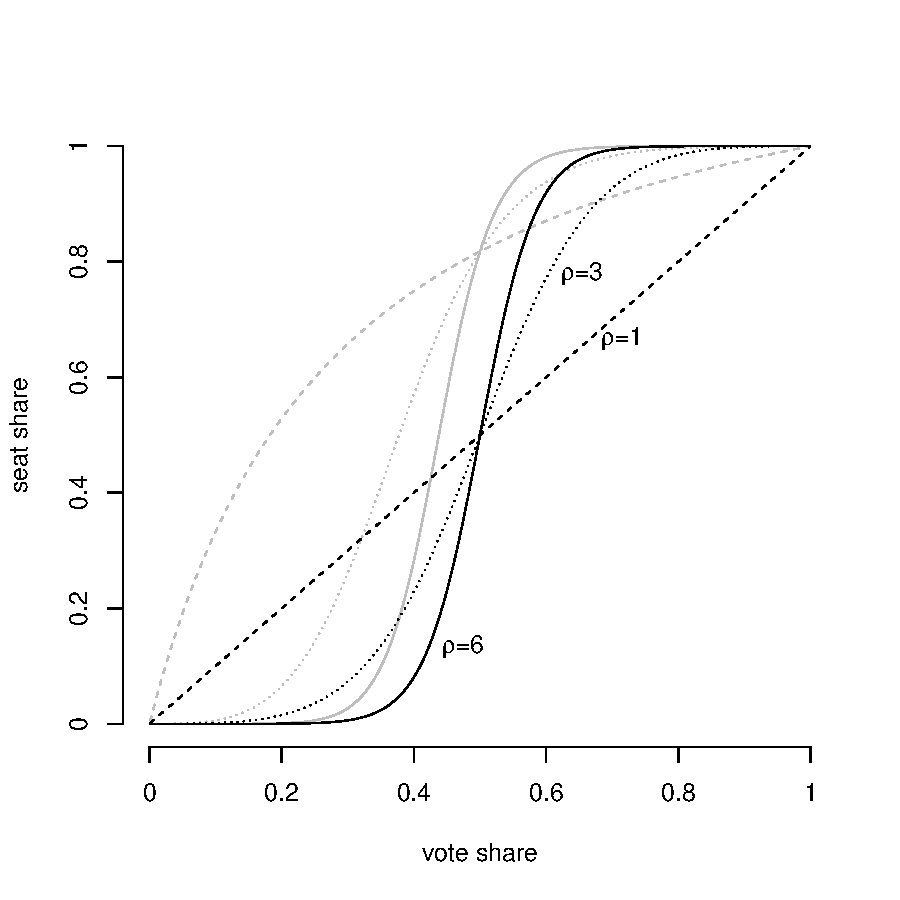
\includegraphics[width=.55\columnwidth]{rhoExample.pdf} 
    %% Created by tikzDevice version 0.8.1 on 2015-07-09 20:36:17
% !TEX encoding = UTF-8 Unicode
\begin{tikzpicture}[x=1pt,y=1pt]
\definecolor{fillColor}{RGB}{255,255,255}
\path[use as bounding box,fill=fillColor,fill opacity=0.00] (0,0) rectangle (289.08,289.08);
\begin{scope}
\path[clip] (  0.00,  0.00) rectangle (289.08,289.08);
\definecolor{drawColor}{RGB}{0,0,0}

\node[text=drawColor,anchor=base,inner sep=0pt, outer sep=0pt, scale=  1.00] at (156.54, 15.60) {vote share};

\node[text=drawColor,rotate= 90.00,anchor=base,inner sep=0pt, outer sep=0pt, scale=  1.00] at ( 10.80,150.54) {seat share};
\end{scope}
\begin{scope}
\path[clip] (  0.00,  0.00) rectangle (289.08,289.08);
\definecolor{drawColor}{RGB}{0,0,0}

\path[draw=drawColor,line width= 0.4pt,line join=round,line cap=round] ( 57.15, 61.20) -- (255.93, 61.20);

\path[draw=drawColor,line width= 0.4pt,line join=round,line cap=round] ( 57.15, 61.20) -- ( 57.15, 55.20);

\path[draw=drawColor,line width= 0.4pt,line join=round,line cap=round] ( 96.91, 61.20) -- ( 96.91, 55.20);

\path[draw=drawColor,line width= 0.4pt,line join=round,line cap=round] (136.66, 61.20) -- (136.66, 55.20);

\path[draw=drawColor,line width= 0.4pt,line join=round,line cap=round] (176.42, 61.20) -- (176.42, 55.20);

\path[draw=drawColor,line width= 0.4pt,line join=round,line cap=round] (216.17, 61.20) -- (216.17, 55.20);

\path[draw=drawColor,line width= 0.4pt,line join=round,line cap=round] (255.93, 61.20) -- (255.93, 55.20);

\node[text=drawColor,anchor=base,inner sep=0pt, outer sep=0pt, scale=  1.00] at ( 57.15, 39.60) {0};

\node[text=drawColor,anchor=base,inner sep=0pt, outer sep=0pt, scale=  1.00] at ( 96.91, 39.60) {0.2};

\node[text=drawColor,anchor=base,inner sep=0pt, outer sep=0pt, scale=  1.00] at (136.66, 39.60) {0.4};

\node[text=drawColor,anchor=base,inner sep=0pt, outer sep=0pt, scale=  1.00] at (176.42, 39.60) {0.6};

\node[text=drawColor,anchor=base,inner sep=0pt, outer sep=0pt, scale=  1.00] at (216.17, 39.60) {0.8};

\node[text=drawColor,anchor=base,inner sep=0pt, outer sep=0pt, scale=  1.00] at (255.93, 39.60) {1};

\path[draw=drawColor,line width= 0.4pt,line join=round,line cap=round] ( 49.20, 67.82) -- ( 49.20,233.26);

\path[draw=drawColor,line width= 0.4pt,line join=round,line cap=round] ( 49.20, 67.82) -- ( 43.20, 67.82);

\path[draw=drawColor,line width= 0.4pt,line join=round,line cap=round] ( 49.20,100.91) -- ( 43.20,100.91);

\path[draw=drawColor,line width= 0.4pt,line join=round,line cap=round] ( 49.20,134.00) -- ( 43.20,134.00);

\path[draw=drawColor,line width= 0.4pt,line join=round,line cap=round] ( 49.20,167.08) -- ( 43.20,167.08);

\path[draw=drawColor,line width= 0.4pt,line join=round,line cap=round] ( 49.20,200.17) -- ( 43.20,200.17);

\path[draw=drawColor,line width= 0.4pt,line join=round,line cap=round] ( 49.20,233.26) -- ( 43.20,233.26);

\node[text=drawColor,rotate= 90.00,anchor=base,inner sep=0pt, outer sep=0pt, scale=  1.00] at ( 34.80, 67.82) {0};

\node[text=drawColor,rotate= 90.00,anchor=base,inner sep=0pt, outer sep=0pt, scale=  1.00] at ( 34.80,100.91) {0.2};

\node[text=drawColor,rotate= 90.00,anchor=base,inner sep=0pt, outer sep=0pt, scale=  1.00] at ( 34.80,134.00) {0.4};

\node[text=drawColor,rotate= 90.00,anchor=base,inner sep=0pt, outer sep=0pt, scale=  1.00] at ( 34.80,167.08) {0.6};

\node[text=drawColor,rotate= 90.00,anchor=base,inner sep=0pt, outer sep=0pt, scale=  1.00] at ( 34.80,200.17) {0.8};

\node[text=drawColor,rotate= 90.00,anchor=base,inner sep=0pt, outer sep=0pt, scale=  1.00] at ( 34.80,233.26) {1};
\end{scope}
\begin{scope}
\path[clip] ( 49.20, 61.20) rectangle (263.88,239.88);
\definecolor{drawColor}{RGB}{190,190,190}

\path[draw=drawColor,line width= 0.4pt,dash pattern=on 4pt off 4pt ,line join=round,line cap=round] ( 57.35, 68.56) --
	( 57.55, 69.29) --
	( 57.75, 70.02) --
	( 57.95, 70.74) --
	( 58.14, 71.46) --
	( 58.34, 72.18) --
	( 58.54, 72.88) --
	( 58.74, 73.59) --
	( 58.94, 74.29) --
	( 59.14, 74.98) --
	( 59.34, 75.67) --
	( 59.54, 76.36) --
	( 59.74, 77.04) --
	( 59.93, 77.72) --
	( 60.13, 78.39) --
	( 60.33, 79.06) --
	( 60.53, 79.72) --
	( 60.73, 80.38) --
	( 60.93, 81.03) --
	( 61.13, 81.68) --
	( 61.33, 82.33) --
	( 61.52, 82.97) --
	( 61.72, 83.61) --
	( 61.92, 84.24) --
	( 62.12, 84.87) --
	( 62.32, 85.50) --
	( 62.52, 86.12) --
	( 62.72, 86.73) --
	( 62.92, 87.35) --
	( 63.11, 87.96) --
	( 63.31, 88.56) --
	( 63.51, 89.17) --
	( 63.71, 89.76) --
	( 63.91, 90.36) --
	( 64.11, 90.95) --
	( 64.31, 91.54) --
	( 64.51, 92.12) --
	( 64.70, 92.70) --
	( 64.90, 93.28) --
	( 65.10, 93.85) --
	( 65.30, 94.42) --
	( 65.50, 94.99) --
	( 65.70, 95.55) --
	( 65.90, 96.11) --
	( 66.10, 96.66) --
	( 66.29, 97.22) --
	( 66.49, 97.77) --
	( 66.69, 98.31) --
	( 66.89, 98.85) --
	( 67.09, 99.39) --
	( 67.29, 99.93) --
	( 67.49,100.46) --
	( 67.69,100.99) --
	( 67.89,101.52) --
	( 68.08,102.04) --
	( 68.28,102.57) --
	( 68.48,103.08) --
	( 68.68,103.60) --
	( 68.88,104.11) --
	( 69.08,104.62) --
	( 69.28,105.12) --
	( 69.48,105.63) --
	( 69.67,106.13) --
	( 69.87,106.62) --
	( 70.07,107.12) --
	( 70.27,107.61) --
	( 70.47,108.10) --
	( 70.67,108.59) --
	( 70.87,109.07) --
	( 71.07,109.55) --
	( 71.26,110.03) --
	( 71.46,110.50) --
	( 71.66,110.98) --
	( 71.86,111.45) --
	( 72.06,111.91) --
	( 72.26,112.38) --
	( 72.46,112.84) --
	( 72.66,113.30) --
	( 72.85,113.76) --
	( 73.05,114.21) --
	( 73.25,114.67) --
	( 73.45,115.12) --
	( 73.65,115.56) --
	( 73.85,116.01) --
	( 74.05,116.45) --
	( 74.25,116.89) --
	( 74.44,117.33) --
	( 74.64,117.76) --
	( 74.84,118.20) --
	( 75.04,118.63) --
	( 75.24,119.06) --
	( 75.44,119.48) --
	( 75.64,119.91) --
	( 75.84,120.33) --
	( 76.03,120.75) --
	( 76.23,121.17) --
	( 76.43,121.58) --
	( 76.63,122.00) --
	( 76.83,122.41) --
	( 77.03,122.82) --
	( 77.23,123.22) --
	( 77.43,123.63) --
	( 77.63,124.03) --
	( 77.82,124.43) --
	( 78.02,124.83) --
	( 78.22,125.23) --
	( 78.42,125.62) --
	( 78.62,126.01) --
	( 78.82,126.40) --
	( 79.02,126.79) --
	( 79.22,127.18) --
	( 79.41,127.56) --
	( 79.61,127.95) --
	( 79.81,128.33) --
	( 80.01,128.71) --
	( 80.21,129.08) --
	( 80.41,129.46) --
	( 80.61,129.83) --
	( 80.81,130.20) --
	( 81.00,130.57) --
	( 81.20,130.94) --
	( 81.40,131.31) --
	( 81.60,131.67) --
	( 81.80,132.04) --
	( 82.00,132.40) --
	( 82.20,132.76) --
	( 82.40,133.11) --
	( 82.59,133.47) --
	( 82.79,133.82) --
	( 82.99,134.17) --
	( 83.19,134.53) --
	( 83.39,134.87) --
	( 83.59,135.22) --
	( 83.79,135.57) --
	( 83.99,135.91) --
	( 84.18,136.25) --
	( 84.38,136.59) --
	( 84.58,136.93) --
	( 84.78,137.27) --
	( 84.98,137.61) --
	( 85.18,137.94) --
	( 85.38,138.27) --
	( 85.58,138.60) --
	( 85.78,138.93) --
	( 85.97,139.26) --
	( 86.17,139.59) --
	( 86.37,139.91) --
	( 86.57,140.24) --
	( 86.77,140.56) --
	( 86.97,140.88) --
	( 87.17,141.20) --
	( 87.37,141.52) --
	( 87.56,141.83) --
	( 87.76,142.15) --
	( 87.96,142.46) --
	( 88.16,142.77) --
	( 88.36,143.09) --
	( 88.56,143.39) --
	( 88.76,143.70) --
	( 88.96,144.01) --
	( 89.15,144.31) --
	( 89.35,144.62) --
	( 89.55,144.92) --
	( 89.75,145.22) --
	( 89.95,145.52) --
	( 90.15,145.82) --
	( 90.35,146.12) --
	( 90.55,146.41) --
	( 90.74,146.71) --
	( 90.94,147.00) --
	( 91.14,147.29) --
	( 91.34,147.58) --
	( 91.54,147.87) --
	( 91.74,148.16) --
	( 91.94,148.45) --
	( 92.14,148.73) --
	( 92.33,149.02) --
	( 92.53,149.30) --
	( 92.73,149.58) --
	( 92.93,149.86) --
	( 93.13,150.14) --
	( 93.33,150.42) --
	( 93.53,150.70) --
	( 93.73,150.98) --
	( 93.92,151.25) --
	( 94.12,151.52) --
	( 94.32,151.80) --
	( 94.52,152.07) --
	( 94.72,152.34) --
	( 94.92,152.61) --
	( 95.12,152.88) --
	( 95.32,153.14) --
	( 95.52,153.41) --
	( 95.71,153.67) --
	( 95.91,153.94) --
	( 96.11,154.20) --
	( 96.31,154.46) --
	( 96.51,154.72) --
	( 96.71,154.98) --
	( 96.91,155.24) --
	( 97.11,155.50) --
	( 97.30,155.75) --
	( 97.50,156.01) --
	( 97.70,156.26) --
	( 97.90,156.51) --
	( 98.10,156.77) --
	( 98.30,157.02) --
	( 98.50,157.27) --
	( 98.70,157.51) --
	( 98.89,157.76) --
	( 99.09,158.01) --
	( 99.29,158.26) --
	( 99.49,158.50) --
	( 99.69,158.74) --
	( 99.89,158.99) --
	(100.09,159.23) --
	(100.29,159.47) --
	(100.48,159.71) --
	(100.68,159.95) --
	(100.88,160.19) --
	(101.08,160.43) --
	(101.28,160.66) --
	(101.48,160.90) --
	(101.68,161.13) --
	(101.88,161.37) --
	(102.07,161.60) --
	(102.27,161.83) --
	(102.47,162.06) --
	(102.67,162.29) --
	(102.87,162.52) --
	(103.07,162.75) --
	(103.27,162.98) --
	(103.47,163.20) --
	(103.67,163.43) --
	(103.86,163.65) --
	(104.06,163.88) --
	(104.26,164.10) --
	(104.46,164.32) --
	(104.66,164.54) --
	(104.86,164.76) --
	(105.06,164.98) --
	(105.26,165.20) --
	(105.45,165.42) --
	(105.65,165.64) --
	(105.85,165.85) --
	(106.05,166.07) --
	(106.25,166.28) --
	(106.45,166.50) --
	(106.65,166.71) --
	(106.85,166.92) --
	(107.04,167.13) --
	(107.24,167.34) --
	(107.44,167.55) --
	(107.64,167.76) --
	(107.84,167.97) --
	(108.04,168.18) --
	(108.24,168.39) --
	(108.44,168.59) --
	(108.63,168.80) --
	(108.83,169.00) --
	(109.03,169.21) --
	(109.23,169.41) --
	(109.43,169.61) --
	(109.63,169.81) --
	(109.83,170.02) --
	(110.03,170.22) --
	(110.22,170.41) --
	(110.42,170.61) --
	(110.62,170.81) --
	(110.82,171.01) --
	(111.02,171.21) --
	(111.22,171.40) --
	(111.42,171.60) --
	(111.62,171.79) --
	(111.81,171.99) --
	(112.01,172.18) --
	(112.21,172.37) --
	(112.41,172.56) --
	(112.61,172.75) --
	(112.81,172.94) --
	(113.01,173.13) --
	(113.21,173.32) --
	(113.41,173.51) --
	(113.60,173.70) --
	(113.80,173.89) --
	(114.00,174.07) --
	(114.20,174.26) --
	(114.40,174.44) --
	(114.60,174.63) --
	(114.80,174.81) --
	(115.00,175.00) --
	(115.19,175.18) --
	(115.39,175.36) --
	(115.59,175.54) --
	(115.79,175.72) --
	(115.99,175.90) --
	(116.19,176.08) --
	(116.39,176.26) --
	(116.59,176.44) --
	(116.78,176.62) --
	(116.98,176.79) --
	(117.18,176.97) --
	(117.38,177.15) --
	(117.58,177.32) --
	(117.78,177.50) --
	(117.98,177.67) --
	(118.18,177.84) --
	(118.37,178.02) --
	(118.57,178.19) --
	(118.77,178.36) --
	(118.97,178.53) --
	(119.17,178.70) --
	(119.37,178.87) --
	(119.57,179.04) --
	(119.77,179.21) --
	(119.96,179.38) --
	(120.16,179.55) --
	(120.36,179.72) --
	(120.56,179.88) --
	(120.76,180.05) --
	(120.96,180.21) --
	(121.16,180.38) --
	(121.36,180.54) --
	(121.56,180.71) --
	(121.75,180.87) --
	(121.95,181.03) --
	(122.15,181.20) --
	(122.35,181.36) --
	(122.55,181.52) --
	(122.75,181.68) --
	(122.95,181.84) --
	(123.15,182.00) --
	(123.34,182.16) --
	(123.54,182.32) --
	(123.74,182.48) --
	(123.94,182.63) --
	(124.14,182.79) --
	(124.34,182.95) --
	(124.54,183.10) --
	(124.74,183.26) --
	(124.93,183.42) --
	(125.13,183.57) --
	(125.33,183.72) --
	(125.53,183.88) --
	(125.73,184.03) --
	(125.93,184.18) --
	(126.13,184.34) --
	(126.33,184.49) --
	(126.52,184.64) --
	(126.72,184.79) --
	(126.92,184.94) --
	(127.12,185.09) --
	(127.32,185.24) --
	(127.52,185.39) --
	(127.72,185.54) --
	(127.92,185.69) --
	(128.11,185.83) --
	(128.31,185.98) --
	(128.51,186.13) --
	(128.71,186.27) --
	(128.91,186.42) --
	(129.11,186.56) --
	(129.31,186.71) --
	(129.51,186.85) --
	(129.70,187.00) --
	(129.90,187.14) --
	(130.10,187.28) --
	(130.30,187.43) --
	(130.50,187.57) --
	(130.70,187.71) --
	(130.90,187.85) --
	(131.10,187.99) --
	(131.30,188.13) --
	(131.49,188.27) --
	(131.69,188.41) --
	(131.89,188.55) --
	(132.09,188.69) --
	(132.29,188.83) --
	(132.49,188.97) --
	(132.69,189.11) --
	(132.89,189.24) --
	(133.08,189.38) --
	(133.28,189.52) --
	(133.48,189.65) --
	(133.68,189.79) --
	(133.88,189.92) --
	(134.08,190.06) --
	(134.28,190.19) --
	(134.48,190.33) --
	(134.67,190.46) --
	(134.87,190.59) --
	(135.07,190.73) --
	(135.27,190.86) --
	(135.47,190.99) --
	(135.67,191.12) --
	(135.87,191.25) --
	(136.07,191.38) --
	(136.26,191.51) --
	(136.46,191.64) --
	(136.66,191.77) --
	(136.86,191.90) --
	(137.06,192.03) --
	(137.26,192.16) --
	(137.46,192.29) --
	(137.66,192.42) --
	(137.85,192.54) --
	(138.05,192.67) --
	(138.25,192.80) --
	(138.45,192.93) --
	(138.65,193.05) --
	(138.85,193.18) --
	(139.05,193.30) --
	(139.25,193.43) --
	(139.45,193.55) --
	(139.64,193.68) --
	(139.84,193.80) --
	(140.04,193.92) --
	(140.24,194.05) --
	(140.44,194.17) --
	(140.64,194.29) --
	(140.84,194.41) --
	(141.04,194.54) --
	(141.23,194.66) --
	(141.43,194.78) --
	(141.63,194.90) --
	(141.83,195.02) --
	(142.03,195.14) --
	(142.23,195.26) --
	(142.43,195.38) --
	(142.63,195.50) --
	(142.82,195.62) --
	(143.02,195.73) --
	(143.22,195.85) --
	(143.42,195.97) --
	(143.62,196.09) --
	(143.82,196.21) --
	(144.02,196.32) --
	(144.22,196.44) --
	(144.41,196.55) --
	(144.61,196.67) --
	(144.81,196.79) --
	(145.01,196.90) --
	(145.21,197.02) --
	(145.41,197.13) --
	(145.61,197.24) --
	(145.81,197.36) --
	(146.00,197.47) --
	(146.20,197.59) --
	(146.40,197.70) --
	(146.60,197.81) --
	(146.80,197.92) --
	(147.00,198.04) --
	(147.20,198.15) --
	(147.40,198.26) --
	(147.59,198.37) --
	(147.79,198.48) --
	(147.99,198.59) --
	(148.19,198.70) --
	(148.39,198.81) --
	(148.59,198.92) --
	(148.79,199.03) --
	(148.99,199.14) --
	(149.19,199.25) --
	(149.38,199.36) --
	(149.58,199.47) --
	(149.78,199.57) --
	(149.98,199.68) --
	(150.18,199.79) --
	(150.38,199.90) --
	(150.58,200.00) --
	(150.78,200.11) --
	(150.97,200.22) --
	(151.17,200.32) --
	(151.37,200.43) --
	(151.57,200.53) --
	(151.77,200.64) --
	(151.97,200.74) --
	(152.17,200.85) --
	(152.37,200.95) --
	(152.56,201.06) --
	(152.76,201.16) --
	(152.96,201.26) --
	(153.16,201.37) --
	(153.36,201.47) --
	(153.56,201.57) --
	(153.76,201.67) --
	(153.96,201.78) --
	(154.15,201.88) --
	(154.35,201.98) --
	(154.55,202.08) --
	(154.75,202.18) --
	(154.95,202.28) --
	(155.15,202.38) --
	(155.35,202.48) --
	(155.55,202.58) --
	(155.74,202.68) --
	(155.94,202.78) --
	(156.14,202.88) --
	(156.34,202.98) --
	(156.54,203.08) --
	(156.74,203.18) --
	(156.94,203.28) --
	(157.14,203.38) --
	(157.34,203.47) --
	(157.53,203.57) --
	(157.73,203.67) --
	(157.93,203.77) --
	(158.13,203.86) --
	(158.33,203.96) --
	(158.53,204.06) --
	(158.73,204.15) --
	(158.93,204.25) --
	(159.12,204.34) --
	(159.32,204.44) --
	(159.52,204.53) --
	(159.72,204.63) --
	(159.92,204.72) --
	(160.12,204.82) --
	(160.32,204.91) --
	(160.52,205.01) --
	(160.71,205.10) --
	(160.91,205.19) --
	(161.11,205.29) --
	(161.31,205.38) --
	(161.51,205.47) --
	(161.71,205.57) --
	(161.91,205.66) --
	(162.11,205.75) --
	(162.30,205.84) --
	(162.50,205.93) --
	(162.70,206.02) --
	(162.90,206.12) --
	(163.10,206.21) --
	(163.30,206.30) --
	(163.50,206.39) --
	(163.70,206.48) --
	(163.89,206.57) --
	(164.09,206.66) --
	(164.29,206.75) --
	(164.49,206.84) --
	(164.69,206.93) --
	(164.89,207.02) --
	(165.09,207.11) --
	(165.29,207.19) --
	(165.48,207.28) --
	(165.68,207.37) --
	(165.88,207.46) --
	(166.08,207.55) --
	(166.28,207.63) --
	(166.48,207.72) --
	(166.68,207.81) --
	(166.88,207.90) --
	(167.08,207.98) --
	(167.27,208.07) --
	(167.47,208.16) --
	(167.67,208.24) --
	(167.87,208.33) --
	(168.07,208.41) --
	(168.27,208.50) --
	(168.47,208.58) --
	(168.67,208.67) --
	(168.86,208.75) --
	(169.06,208.84) --
	(169.26,208.92) --
	(169.46,209.01) --
	(169.66,209.09) --
	(169.86,209.18) --
	(170.06,209.26) --
	(170.26,209.34) --
	(170.45,209.43) --
	(170.65,209.51) --
	(170.85,209.59) --
	(171.05,209.67) --
	(171.25,209.76) --
	(171.45,209.84) --
	(171.65,209.92) --
	(171.85,210.00) --
	(172.04,210.09) --
	(172.24,210.17) --
	(172.44,210.25) --
	(172.64,210.33) --
	(172.84,210.41) --
	(173.04,210.49) --
	(173.24,210.57) --
	(173.44,210.65) --
	(173.63,210.73) --
	(173.83,210.81) --
	(174.03,210.89) --
	(174.23,210.97) --
	(174.43,211.05) --
	(174.63,211.13) --
	(174.83,211.21) --
	(175.03,211.29) --
	(175.23,211.37) --
	(175.42,211.45) --
	(175.62,211.53) --
	(175.82,211.60) --
	(176.02,211.68) --
	(176.22,211.76) --
	(176.42,211.84) --
	(176.62,211.92) --
	(176.82,211.99) --
	(177.01,212.07) --
	(177.21,212.15) --
	(177.41,212.22) --
	(177.61,212.30) --
	(177.81,212.38) --
	(178.01,212.45) --
	(178.21,212.53) --
	(178.41,212.61) --
	(178.60,212.68) --
	(178.80,212.76) --
	(179.00,212.83) --
	(179.20,212.91) --
	(179.40,212.98) --
	(179.60,213.06) --
	(179.80,213.13) --
	(180.00,213.21) --
	(180.19,213.28) --
	(180.39,213.36) --
	(180.59,213.43) --
	(180.79,213.51) --
	(180.99,213.58) --
	(181.19,213.65) --
	(181.39,213.73) --
	(181.59,213.80) --
	(181.78,213.87) --
	(181.98,213.95) --
	(182.18,214.02) --
	(182.38,214.09) --
	(182.58,214.17) --
	(182.78,214.24) --
	(182.98,214.31) --
	(183.18,214.38) --
	(183.38,214.46) --
	(183.57,214.53) --
	(183.77,214.60) --
	(183.97,214.67) --
	(184.17,214.74) --
	(184.37,214.81) --
	(184.57,214.88) --
	(184.77,214.95) --
	(184.97,215.03) --
	(185.16,215.10) --
	(185.36,215.17) --
	(185.56,215.24) --
	(185.76,215.31) --
	(185.96,215.38) --
	(186.16,215.45) --
	(186.36,215.52) --
	(186.56,215.59) --
	(186.75,215.66) --
	(186.95,215.72) --
	(187.15,215.79) --
	(187.35,215.86) --
	(187.55,215.93) --
	(187.75,216.00) --
	(187.95,216.07) --
	(188.15,216.14) --
	(188.34,216.21) --
	(188.54,216.27) --
	(188.74,216.34) --
	(188.94,216.41) --
	(189.14,216.48) --
	(189.34,216.54) --
	(189.54,216.61) --
	(189.74,216.68) --
	(189.93,216.75) --
	(190.13,216.81) --
	(190.33,216.88) --
	(190.53,216.95) --
	(190.73,217.01) --
	(190.93,217.08) --
	(191.13,217.15) --
	(191.33,217.21) --
	(191.52,217.28) --
	(191.72,217.34) --
	(191.92,217.41) --
	(192.12,217.48) --
	(192.32,217.54) --
	(192.52,217.61) --
	(192.72,217.67) --
	(192.92,217.74) --
	(193.12,217.80) --
	(193.31,217.87) --
	(193.51,217.93) --
	(193.71,218.00) --
	(193.91,218.06) --
	(194.11,218.12) --
	(194.31,218.19) --
	(194.51,218.25) --
	(194.71,218.32) --
	(194.90,218.38) --
	(195.10,218.44) --
	(195.30,218.51) --
	(195.50,218.57) --
	(195.70,218.63) --
	(195.90,218.70) --
	(196.10,218.76) --
	(196.30,218.82) --
	(196.49,218.88) --
	(196.69,218.95) --
	(196.89,219.01) --
	(197.09,219.07) --
	(197.29,219.13) --
	(197.49,219.20) --
	(197.69,219.26) --
	(197.89,219.32) --
	(198.08,219.38) --
	(198.28,219.44) --
	(198.48,219.50) --
	(198.68,219.57) --
	(198.88,219.63) --
	(199.08,219.69) --
	(199.28,219.75) --
	(199.48,219.81) --
	(199.67,219.87) --
	(199.87,219.93) --
	(200.07,219.99) --
	(200.27,220.05) --
	(200.47,220.11) --
	(200.67,220.17) --
	(200.87,220.23) --
	(201.07,220.29) --
	(201.26,220.35) --
	(201.46,220.41) --
	(201.66,220.47) --
	(201.86,220.53) --
	(202.06,220.59) --
	(202.26,220.65) --
	(202.46,220.71) --
	(202.66,220.77) --
	(202.86,220.83) --
	(203.05,220.88) --
	(203.25,220.94) --
	(203.45,221.00) --
	(203.65,221.06) --
	(203.85,221.12) --
	(204.05,221.18) --
	(204.25,221.23) --
	(204.45,221.29) --
	(204.64,221.35) --
	(204.84,221.41) --
	(205.04,221.47) --
	(205.24,221.52) --
	(205.44,221.58) --
	(205.64,221.64) --
	(205.84,221.69) --
	(206.04,221.75) --
	(206.23,221.81) --
	(206.43,221.87) --
	(206.63,221.92) --
	(206.83,221.98) --
	(207.03,222.04) --
	(207.23,222.09) --
	(207.43,222.15) --
	(207.63,222.20) --
	(207.82,222.26) --
	(208.02,222.32) --
	(208.22,222.37) --
	(208.42,222.43) --
	(208.62,222.48) --
	(208.82,222.54) --
	(209.02,222.59) --
	(209.22,222.65) --
	(209.41,222.70) --
	(209.61,222.76) --
	(209.81,222.81) --
	(210.01,222.87) --
	(210.21,222.92) --
	(210.41,222.98) --
	(210.61,223.03) --
	(210.81,223.09) --
	(211.01,223.14) --
	(211.20,223.20) --
	(211.40,223.25) --
	(211.60,223.31) --
	(211.80,223.36) --
	(212.00,223.41) --
	(212.20,223.47) --
	(212.40,223.52) --
	(212.60,223.57) --
	(212.79,223.63) --
	(212.99,223.68) --
	(213.19,223.73) --
	(213.39,223.79) --
	(213.59,223.84) --
	(213.79,223.89) --
	(213.99,223.95) --
	(214.19,224.00) --
	(214.38,224.05) --
	(214.58,224.10) --
	(214.78,224.16) --
	(214.98,224.21) --
	(215.18,224.26) --
	(215.38,224.31) --
	(215.58,224.37) --
	(215.78,224.42) --
	(215.97,224.47) --
	(216.17,224.52) --
	(216.37,224.57) --
	(216.57,224.62) --
	(216.77,224.68) --
	(216.97,224.73) --
	(217.17,224.78) --
	(217.37,224.83) --
	(217.56,224.88) --
	(217.76,224.93) --
	(217.96,224.98) --
	(218.16,225.03) --
	(218.36,225.08) --
	(218.56,225.14) --
	(218.76,225.19) --
	(218.96,225.24) --
	(219.15,225.29) --
	(219.35,225.34) --
	(219.55,225.39) --
	(219.75,225.44) --
	(219.95,225.49) --
	(220.15,225.54) --
	(220.35,225.59) --
	(220.55,225.64) --
	(220.75,225.69) --
	(220.94,225.74) --
	(221.14,225.79) --
	(221.34,225.83) --
	(221.54,225.88) --
	(221.74,225.93) --
	(221.94,225.98) --
	(222.14,226.03) --
	(222.34,226.08) --
	(222.53,226.13) --
	(222.73,226.18) --
	(222.93,226.23) --
	(223.13,226.28) --
	(223.33,226.32) --
	(223.53,226.37) --
	(223.73,226.42) --
	(223.93,226.47) --
	(224.12,226.52) --
	(224.32,226.57) --
	(224.52,226.61) --
	(224.72,226.66) --
	(224.92,226.71) --
	(225.12,226.76) --
	(225.32,226.80) --
	(225.52,226.85) --
	(225.71,226.90) --
	(225.91,226.95) --
	(226.11,226.99) --
	(226.31,227.04) --
	(226.51,227.09) --
	(226.71,227.14) --
	(226.91,227.18) --
	(227.11,227.23) --
	(227.30,227.28) --
	(227.50,227.32) --
	(227.70,227.37) --
	(227.90,227.42) --
	(228.10,227.46) --
	(228.30,227.51) --
	(228.50,227.56) --
	(228.70,227.60) --
	(228.90,227.65) --
	(229.09,227.69) --
	(229.29,227.74) --
	(229.49,227.79) --
	(229.69,227.83) --
	(229.89,227.88) --
	(230.09,227.92) --
	(230.29,227.97) --
	(230.49,228.02) --
	(230.68,228.06) --
	(230.88,228.11) --
	(231.08,228.15) --
	(231.28,228.20) --
	(231.48,228.24) --
	(231.68,228.29) --
	(231.88,228.33) --
	(232.08,228.38) --
	(232.27,228.42) --
	(232.47,228.47) --
	(232.67,228.51) --
	(232.87,228.56) --
	(233.07,228.60) --
	(233.27,228.64) --
	(233.47,228.69) --
	(233.67,228.73) --
	(233.86,228.78) --
	(234.06,228.82) --
	(234.26,228.87) --
	(234.46,228.91) --
	(234.66,228.95) --
	(234.86,229.00) --
	(235.06,229.04) --
	(235.26,229.09) --
	(235.45,229.13) --
	(235.65,229.17) --
	(235.85,229.22) --
	(236.05,229.26) --
	(236.25,229.30) --
	(236.45,229.35) --
	(236.65,229.39) --
	(236.85,229.43) --
	(237.04,229.48) --
	(237.24,229.52) --
	(237.44,229.56) --
	(237.64,229.60) --
	(237.84,229.65) --
	(238.04,229.69) --
	(238.24,229.73) --
	(238.44,229.78) --
	(238.64,229.82) --
	(238.83,229.86) --
	(239.03,229.90) --
	(239.23,229.94) --
	(239.43,229.99) --
	(239.63,230.03) --
	(239.83,230.07) --
	(240.03,230.11) --
	(240.23,230.16) --
	(240.42,230.20) --
	(240.62,230.24) --
	(240.82,230.28) --
	(241.02,230.32) --
	(241.22,230.36) --
	(241.42,230.41) --
	(241.62,230.45) --
	(241.82,230.49) --
	(242.01,230.53) --
	(242.21,230.57) --
	(242.41,230.61) --
	(242.61,230.65) --
	(242.81,230.69) --
	(243.01,230.74) --
	(243.21,230.78) --
	(243.41,230.82) --
	(243.60,230.86) --
	(243.80,230.90) --
	(244.00,230.94) --
	(244.20,230.98) --
	(244.40,231.02) --
	(244.60,231.06) --
	(244.80,231.10) --
	(245.00,231.14) --
	(245.19,231.18) --
	(245.39,231.22) --
	(245.59,231.26) --
	(245.79,231.30) --
	(245.99,231.34) --
	(246.19,231.38) --
	(246.39,231.42) --
	(246.59,231.46) --
	(246.79,231.50) --
	(246.98,231.54) --
	(247.18,231.58) --
	(247.38,231.62) --
	(247.58,231.66) --
	(247.78,231.70) --
	(247.98,231.74) --
	(248.18,231.78) --
	(248.38,231.82) --
	(248.57,231.86) --
	(248.77,231.90) --
	(248.97,231.93) --
	(249.17,231.97) --
	(249.37,232.01) --
	(249.57,232.05) --
	(249.77,232.09) --
	(249.97,232.13) --
	(250.16,232.17) --
	(250.36,232.21) --
	(250.56,232.24) --
	(250.76,232.28) --
	(250.96,232.32) --
	(251.16,232.36) --
	(251.36,232.40) --
	(251.56,232.44) --
	(251.75,232.47) --
	(251.95,232.51) --
	(252.15,232.55) --
	(252.35,232.59) --
	(252.55,232.63) --
	(252.75,232.66) --
	(252.95,232.70) --
	(253.15,232.74) --
	(253.34,232.78) --
	(253.54,232.82) --
	(253.74,232.85) --
	(253.94,232.89) --
	(254.14,232.93) --
	(254.34,232.97) --
	(254.54,233.00) --
	(254.74,233.04) --
	(254.93,233.08) --
	(255.13,233.11) --
	(255.33,233.15) --
	(255.53,233.19) --
	(255.73,233.23);

\path[draw=drawColor,line width= 0.4pt,dash pattern=on 1pt off 3pt ,line join=round,line cap=round] ( 57.35, 67.82) --
	( 57.55, 67.82) --
	( 57.75, 67.82) --
	( 57.95, 67.82) --
	( 58.14, 67.82) --
	( 58.34, 67.82) --
	( 58.54, 67.82) --
	( 58.74, 67.82) --
	( 58.94, 67.82) --
	( 59.14, 67.82) --
	( 59.34, 67.82) --
	( 59.54, 67.82) --
	( 59.74, 67.82) --
	( 59.93, 67.82) --
	( 60.13, 67.82) --
	( 60.33, 67.82) --
	( 60.53, 67.82) --
	( 60.73, 67.82) --
	( 60.93, 67.82) --
	( 61.13, 67.82) --
	( 61.33, 67.83) --
	( 61.52, 67.83) --
	( 61.72, 67.83) --
	( 61.92, 67.83) --
	( 62.12, 67.83) --
	( 62.32, 67.83) --
	( 62.52, 67.83) --
	( 62.72, 67.84) --
	( 62.92, 67.84) --
	( 63.11, 67.84) --
	( 63.31, 67.84) --
	( 63.51, 67.84) --
	( 63.71, 67.85) --
	( 63.91, 67.85) --
	( 64.11, 67.85) --
	( 64.31, 67.86) --
	( 64.51, 67.86) --
	( 64.70, 67.86) --
	( 64.90, 67.87) --
	( 65.10, 67.87) --
	( 65.30, 67.88) --
	( 65.50, 67.88) --
	( 65.70, 67.89) --
	( 65.90, 67.89) --
	( 66.10, 67.90) --
	( 66.29, 67.90) --
	( 66.49, 67.91) --
	( 66.69, 67.91) --
	( 66.89, 67.92) --
	( 67.09, 67.93) --
	( 67.29, 67.93) --
	( 67.49, 67.94) --
	( 67.69, 67.95) --
	( 67.89, 67.96) --
	( 68.08, 67.96) --
	( 68.28, 67.97) --
	( 68.48, 67.98) --
	( 68.68, 67.99) --
	( 68.88, 68.00) --
	( 69.08, 68.01) --
	( 69.28, 68.02) --
	( 69.48, 68.03) --
	( 69.67, 68.04) --
	( 69.87, 68.05) --
	( 70.07, 68.07) --
	( 70.27, 68.08) --
	( 70.47, 68.09) --
	( 70.67, 68.11) --
	( 70.87, 68.12) --
	( 71.07, 68.13) --
	( 71.26, 68.15) --
	( 71.46, 68.16) --
	( 71.66, 68.18) --
	( 71.86, 68.20) --
	( 72.06, 68.21) --
	( 72.26, 68.23) --
	( 72.46, 68.25) --
	( 72.66, 68.27) --
	( 72.85, 68.28) --
	( 73.05, 68.30) --
	( 73.25, 68.32) --
	( 73.45, 68.34) --
	( 73.65, 68.37) --
	( 73.85, 68.39) --
	( 74.05, 68.41) --
	( 74.25, 68.43) --
	( 74.44, 68.46) --
	( 74.64, 68.48) --
	( 74.84, 68.51) --
	( 75.04, 68.53) --
	( 75.24, 68.56) --
	( 75.44, 68.59) --
	( 75.64, 68.61) --
	( 75.84, 68.64) --
	( 76.03, 68.67) --
	( 76.23, 68.70) --
	( 76.43, 68.73) --
	( 76.63, 68.76) --
	( 76.83, 68.80) --
	( 77.03, 68.83) --
	( 77.23, 68.86) --
	( 77.43, 68.90) --
	( 77.63, 68.93) --
	( 77.82, 68.97) --
	( 78.02, 69.01) --
	( 78.22, 69.04) --
	( 78.42, 69.08) --
	( 78.62, 69.12) --
	( 78.82, 69.16) --
	( 79.02, 69.21) --
	( 79.22, 69.25) --
	( 79.41, 69.29) --
	( 79.61, 69.34) --
	( 79.81, 69.38) --
	( 80.01, 69.43) --
	( 80.21, 69.48) --
	( 80.41, 69.52) --
	( 80.61, 69.57) --
	( 80.81, 69.63) --
	( 81.00, 69.68) --
	( 81.20, 69.73) --
	( 81.40, 69.78) --
	( 81.60, 69.84) --
	( 81.80, 69.89) --
	( 82.00, 69.95) --
	( 82.20, 70.01) --
	( 82.40, 70.07) --
	( 82.59, 70.13) --
	( 82.79, 70.19) --
	( 82.99, 70.26) --
	( 83.19, 70.32) --
	( 83.39, 70.39) --
	( 83.59, 70.45) --
	( 83.79, 70.52) --
	( 83.99, 70.59) --
	( 84.18, 70.66) --
	( 84.38, 70.73) --
	( 84.58, 70.81) --
	( 84.78, 70.88) --
	( 84.98, 70.96) --
	( 85.18, 71.03) --
	( 85.38, 71.11) --
	( 85.58, 71.19) --
	( 85.78, 71.27) --
	( 85.97, 71.36) --
	( 86.17, 71.44) --
	( 86.37, 71.53) --
	( 86.57, 71.62) --
	( 86.77, 71.70) --
	( 86.97, 71.79) --
	( 87.17, 71.89) --
	( 87.37, 71.98) --
	( 87.56, 72.08) --
	( 87.76, 72.17) --
	( 87.96, 72.27) --
	( 88.16, 72.37) --
	( 88.36, 72.47) --
	( 88.56, 72.58) --
	( 88.76, 72.68) --
	( 88.96, 72.79) --
	( 89.15, 72.90) --
	( 89.35, 73.01) --
	( 89.55, 73.12) --
	( 89.75, 73.23) --
	( 89.95, 73.35) --
	( 90.15, 73.47) --
	( 90.35, 73.58) --
	( 90.55, 73.71) --
	( 90.74, 73.83) --
	( 90.94, 73.95) --
	( 91.14, 74.08) --
	( 91.34, 74.21) --
	( 91.54, 74.34) --
	( 91.74, 74.47) --
	( 91.94, 74.60) --
	( 92.14, 74.74) --
	( 92.33, 74.88) --
	( 92.53, 75.02) --
	( 92.73, 75.16) --
	( 92.93, 75.31) --
	( 93.13, 75.45) --
	( 93.33, 75.60) --
	( 93.53, 75.75) --
	( 93.73, 75.90) --
	( 93.92, 76.06) --
	( 94.12, 76.22) --
	( 94.32, 76.37) --
	( 94.52, 76.54) --
	( 94.72, 76.70) --
	( 94.92, 76.86) --
	( 95.12, 77.03) --
	( 95.32, 77.20) --
	( 95.52, 77.37) --
	( 95.71, 77.55) --
	( 95.91, 77.73) --
	( 96.11, 77.91) --
	( 96.31, 78.09) --
	( 96.51, 78.27) --
	( 96.71, 78.46) --
	( 96.91, 78.65) --
	( 97.11, 78.84) --
	( 97.30, 79.03) --
	( 97.50, 79.23) --
	( 97.70, 79.42) --
	( 97.90, 79.62) --
	( 98.10, 79.83) --
	( 98.30, 80.03) --
	( 98.50, 80.24) --
	( 98.70, 80.45) --
	( 98.89, 80.66) --
	( 99.09, 80.88) --
	( 99.29, 81.10) --
	( 99.49, 81.32) --
	( 99.69, 81.54) --
	( 99.89, 81.77) --
	(100.09, 82.00) --
	(100.29, 82.23) --
	(100.48, 82.46) --
	(100.68, 82.70) --
	(100.88, 82.93) --
	(101.08, 83.18) --
	(101.28, 83.42) --
	(101.48, 83.67) --
	(101.68, 83.92) --
	(101.88, 84.17) --
	(102.07, 84.42) --
	(102.27, 84.68) --
	(102.47, 84.94) --
	(102.67, 85.20) --
	(102.87, 85.47) --
	(103.07, 85.74) --
	(103.27, 86.01) --
	(103.47, 86.28) --
	(103.67, 86.56) --
	(103.86, 86.84) --
	(104.06, 87.12) --
	(104.26, 87.41) --
	(104.46, 87.70) --
	(104.66, 87.99) --
	(104.86, 88.28) --
	(105.06, 88.58) --
	(105.26, 88.88) --
	(105.45, 89.18) --
	(105.65, 89.48) --
	(105.85, 89.79) --
	(106.05, 90.10) --
	(106.25, 90.41) --
	(106.45, 90.73) --
	(106.65, 91.05) --
	(106.85, 91.37) --
	(107.04, 91.69) --
	(107.24, 92.02) --
	(107.44, 92.35) --
	(107.64, 92.69) --
	(107.84, 93.02) --
	(108.04, 93.36) --
	(108.24, 93.70) --
	(108.44, 94.05) --
	(108.63, 94.39) --
	(108.83, 94.74) --
	(109.03, 95.10) --
	(109.23, 95.45) --
	(109.43, 95.81) --
	(109.63, 96.17) --
	(109.83, 96.54) --
	(110.03, 96.90) --
	(110.22, 97.27) --
	(110.42, 97.65) --
	(110.62, 98.02) --
	(110.82, 98.40) --
	(111.02, 98.78) --
	(111.22, 99.16) --
	(111.42, 99.55) --
	(111.62, 99.94) --
	(111.81,100.33) --
	(112.01,100.72) --
	(112.21,101.12) --
	(112.41,101.52) --
	(112.61,101.92) --
	(112.81,102.33) --
	(113.01,102.74) --
	(113.21,103.15) --
	(113.41,103.56) --
	(113.60,103.98) --
	(113.80,104.39) --
	(114.00,104.82) --
	(114.20,105.24) --
	(114.40,105.66) --
	(114.60,106.09) --
	(114.80,106.52) --
	(115.00,106.96) --
	(115.19,107.39) --
	(115.39,107.83) --
	(115.59,108.27) --
	(115.79,108.71) --
	(115.99,109.16) --
	(116.19,109.61) --
	(116.39,110.06) --
	(116.59,110.51) --
	(116.78,110.96) --
	(116.98,111.42) --
	(117.18,111.88) --
	(117.38,112.34) --
	(117.58,112.80) --
	(117.78,113.27) --
	(117.98,113.74) --
	(118.18,114.21) --
	(118.37,114.68) --
	(118.57,115.15) --
	(118.77,115.63) --
	(118.97,116.11) --
	(119.17,116.58) --
	(119.37,117.07) --
	(119.57,117.55) --
	(119.77,118.04) --
	(119.96,118.52) --
	(120.16,119.01) --
	(120.36,119.50) --
	(120.56,119.99) --
	(120.76,120.49) --
	(120.96,120.98) --
	(121.16,121.48) --
	(121.36,121.98) --
	(121.56,122.48) --
	(121.75,122.98) --
	(121.95,123.49) --
	(122.15,123.99) --
	(122.35,124.50) --
	(122.55,125.01) --
	(122.75,125.52) --
	(122.95,126.03) --
	(123.15,126.54) --
	(123.34,127.05) --
	(123.54,127.57) --
	(123.74,128.08) --
	(123.94,128.60) --
	(124.14,129.11) --
	(124.34,129.63) --
	(124.54,130.15) --
	(124.74,130.67) --
	(124.93,131.20) --
	(125.13,131.72) --
	(125.33,132.24) --
	(125.53,132.76) --
	(125.73,133.29) --
	(125.93,133.82) --
	(126.13,134.34) --
	(126.33,134.87) --
	(126.52,135.40) --
	(126.72,135.92) --
	(126.92,136.45) --
	(127.12,136.98) --
	(127.32,137.51) --
	(127.52,138.04) --
	(127.72,138.57) --
	(127.92,139.10) --
	(128.11,139.63) --
	(128.31,140.17) --
	(128.51,140.70) --
	(128.71,141.23) --
	(128.91,141.76) --
	(129.11,142.29) --
	(129.31,142.82) --
	(129.51,143.36) --
	(129.70,143.89) --
	(129.90,144.42) --
	(130.10,144.95) --
	(130.30,145.48) --
	(130.50,146.01) --
	(130.70,146.55) --
	(130.90,147.08) --
	(131.10,147.61) --
	(131.30,148.14) --
	(131.49,148.67) --
	(131.69,149.20) --
	(131.89,149.73) --
	(132.09,150.25) --
	(132.29,150.78) --
	(132.49,151.31) --
	(132.69,151.84) --
	(132.89,152.36) --
	(133.08,152.89) --
	(133.28,153.41) --
	(133.48,153.94) --
	(133.68,154.46) --
	(133.88,154.98) --
	(134.08,155.50) --
	(134.28,156.03) --
	(134.48,156.55) --
	(134.67,157.06) --
	(134.87,157.58) --
	(135.07,158.10) --
	(135.27,158.61) --
	(135.47,159.13) --
	(135.67,159.64) --
	(135.87,160.15) --
	(136.07,160.67) --
	(136.26,161.18) --
	(136.46,161.68) --
	(136.66,162.19) --
	(136.86,162.70) --
	(137.06,163.20) --
	(137.26,163.71) --
	(137.46,164.21) --
	(137.66,164.71) --
	(137.85,165.21) --
	(138.05,165.71) --
	(138.25,166.20) --
	(138.45,166.70) --
	(138.65,167.19) --
	(138.85,167.68) --
	(139.05,168.17) --
	(139.25,168.66) --
	(139.45,169.14) --
	(139.64,169.63) --
	(139.84,170.11) --
	(140.04,170.59) --
	(140.24,171.07) --
	(140.44,171.55) --
	(140.64,172.03) --
	(140.84,172.50) --
	(141.04,172.97) --
	(141.23,173.44) --
	(141.43,173.91) --
	(141.63,174.38) --
	(141.83,174.84) --
	(142.03,175.31) --
	(142.23,175.77) --
	(142.43,176.23) --
	(142.63,176.68) --
	(142.82,177.14) --
	(143.02,177.59) --
	(143.22,178.04) --
	(143.42,178.49) --
	(143.62,178.94) --
	(143.82,179.38) --
	(144.02,179.82) --
	(144.22,180.26) --
	(144.41,180.70) --
	(144.61,181.14) --
	(144.81,181.57) --
	(145.01,182.00) --
	(145.21,182.43) --
	(145.41,182.86) --
	(145.61,183.28) --
	(145.81,183.70) --
	(146.00,184.12) --
	(146.20,184.54) --
	(146.40,184.96) --
	(146.60,185.37) --
	(146.80,185.78) --
	(147.00,186.19) --
	(147.20,186.60) --
	(147.40,187.00) --
	(147.59,187.41) --
	(147.79,187.81) --
	(147.99,188.20) --
	(148.19,188.60) --
	(148.39,188.99) --
	(148.59,189.38) --
	(148.79,189.77) --
	(148.99,190.16) --
	(149.19,190.54) --
	(149.38,190.92) --
	(149.58,191.30) --
	(149.78,191.68) --
	(149.98,192.05) --
	(150.18,192.42) --
	(150.38,192.79) --
	(150.58,193.16) --
	(150.78,193.52) --
	(150.97,193.89) --
	(151.17,194.25) --
	(151.37,194.60) --
	(151.57,194.96) --
	(151.77,195.31) --
	(151.97,195.66) --
	(152.17,196.01) --
	(152.37,196.36) --
	(152.56,196.70) --
	(152.76,197.04) --
	(152.96,197.38) --
	(153.16,197.72) --
	(153.36,198.05) --
	(153.56,198.38) --
	(153.76,198.71) --
	(153.96,199.04) --
	(154.15,199.36) --
	(154.35,199.69) --
	(154.55,200.01) --
	(154.75,200.32) --
	(154.95,200.64) --
	(155.15,200.95) --
	(155.35,201.26) --
	(155.55,201.57) --
	(155.74,201.88) --
	(155.94,202.18) --
	(156.14,202.48) --
	(156.34,202.78) --
	(156.54,203.08) --
	(156.74,203.38) --
	(156.94,203.67) --
	(157.14,203.96) --
	(157.34,204.25) --
	(157.53,204.53) --
	(157.73,204.82) --
	(157.93,205.10) --
	(158.13,205.38) --
	(158.33,205.66) --
	(158.53,205.93) --
	(158.73,206.20) --
	(158.93,206.47) --
	(159.12,206.74) --
	(159.32,207.01) --
	(159.52,207.27) --
	(159.72,207.53) --
	(159.92,207.79) --
	(160.12,208.05) --
	(160.32,208.31) --
	(160.52,208.56) --
	(160.71,208.81) --
	(160.91,209.06) --
	(161.11,209.31) --
	(161.31,209.56) --
	(161.51,209.80) --
	(161.71,210.04) --
	(161.91,210.28) --
	(162.11,210.52) --
	(162.30,210.75) --
	(162.50,210.98) --
	(162.70,211.22) --
	(162.90,211.45) --
	(163.10,211.67) --
	(163.30,211.90) --
	(163.50,212.12) --
	(163.70,212.34) --
	(163.89,212.56) --
	(164.09,212.78) --
	(164.29,213.00) --
	(164.49,213.21) --
	(164.69,213.42) --
	(164.89,213.63) --
	(165.09,213.84) --
	(165.29,214.05) --
	(165.48,214.25) --
	(165.68,214.45) --
	(165.88,214.65) --
	(166.08,214.85) --
	(166.28,215.05) --
	(166.48,215.25) --
	(166.68,215.44) --
	(166.88,215.63) --
	(167.08,215.82) --
	(167.27,216.01) --
	(167.47,216.20) --
	(167.67,216.38) --
	(167.87,216.56) --
	(168.07,216.75) --
	(168.27,216.93) --
	(168.47,217.10) --
	(168.67,217.28) --
	(168.86,217.46) --
	(169.06,217.63) --
	(169.26,217.80) --
	(169.46,217.97) --
	(169.66,218.14) --
	(169.86,218.31) --
	(170.06,218.47) --
	(170.26,218.64) --
	(170.45,218.80) --
	(170.65,218.96) --
	(170.85,219.12) --
	(171.05,219.28) --
	(171.25,219.43) --
	(171.45,219.59) --
	(171.65,219.74) --
	(171.85,219.89) --
	(172.04,220.04) --
	(172.24,220.19) --
	(172.44,220.34) --
	(172.64,220.49) --
	(172.84,220.63) --
	(173.04,220.77) --
	(173.24,220.92) --
	(173.44,221.06) --
	(173.63,221.19) --
	(173.83,221.33) --
	(174.03,221.47) --
	(174.23,221.60) --
	(174.43,221.74) --
	(174.63,221.87) --
	(174.83,222.00) --
	(175.03,222.13) --
	(175.23,222.26) --
	(175.42,222.39) --
	(175.62,222.51) --
	(175.82,222.64) --
	(176.02,222.76) --
	(176.22,222.88) --
	(176.42,223.00) --
	(176.62,223.12) --
	(176.82,223.24) --
	(177.01,223.36) --
	(177.21,223.47) --
	(177.41,223.59) --
	(177.61,223.70) --
	(177.81,223.82) --
	(178.01,223.93) --
	(178.21,224.04) --
	(178.41,224.15) --
	(178.60,224.25) --
	(178.80,224.36) --
	(179.00,224.47) --
	(179.20,224.57) --
	(179.40,224.68) --
	(179.60,224.78) --
	(179.80,224.88) --
	(180.00,224.98) --
	(180.19,225.08) --
	(180.39,225.18) --
	(180.59,225.28) --
	(180.79,225.37) --
	(180.99,225.47) --
	(181.19,225.56) --
	(181.39,225.66) --
	(181.59,225.75) --
	(181.78,225.84) --
	(181.98,225.93) --
	(182.18,226.02) --
	(182.38,226.11) --
	(182.58,226.20) --
	(182.78,226.28) --
	(182.98,226.37) --
	(183.18,226.45) --
	(183.38,226.54) --
	(183.57,226.62) --
	(183.77,226.70) --
	(183.97,226.78) --
	(184.17,226.86) --
	(184.37,226.94) --
	(184.57,227.02) --
	(184.77,227.10) --
	(184.97,227.18) --
	(185.16,227.25) --
	(185.36,227.33) --
	(185.56,227.40) --
	(185.76,227.48) --
	(185.96,227.55) --
	(186.16,227.62) --
	(186.36,227.69) --
	(186.56,227.76) --
	(186.75,227.83) --
	(186.95,227.90) --
	(187.15,227.97) --
	(187.35,228.04) --
	(187.55,228.10) --
	(187.75,228.17) --
	(187.95,228.24) --
	(188.15,228.30) --
	(188.34,228.36) --
	(188.54,228.43) --
	(188.74,228.49) --
	(188.94,228.55) --
	(189.14,228.61) --
	(189.34,228.67) --
	(189.54,228.73) --
	(189.74,228.79) --
	(189.93,228.85) --
	(190.13,228.91) --
	(190.33,228.97) --
	(190.53,229.02) --
	(190.73,229.08) --
	(190.93,229.13) --
	(191.13,229.19) --
	(191.33,229.24) --
	(191.52,229.30) --
	(191.72,229.35) --
	(191.92,229.40) --
	(192.12,229.45) --
	(192.32,229.50) --
	(192.52,229.55) --
	(192.72,229.60) --
	(192.92,229.65) --
	(193.12,229.70) --
	(193.31,229.75) --
	(193.51,229.80) --
	(193.71,229.84) --
	(193.91,229.89) --
	(194.11,229.94) --
	(194.31,229.98) --
	(194.51,230.03) --
	(194.71,230.07) --
	(194.90,230.11) --
	(195.10,230.16) --
	(195.30,230.20) --
	(195.50,230.24) --
	(195.70,230.28) --
	(195.90,230.33) --
	(196.10,230.37) --
	(196.30,230.41) --
	(196.49,230.45) --
	(196.69,230.49) --
	(196.89,230.52) --
	(197.09,230.56) --
	(197.29,230.60) --
	(197.49,230.64) --
	(197.69,230.68) --
	(197.89,230.71) --
	(198.08,230.75) --
	(198.28,230.78) --
	(198.48,230.82) --
	(198.68,230.85) --
	(198.88,230.89) --
	(199.08,230.92) --
	(199.28,230.96) --
	(199.48,230.99) --
	(199.67,231.02) --
	(199.87,231.06) --
	(200.07,231.09) --
	(200.27,231.12) --
	(200.47,231.15) --
	(200.67,231.18) --
	(200.87,231.21) --
	(201.07,231.24) --
	(201.26,231.27) --
	(201.46,231.30) --
	(201.66,231.33) --
	(201.86,231.36) --
	(202.06,231.39) --
	(202.26,231.42) --
	(202.46,231.44) --
	(202.66,231.47) --
	(202.86,231.50) --
	(203.05,231.52) --
	(203.25,231.55) --
	(203.45,231.58) --
	(203.65,231.60) --
	(203.85,231.63) --
	(204.05,231.65) --
	(204.25,231.68) --
	(204.45,231.70) --
	(204.64,231.72) --
	(204.84,231.75) --
	(205.04,231.77) --
	(205.24,231.80) --
	(205.44,231.82) --
	(205.64,231.84) --
	(205.84,231.86) --
	(206.04,231.88) --
	(206.23,231.91) --
	(206.43,231.93) --
	(206.63,231.95) --
	(206.83,231.97) --
	(207.03,231.99) --
	(207.23,232.01) --
	(207.43,232.03) --
	(207.63,232.05) --
	(207.82,232.07) --
	(208.02,232.09) --
	(208.22,232.11) --
	(208.42,232.13) --
	(208.62,232.15) --
	(208.82,232.16) --
	(209.02,232.18) --
	(209.22,232.20) --
	(209.41,232.22) --
	(209.61,232.23) --
	(209.81,232.25) --
	(210.01,232.27) --
	(210.21,232.28) --
	(210.41,232.30) --
	(210.61,232.32) --
	(210.81,232.33) --
	(211.01,232.35) --
	(211.20,232.36) --
	(211.40,232.38) --
	(211.60,232.39) --
	(211.80,232.41) --
	(212.00,232.42) --
	(212.20,232.44) --
	(212.40,232.45) --
	(212.60,232.47) --
	(212.79,232.48) --
	(212.99,232.49) --
	(213.19,232.51) --
	(213.39,232.52) --
	(213.59,232.53) --
	(213.79,232.55) --
	(213.99,232.56) --
	(214.19,232.57) --
	(214.38,232.58) --
	(214.58,232.60) --
	(214.78,232.61) --
	(214.98,232.62) --
	(215.18,232.63) --
	(215.38,232.64) --
	(215.58,232.65) --
	(215.78,232.67) --
	(215.97,232.68) --
	(216.17,232.69) --
	(216.37,232.70) --
	(216.57,232.71) --
	(216.77,232.72) --
	(216.97,232.73) --
	(217.17,232.74) --
	(217.37,232.75) --
	(217.56,232.76) --
	(217.76,232.77) --
	(217.96,232.78) --
	(218.16,232.79) --
	(218.36,232.80) --
	(218.56,232.81) --
	(218.76,232.81) --
	(218.96,232.82) --
	(219.15,232.83) --
	(219.35,232.84) --
	(219.55,232.85) --
	(219.75,232.86) --
	(219.95,232.86) --
	(220.15,232.87) --
	(220.35,232.88) --
	(220.55,232.89) --
	(220.75,232.90) --
	(220.94,232.90) --
	(221.14,232.91) --
	(221.34,232.92) --
	(221.54,232.92) --
	(221.74,232.93) --
	(221.94,232.94) --
	(222.14,232.95) --
	(222.34,232.95) --
	(222.53,232.96) --
	(222.73,232.97) --
	(222.93,232.97) --
	(223.13,232.98) --
	(223.33,232.98) --
	(223.53,232.99) --
	(223.73,233.00) --
	(223.93,233.00) --
	(224.12,233.01) --
	(224.32,233.01) --
	(224.52,233.02) --
	(224.72,233.02) --
	(224.92,233.03) --
	(225.12,233.03) --
	(225.32,233.04) --
	(225.52,233.04) --
	(225.71,233.05) --
	(225.91,233.05) --
	(226.11,233.06) --
	(226.31,233.06) --
	(226.51,233.07) --
	(226.71,233.07) --
	(226.91,233.08) --
	(227.11,233.08) --
	(227.30,233.09) --
	(227.50,233.09) --
	(227.70,233.10) --
	(227.90,233.10) --
	(228.10,233.10) --
	(228.30,233.11) --
	(228.50,233.11) --
	(228.70,233.11) --
	(228.90,233.12) --
	(229.09,233.12) --
	(229.29,233.13) --
	(229.49,233.13) --
	(229.69,233.13) --
	(229.89,233.14) --
	(230.09,233.14) --
	(230.29,233.14) --
	(230.49,233.15) --
	(230.68,233.15) --
	(230.88,233.15) --
	(231.08,233.15) --
	(231.28,233.16) --
	(231.48,233.16) --
	(231.68,233.16) --
	(231.88,233.17) --
	(232.08,233.17) --
	(232.27,233.17) --
	(232.47,233.17) --
	(232.67,233.18) --
	(232.87,233.18) --
	(233.07,233.18) --
	(233.27,233.18) --
	(233.47,233.19) --
	(233.67,233.19) --
	(233.86,233.19) --
	(234.06,233.19) --
	(234.26,233.19) --
	(234.46,233.20) --
	(234.66,233.20) --
	(234.86,233.20) --
	(235.06,233.20) --
	(235.26,233.20) --
	(235.45,233.21) --
	(235.65,233.21) --
	(235.85,233.21) --
	(236.05,233.21) --
	(236.25,233.21) --
	(236.45,233.21) --
	(236.65,233.22) --
	(236.85,233.22) --
	(237.04,233.22) --
	(237.24,233.22) --
	(237.44,233.22) --
	(237.64,233.22) --
	(237.84,233.23) --
	(238.04,233.23) --
	(238.24,233.23) --
	(238.44,233.23) --
	(238.64,233.23) --
	(238.83,233.23) --
	(239.03,233.23) --
	(239.23,233.23) --
	(239.43,233.23) --
	(239.63,233.24) --
	(239.83,233.24) --
	(240.03,233.24) --
	(240.23,233.24) --
	(240.42,233.24) --
	(240.62,233.24) --
	(240.82,233.24) --
	(241.02,233.24) --
	(241.22,233.24) --
	(241.42,233.24) --
	(241.62,233.24) --
	(241.82,233.25) --
	(242.01,233.25) --
	(242.21,233.25) --
	(242.41,233.25) --
	(242.61,233.25) --
	(242.81,233.25) --
	(243.01,233.25) --
	(243.21,233.25) --
	(243.41,233.25) --
	(243.60,233.25) --
	(243.80,233.25) --
	(244.00,233.25) --
	(244.20,233.25) --
	(244.40,233.25) --
	(244.60,233.25) --
	(244.80,233.25) --
	(245.00,233.25) --
	(245.19,233.26) --
	(245.39,233.26) --
	(245.59,233.26) --
	(245.79,233.26) --
	(245.99,233.26) --
	(246.19,233.26) --
	(246.39,233.26) --
	(246.59,233.26) --
	(246.79,233.26) --
	(246.98,233.26) --
	(247.18,233.26) --
	(247.38,233.26) --
	(247.58,233.26) --
	(247.78,233.26) --
	(247.98,233.26) --
	(248.18,233.26) --
	(248.38,233.26) --
	(248.57,233.26) --
	(248.77,233.26) --
	(248.97,233.26) --
	(249.17,233.26) --
	(249.37,233.26) --
	(249.57,233.26) --
	(249.77,233.26) --
	(249.97,233.26) --
	(250.16,233.26) --
	(250.36,233.26) --
	(250.56,233.26) --
	(250.76,233.26) --
	(250.96,233.26) --
	(251.16,233.26) --
	(251.36,233.26) --
	(251.56,233.26) --
	(251.75,233.26) --
	(251.95,233.26) --
	(252.15,233.26) --
	(252.35,233.26) --
	(252.55,233.26) --
	(252.75,233.26) --
	(252.95,233.26) --
	(253.15,233.26) --
	(253.34,233.26) --
	(253.54,233.26) --
	(253.74,233.26) --
	(253.94,233.26) --
	(254.14,233.26) --
	(254.34,233.26) --
	(254.54,233.26) --
	(254.74,233.26) --
	(254.93,233.26) --
	(255.13,233.26) --
	(255.33,233.26) --
	(255.53,233.26) --
	(255.73,233.26);

\path[draw=drawColor,line width= 0.4pt,line join=round,line cap=round] ( 57.35, 67.82) --
	( 57.55, 67.82) --
	( 57.75, 67.82) --
	( 57.95, 67.82) --
	( 58.14, 67.82) --
	( 58.34, 67.82) --
	( 58.54, 67.82) --
	( 58.74, 67.82) --
	( 58.94, 67.82) --
	( 59.14, 67.82) --
	( 59.34, 67.82) --
	( 59.54, 67.82) --
	( 59.74, 67.82) --
	( 59.93, 67.82) --
	( 60.13, 67.82) --
	( 60.33, 67.82) --
	( 60.53, 67.82) --
	( 60.73, 67.82) --
	( 60.93, 67.82) --
	( 61.13, 67.82) --
	( 61.33, 67.82) --
	( 61.52, 67.82) --
	( 61.72, 67.82) --
	( 61.92, 67.82) --
	( 62.12, 67.82) --
	( 62.32, 67.82) --
	( 62.52, 67.82) --
	( 62.72, 67.82) --
	( 62.92, 67.82) --
	( 63.11, 67.82) --
	( 63.31, 67.82) --
	( 63.51, 67.82) --
	( 63.71, 67.82) --
	( 63.91, 67.82) --
	( 64.11, 67.82) --
	( 64.31, 67.82) --
	( 64.51, 67.82) --
	( 64.70, 67.82) --
	( 64.90, 67.82) --
	( 65.10, 67.82) --
	( 65.30, 67.82) --
	( 65.50, 67.82) --
	( 65.70, 67.82) --
	( 65.90, 67.82) --
	( 66.10, 67.82) --
	( 66.29, 67.82) --
	( 66.49, 67.82) --
	( 66.69, 67.82) --
	( 66.89, 67.82) --
	( 67.09, 67.82) --
	( 67.29, 67.82) --
	( 67.49, 67.82) --
	( 67.69, 67.82) --
	( 67.89, 67.82) --
	( 68.08, 67.82) --
	( 68.28, 67.82) --
	( 68.48, 67.82) --
	( 68.68, 67.82) --
	( 68.88, 67.82) --
	( 69.08, 67.82) --
	( 69.28, 67.82) --
	( 69.48, 67.82) --
	( 69.67, 67.82) --
	( 69.87, 67.82) --
	( 70.07, 67.82) --
	( 70.27, 67.82) --
	( 70.47, 67.82) --
	( 70.67, 67.82) --
	( 70.87, 67.82) --
	( 71.07, 67.82) --
	( 71.26, 67.82) --
	( 71.46, 67.82) --
	( 71.66, 67.82) --
	( 71.86, 67.82) --
	( 72.06, 67.82) --
	( 72.26, 67.82) --
	( 72.46, 67.82) --
	( 72.66, 67.82) --
	( 72.85, 67.82) --
	( 73.05, 67.82) --
	( 73.25, 67.82) --
	( 73.45, 67.82) --
	( 73.65, 67.82) --
	( 73.85, 67.82) --
	( 74.05, 67.82) --
	( 74.25, 67.82) --
	( 74.44, 67.82) --
	( 74.64, 67.82) --
	( 74.84, 67.82) --
	( 75.04, 67.82) --
	( 75.24, 67.82) --
	( 75.44, 67.82) --
	( 75.64, 67.82) --
	( 75.84, 67.82) --
	( 76.03, 67.82) --
	( 76.23, 67.82) --
	( 76.43, 67.82) --
	( 76.63, 67.82) --
	( 76.83, 67.82) --
	( 77.03, 67.82) --
	( 77.23, 67.82) --
	( 77.43, 67.82) --
	( 77.63, 67.82) --
	( 77.82, 67.82) --
	( 78.02, 67.82) --
	( 78.22, 67.82) --
	( 78.42, 67.82) --
	( 78.62, 67.82) --
	( 78.82, 67.82) --
	( 79.02, 67.82) --
	( 79.22, 67.82) --
	( 79.41, 67.82) --
	( 79.61, 67.82) --
	( 79.81, 67.82) --
	( 80.01, 67.82) --
	( 80.21, 67.82) --
	( 80.41, 67.82) --
	( 80.61, 67.82) --
	( 80.81, 67.82) --
	( 81.00, 67.82) --
	( 81.20, 67.82) --
	( 81.40, 67.82) --
	( 81.60, 67.82) --
	( 81.80, 67.82) --
	( 82.00, 67.82) --
	( 82.20, 67.82) --
	( 82.40, 67.82) --
	( 82.59, 67.83) --
	( 82.79, 67.83) --
	( 82.99, 67.83) --
	( 83.19, 67.83) --
	( 83.39, 67.83) --
	( 83.59, 67.83) --
	( 83.79, 67.83) --
	( 83.99, 67.83) --
	( 84.18, 67.83) --
	( 84.38, 67.83) --
	( 84.58, 67.83) --
	( 84.78, 67.83) --
	( 84.98, 67.83) --
	( 85.18, 67.83) --
	( 85.38, 67.83) --
	( 85.58, 67.83) --
	( 85.78, 67.83) --
	( 85.97, 67.84) --
	( 86.17, 67.84) --
	( 86.37, 67.84) --
	( 86.57, 67.84) --
	( 86.77, 67.84) --
	( 86.97, 67.84) --
	( 87.17, 67.84) --
	( 87.37, 67.84) --
	( 87.56, 67.84) --
	( 87.76, 67.84) --
	( 87.96, 67.85) --
	( 88.16, 67.85) --
	( 88.36, 67.85) --
	( 88.56, 67.85) --
	( 88.76, 67.85) --
	( 88.96, 67.85) --
	( 89.15, 67.85) --
	( 89.35, 67.86) --
	( 89.55, 67.86) --
	( 89.75, 67.86) --
	( 89.95, 67.86) --
	( 90.15, 67.86) --
	( 90.35, 67.87) --
	( 90.55, 67.87) --
	( 90.74, 67.87) --
	( 90.94, 67.87) --
	( 91.14, 67.87) --
	( 91.34, 67.88) --
	( 91.54, 67.88) --
	( 91.74, 67.88) --
	( 91.94, 67.89) --
	( 92.14, 67.89) --
	( 92.33, 67.89) --
	( 92.53, 67.89) --
	( 92.73, 67.90) --
	( 92.93, 67.90) --
	( 93.13, 67.90) --
	( 93.33, 67.91) --
	( 93.53, 67.91) --
	( 93.73, 67.92) --
	( 93.92, 67.92) --
	( 94.12, 67.92) --
	( 94.32, 67.93) --
	( 94.52, 67.93) --
	( 94.72, 67.94) --
	( 94.92, 67.94) --
	( 95.12, 67.95) --
	( 95.32, 67.95) --
	( 95.52, 67.96) --
	( 95.71, 67.96) --
	( 95.91, 67.97) --
	( 96.11, 67.97) --
	( 96.31, 67.98) --
	( 96.51, 67.99) --
	( 96.71, 67.99) --
	( 96.91, 68.00) --
	( 97.11, 68.01) --
	( 97.30, 68.01) --
	( 97.50, 68.02) --
	( 97.70, 68.03) --
	( 97.90, 68.04) --
	( 98.10, 68.04) --
	( 98.30, 68.05) --
	( 98.50, 68.06) --
	( 98.70, 68.07) --
	( 98.89, 68.08) --
	( 99.09, 68.09) --
	( 99.29, 68.10) --
	( 99.49, 68.11) --
	( 99.69, 68.12) --
	( 99.89, 68.13) --
	(100.09, 68.14) --
	(100.29, 68.15) --
	(100.48, 68.17) --
	(100.68, 68.18) --
	(100.88, 68.19) --
	(101.08, 68.20) --
	(101.28, 68.22) --
	(101.48, 68.23) --
	(101.68, 68.25) --
	(101.88, 68.26) --
	(102.07, 68.28) --
	(102.27, 68.29) --
	(102.47, 68.31) --
	(102.67, 68.33) --
	(102.87, 68.34) --
	(103.07, 68.36) --
	(103.27, 68.38) --
	(103.47, 68.40) --
	(103.67, 68.42) --
	(103.86, 68.44) --
	(104.06, 68.46) --
	(104.26, 68.48) --
	(104.46, 68.50) --
	(104.66, 68.53) --
	(104.86, 68.55) --
	(105.06, 68.57) --
	(105.26, 68.60) --
	(105.45, 68.63) --
	(105.65, 68.65) --
	(105.85, 68.68) --
	(106.05, 68.71) --
	(106.25, 68.74) --
	(106.45, 68.77) --
	(106.65, 68.80) --
	(106.85, 68.83) --
	(107.04, 68.86) --
	(107.24, 68.89) --
	(107.44, 68.93) --
	(107.64, 68.96) --
	(107.84, 69.00) --
	(108.04, 69.04) --
	(108.24, 69.08) --
	(108.44, 69.12) --
	(108.63, 69.16) --
	(108.83, 69.20) --
	(109.03, 69.24) --
	(109.23, 69.29) --
	(109.43, 69.33) --
	(109.63, 69.38) --
	(109.83, 69.43) --
	(110.03, 69.48) --
	(110.22, 69.53) --
	(110.42, 69.58) --
	(110.62, 69.64) --
	(110.82, 69.69) --
	(111.02, 69.75) --
	(111.22, 69.81) --
	(111.42, 69.87) --
	(111.62, 69.93) --
	(111.81, 70.00) --
	(112.01, 70.06) --
	(112.21, 70.13) --
	(112.41, 70.20) --
	(112.61, 70.27) --
	(112.81, 70.34) --
	(113.01, 70.42) --
	(113.21, 70.50) --
	(113.41, 70.57) --
	(113.60, 70.66) --
	(113.80, 70.74) --
	(114.00, 70.82) --
	(114.20, 70.91) --
	(114.40, 71.00) --
	(114.60, 71.10) --
	(114.80, 71.19) --
	(115.00, 71.29) --
	(115.19, 71.39) --
	(115.39, 71.49) --
	(115.59, 71.60) --
	(115.79, 71.70) --
	(115.99, 71.82) --
	(116.19, 71.93) --
	(116.39, 72.05) --
	(116.59, 72.17) --
	(116.78, 72.29) --
	(116.98, 72.41) --
	(117.18, 72.54) --
	(117.38, 72.68) --
	(117.58, 72.81) --
	(117.78, 72.95) --
	(117.98, 73.09) --
	(118.18, 73.24) --
	(118.37, 73.39) --
	(118.57, 73.54) --
	(118.77, 73.70) --
	(118.97, 73.86) --
	(119.17, 74.02) --
	(119.37, 74.19) --
	(119.57, 74.37) --
	(119.77, 74.54) --
	(119.96, 74.73) --
	(120.16, 74.91) --
	(120.36, 75.10) --
	(120.56, 75.30) --
	(120.76, 75.50) --
	(120.96, 75.70) --
	(121.16, 75.91) --
	(121.36, 76.12) --
	(121.56, 76.34) --
	(121.75, 76.57) --
	(121.95, 76.80) --
	(122.15, 77.03) --
	(122.35, 77.27) --
	(122.55, 77.52) --
	(122.75, 77.77) --
	(122.95, 78.02) --
	(123.15, 78.29) --
	(123.34, 78.55) --
	(123.54, 78.83) --
	(123.74, 79.11) --
	(123.94, 79.40) --
	(124.14, 79.69) --
	(124.34, 79.99) --
	(124.54, 80.29) --
	(124.74, 80.60) --
	(124.93, 80.92) --
	(125.13, 81.25) --
	(125.33, 81.58) --
	(125.53, 81.92) --
	(125.73, 82.27) --
	(125.93, 82.62) --
	(126.13, 82.98) --
	(126.33, 83.35) --
	(126.52, 83.73) --
	(126.72, 84.11) --
	(126.92, 84.50) --
	(127.12, 84.90) --
	(127.32, 85.31) --
	(127.52, 85.72) --
	(127.72, 86.15) --
	(127.92, 86.58) --
	(128.11, 87.02) --
	(128.31, 87.46) --
	(128.51, 87.92) --
	(128.71, 88.39) --
	(128.91, 88.86) --
	(129.11, 89.34) --
	(129.31, 89.83) --
	(129.51, 90.33) --
	(129.70, 90.84) --
	(129.90, 91.36) --
	(130.10, 91.88) --
	(130.30, 92.42) --
	(130.50, 92.96) --
	(130.70, 93.52) --
	(130.90, 94.08) --
	(131.10, 94.65) --
	(131.30, 95.24) --
	(131.49, 95.83) --
	(131.69, 96.43) --
	(131.89, 97.04) --
	(132.09, 97.66) --
	(132.29, 98.29) --
	(132.49, 98.93) --
	(132.69, 99.58) --
	(132.89,100.24) --
	(133.08,100.90) --
	(133.28,101.58) --
	(133.48,102.27) --
	(133.68,102.96) --
	(133.88,103.67) --
	(134.08,104.39) --
	(134.28,105.11) --
	(134.48,105.85) --
	(134.67,106.59) --
	(134.87,107.34) --
	(135.07,108.11) --
	(135.27,108.88) --
	(135.47,109.66) --
	(135.67,110.45) --
	(135.87,111.25) --
	(136.07,112.06) --
	(136.26,112.87) --
	(136.46,113.70) --
	(136.66,114.53) --
	(136.86,115.37) --
	(137.06,116.23) --
	(137.26,117.08) --
	(137.46,117.95) --
	(137.66,118.83) --
	(137.85,119.71) --
	(138.05,120.60) --
	(138.25,121.49) --
	(138.45,122.40) --
	(138.65,123.31) --
	(138.85,124.23) --
	(139.05,125.15) --
	(139.25,126.08) --
	(139.45,127.02) --
	(139.64,127.96) --
	(139.84,128.91) --
	(140.04,129.87) --
	(140.24,130.83) --
	(140.44,131.79) --
	(140.64,132.76) --
	(140.84,133.74) --
	(141.04,134.71) --
	(141.23,135.70) --
	(141.43,136.68) --
	(141.63,137.67) --
	(141.83,138.66) --
	(142.03,139.66) --
	(142.23,140.66) --
	(142.43,141.66) --
	(142.63,142.66) --
	(142.82,143.66) --
	(143.02,144.67) --
	(143.22,145.68) --
	(143.42,146.68) --
	(143.62,147.69) --
	(143.82,148.70) --
	(144.02,149.71) --
	(144.22,150.72) --
	(144.41,151.73) --
	(144.61,152.73) --
	(144.81,153.74) --
	(145.01,154.74) --
	(145.21,155.75) --
	(145.41,156.75) --
	(145.61,157.74) --
	(145.81,158.74) --
	(146.00,159.73) --
	(146.20,160.72) --
	(146.40,161.71) --
	(146.60,162.69) --
	(146.80,163.67) --
	(147.00,164.65) --
	(147.20,165.62) --
	(147.40,166.58) --
	(147.59,167.54) --
	(147.79,168.50) --
	(147.99,169.45) --
	(148.19,170.40) --
	(148.39,171.34) --
	(148.59,172.27) --
	(148.79,173.20) --
	(148.99,174.12) --
	(149.19,175.03) --
	(149.38,175.94) --
	(149.58,176.84) --
	(149.78,177.73) --
	(149.98,178.62) --
	(150.18,179.50) --
	(150.38,180.37) --
	(150.58,181.23) --
	(150.78,182.08) --
	(150.97,182.93) --
	(151.17,183.77) --
	(151.37,184.60) --
	(151.57,185.42) --
	(151.77,186.24) --
	(151.97,187.04) --
	(152.17,187.84) --
	(152.37,188.63) --
	(152.56,189.41) --
	(152.76,190.18) --
	(152.96,190.94) --
	(153.16,191.69) --
	(153.36,192.43) --
	(153.56,193.17) --
	(153.76,193.89) --
	(153.96,194.61) --
	(154.15,195.32) --
	(154.35,196.01) --
	(154.55,196.70) --
	(154.75,197.38) --
	(154.95,198.05) --
	(155.15,198.71) --
	(155.35,199.36) --
	(155.55,200.01) --
	(155.74,200.64) --
	(155.94,201.26) --
	(156.14,201.88) --
	(156.34,202.48) --
	(156.54,203.08) --
	(156.74,203.67) --
	(156.94,204.25) --
	(157.14,204.82) --
	(157.34,205.38) --
	(157.53,205.93) --
	(157.73,206.47) --
	(157.93,207.01) --
	(158.13,207.53) --
	(158.33,208.05) --
	(158.53,208.56) --
	(158.73,209.06) --
	(158.93,209.55) --
	(159.12,210.04) --
	(159.32,210.51) --
	(159.52,210.98) --
	(159.72,211.44) --
	(159.92,211.89) --
	(160.12,212.33) --
	(160.32,212.77) --
	(160.52,213.20) --
	(160.71,213.62) --
	(160.91,214.03) --
	(161.11,214.43) --
	(161.31,214.83) --
	(161.51,215.22) --
	(161.71,215.60) --
	(161.91,215.98) --
	(162.11,216.35) --
	(162.30,216.71) --
	(162.50,217.07) --
	(162.70,217.42) --
	(162.90,217.76) --
	(163.10,218.09) --
	(163.30,218.42) --
	(163.50,218.74) --
	(163.70,219.06) --
	(163.89,219.37) --
	(164.09,219.67) --
	(164.29,219.97) --
	(164.49,220.26) --
	(164.69,220.55) --
	(164.89,220.83) --
	(165.09,221.11) --
	(165.29,221.38) --
	(165.48,221.64) --
	(165.68,221.90) --
	(165.88,222.15) --
	(166.08,222.40) --
	(166.28,222.64) --
	(166.48,222.88) --
	(166.68,223.12) --
	(166.88,223.34) --
	(167.08,223.57) --
	(167.27,223.79) --
	(167.47,224.00) --
	(167.67,224.21) --
	(167.87,224.42) --
	(168.07,224.62) --
	(168.27,224.82) --
	(168.47,225.01) --
	(168.67,225.20) --
	(168.86,225.38) --
	(169.06,225.56) --
	(169.26,225.74) --
	(169.46,225.91) --
	(169.66,226.08) --
	(169.86,226.25) --
	(170.06,226.41) --
	(170.26,226.57) --
	(170.45,226.73) --
	(170.65,226.88) --
	(170.85,227.03) --
	(171.05,227.17) --
	(171.25,227.32) --
	(171.45,227.45) --
	(171.65,227.59) --
	(171.85,227.72) --
	(172.04,227.85) --
	(172.24,227.98) --
	(172.44,228.11) --
	(172.64,228.23) --
	(172.84,228.35) --
	(173.04,228.46) --
	(173.24,228.58) --
	(173.44,228.69) --
	(173.63,228.80) --
	(173.83,228.90) --
	(174.03,229.01) --
	(174.23,229.11) --
	(174.43,229.21) --
	(174.63,229.30) --
	(174.83,229.40) --
	(175.03,229.49) --
	(175.23,229.58) --
	(175.42,229.67) --
	(175.62,229.76) --
	(175.82,229.84) --
	(176.02,229.92) --
	(176.22,230.00) --
	(176.42,230.08) --
	(176.62,230.16) --
	(176.82,230.24) --
	(177.01,230.31) --
	(177.21,230.38) --
	(177.41,230.45) --
	(177.61,230.52) --
	(177.81,230.59) --
	(178.01,230.65) --
	(178.21,230.72) --
	(178.41,230.78) --
	(178.60,230.84) --
	(178.80,230.90) --
	(179.00,230.96) --
	(179.20,231.01) --
	(179.40,231.07) --
	(179.60,231.12) --
	(179.80,231.18) --
	(180.00,231.23) --
	(180.19,231.28) --
	(180.39,231.33) --
	(180.59,231.38) --
	(180.79,231.42) --
	(180.99,231.47) --
	(181.19,231.51) --
	(181.39,231.56) --
	(181.59,231.60) --
	(181.78,231.64) --
	(181.98,231.68) --
	(182.18,231.72) --
	(182.38,231.76) --
	(182.58,231.80) --
	(182.78,231.84) --
	(182.98,231.87) --
	(183.18,231.91) --
	(183.38,231.94) --
	(183.57,231.97) --
	(183.77,232.01) --
	(183.97,232.04) --
	(184.17,232.07) --
	(184.37,232.10) --
	(184.57,232.13) --
	(184.77,232.16) --
	(184.97,232.19) --
	(185.16,232.22) --
	(185.36,232.24) --
	(185.56,232.27) --
	(185.76,232.29) --
	(185.96,232.32) --
	(186.16,232.34) --
	(186.36,232.37) --
	(186.56,232.39) --
	(186.75,232.41) --
	(186.95,232.44) --
	(187.15,232.46) --
	(187.35,232.48) --
	(187.55,232.50) --
	(187.75,232.52) --
	(187.95,232.54) --
	(188.15,232.56) --
	(188.34,232.58) --
	(188.54,232.59) --
	(188.74,232.61) --
	(188.94,232.63) --
	(189.14,232.64) --
	(189.34,232.66) --
	(189.54,232.68) --
	(189.74,232.69) --
	(189.93,232.71) --
	(190.13,232.72) --
	(190.33,232.74) --
	(190.53,232.75) --
	(190.73,232.76) --
	(190.93,232.78) --
	(191.13,232.79) --
	(191.33,232.80) --
	(191.52,232.82) --
	(191.72,232.83) --
	(191.92,232.84) --
	(192.12,232.85) --
	(192.32,232.86) --
	(192.52,232.87) --
	(192.72,232.88) --
	(192.92,232.89) --
	(193.12,232.90) --
	(193.31,232.91) --
	(193.51,232.92) --
	(193.71,232.93) --
	(193.91,232.94) --
	(194.11,232.95) --
	(194.31,232.96) --
	(194.51,232.97) --
	(194.71,232.98) --
	(194.90,232.98) --
	(195.10,232.99) --
	(195.30,233.00) --
	(195.50,233.01) --
	(195.70,233.01) --
	(195.90,233.02) --
	(196.10,233.03) --
	(196.30,233.03) --
	(196.49,233.04) --
	(196.69,233.05) --
	(196.89,233.05) --
	(197.09,233.06) --
	(197.29,233.06) --
	(197.49,233.07) --
	(197.69,233.08) --
	(197.89,233.08) --
	(198.08,233.09) --
	(198.28,233.09) --
	(198.48,233.10) --
	(198.68,233.10) --
	(198.88,233.11) --
	(199.08,233.11) --
	(199.28,233.11) --
	(199.48,233.12) --
	(199.67,233.12) --
	(199.87,233.13) --
	(200.07,233.13) --
	(200.27,233.13) --
	(200.47,233.14) --
	(200.67,233.14) --
	(200.87,233.15) --
	(201.07,233.15) --
	(201.26,233.15) --
	(201.46,233.16) --
	(201.66,233.16) --
	(201.86,233.16) --
	(202.06,233.16) --
	(202.26,233.17) --
	(202.46,233.17) --
	(202.66,233.17) --
	(202.86,233.18) --
	(203.05,233.18) --
	(203.25,233.18) --
	(203.45,233.18) --
	(203.65,233.19) --
	(203.85,233.19) --
	(204.05,233.19) --
	(204.25,233.19) --
	(204.45,233.19) --
	(204.64,233.20) --
	(204.84,233.20) --
	(205.04,233.20) --
	(205.24,233.20) --
	(205.44,233.20) --
	(205.64,233.21) --
	(205.84,233.21) --
	(206.04,233.21) --
	(206.23,233.21) --
	(206.43,233.21) --
	(206.63,233.21) --
	(206.83,233.22) --
	(207.03,233.22) --
	(207.23,233.22) --
	(207.43,233.22) --
	(207.63,233.22) --
	(207.82,233.22) --
	(208.02,233.22) --
	(208.22,233.23) --
	(208.42,233.23) --
	(208.62,233.23) --
	(208.82,233.23) --
	(209.02,233.23) --
	(209.22,233.23) --
	(209.41,233.23) --
	(209.61,233.23) --
	(209.81,233.23) --
	(210.01,233.24) --
	(210.21,233.24) --
	(210.41,233.24) --
	(210.61,233.24) --
	(210.81,233.24) --
	(211.01,233.24) --
	(211.20,233.24) --
	(211.40,233.24) --
	(211.60,233.24) --
	(211.80,233.24) --
	(212.00,233.24) --
	(212.20,233.24) --
	(212.40,233.24) --
	(212.60,233.24) --
	(212.79,233.25) --
	(212.99,233.25) --
	(213.19,233.25) --
	(213.39,233.25) --
	(213.59,233.25) --
	(213.79,233.25) --
	(213.99,233.25) --
	(214.19,233.25) --
	(214.38,233.25) --
	(214.58,233.25) --
	(214.78,233.25) --
	(214.98,233.25) --
	(215.18,233.25) --
	(215.38,233.25) --
	(215.58,233.25) --
	(215.78,233.25) --
	(215.97,233.25) --
	(216.17,233.25) --
	(216.37,233.25) --
	(216.57,233.25) --
	(216.77,233.25) --
	(216.97,233.25) --
	(217.17,233.25) --
	(217.37,233.26) --
	(217.56,233.26) --
	(217.76,233.26) --
	(217.96,233.26) --
	(218.16,233.26) --
	(218.36,233.26) --
	(218.56,233.26) --
	(218.76,233.26) --
	(218.96,233.26) --
	(219.15,233.26) --
	(219.35,233.26) --
	(219.55,233.26) --
	(219.75,233.26) --
	(219.95,233.26) --
	(220.15,233.26) --
	(220.35,233.26) --
	(220.55,233.26) --
	(220.75,233.26) --
	(220.94,233.26) --
	(221.14,233.26) --
	(221.34,233.26) --
	(221.54,233.26) --
	(221.74,233.26) --
	(221.94,233.26) --
	(222.14,233.26) --
	(222.34,233.26) --
	(222.53,233.26) --
	(222.73,233.26) --
	(222.93,233.26) --
	(223.13,233.26) --
	(223.33,233.26) --
	(223.53,233.26) --
	(223.73,233.26) --
	(223.93,233.26) --
	(224.12,233.26) --
	(224.32,233.26) --
	(224.52,233.26) --
	(224.72,233.26) --
	(224.92,233.26) --
	(225.12,233.26) --
	(225.32,233.26) --
	(225.52,233.26) --
	(225.71,233.26) --
	(225.91,233.26) --
	(226.11,233.26) --
	(226.31,233.26) --
	(226.51,233.26) --
	(226.71,233.26) --
	(226.91,233.26) --
	(227.11,233.26) --
	(227.30,233.26) --
	(227.50,233.26) --
	(227.70,233.26) --
	(227.90,233.26) --
	(228.10,233.26) --
	(228.30,233.26) --
	(228.50,233.26) --
	(228.70,233.26) --
	(228.90,233.26) --
	(229.09,233.26) --
	(229.29,233.26) --
	(229.49,233.26) --
	(229.69,233.26) --
	(229.89,233.26) --
	(230.09,233.26) --
	(230.29,233.26) --
	(230.49,233.26) --
	(230.68,233.26) --
	(230.88,233.26) --
	(231.08,233.26) --
	(231.28,233.26) --
	(231.48,233.26) --
	(231.68,233.26) --
	(231.88,233.26) --
	(232.08,233.26) --
	(232.27,233.26) --
	(232.47,233.26) --
	(232.67,233.26) --
	(232.87,233.26) --
	(233.07,233.26) --
	(233.27,233.26) --
	(233.47,233.26) --
	(233.67,233.26) --
	(233.86,233.26) --
	(234.06,233.26) --
	(234.26,233.26) --
	(234.46,233.26) --
	(234.66,233.26) --
	(234.86,233.26) --
	(235.06,233.26) --
	(235.26,233.26) --
	(235.45,233.26) --
	(235.65,233.26) --
	(235.85,233.26) --
	(236.05,233.26) --
	(236.25,233.26) --
	(236.45,233.26) --
	(236.65,233.26) --
	(236.85,233.26) --
	(237.04,233.26) --
	(237.24,233.26) --
	(237.44,233.26) --
	(237.64,233.26) --
	(237.84,233.26) --
	(238.04,233.26) --
	(238.24,233.26) --
	(238.44,233.26) --
	(238.64,233.26) --
	(238.83,233.26) --
	(239.03,233.26) --
	(239.23,233.26) --
	(239.43,233.26) --
	(239.63,233.26) --
	(239.83,233.26) --
	(240.03,233.26) --
	(240.23,233.26) --
	(240.42,233.26) --
	(240.62,233.26) --
	(240.82,233.26) --
	(241.02,233.26) --
	(241.22,233.26) --
	(241.42,233.26) --
	(241.62,233.26) --
	(241.82,233.26) --
	(242.01,233.26) --
	(242.21,233.26) --
	(242.41,233.26) --
	(242.61,233.26) --
	(242.81,233.26) --
	(243.01,233.26) --
	(243.21,233.26) --
	(243.41,233.26) --
	(243.60,233.26) --
	(243.80,233.26) --
	(244.00,233.26) --
	(244.20,233.26) --
	(244.40,233.26) --
	(244.60,233.26) --
	(244.80,233.26) --
	(245.00,233.26) --
	(245.19,233.26) --
	(245.39,233.26) --
	(245.59,233.26) --
	(245.79,233.26) --
	(245.99,233.26) --
	(246.19,233.26) --
	(246.39,233.26) --
	(246.59,233.26) --
	(246.79,233.26) --
	(246.98,233.26) --
	(247.18,233.26) --
	(247.38,233.26) --
	(247.58,233.26) --
	(247.78,233.26) --
	(247.98,233.26) --
	(248.18,233.26) --
	(248.38,233.26) --
	(248.57,233.26) --
	(248.77,233.26) --
	(248.97,233.26) --
	(249.17,233.26) --
	(249.37,233.26) --
	(249.57,233.26) --
	(249.77,233.26) --
	(249.97,233.26) --
	(250.16,233.26) --
	(250.36,233.26) --
	(250.56,233.26) --
	(250.76,233.26) --
	(250.96,233.26) --
	(251.16,233.26) --
	(251.36,233.26) --
	(251.56,233.26) --
	(251.75,233.26) --
	(251.95,233.26) --
	(252.15,233.26) --
	(252.35,233.26) --
	(252.55,233.26) --
	(252.75,233.26) --
	(252.95,233.26) --
	(253.15,233.26) --
	(253.34,233.26) --
	(253.54,233.26) --
	(253.74,233.26) --
	(253.94,233.26) --
	(254.14,233.26) --
	(254.34,233.26) --
	(254.54,233.26) --
	(254.74,233.26) --
	(254.93,233.26) --
	(255.13,233.26) --
	(255.33,233.26) --
	(255.53,233.26) --
	(255.73,233.26);
\definecolor{drawColor}{RGB}{0,0,0}

\path[draw=drawColor,line width= 0.4pt,dash pattern=on 4pt off 4pt ,line join=round,line cap=round] ( 57.35, 67.98) --
	( 57.55, 68.15) --
	( 57.75, 68.31) --
	( 57.95, 68.48) --
	( 58.14, 68.64) --
	( 58.34, 68.81) --
	( 58.54, 68.98) --
	( 58.74, 69.14) --
	( 58.94, 69.31) --
	( 59.14, 69.47) --
	( 59.34, 69.64) --
	( 59.54, 69.80) --
	( 59.74, 69.97) --
	( 59.93, 70.13) --
	( 60.13, 70.30) --
	( 60.33, 70.46) --
	( 60.53, 70.63) --
	( 60.73, 70.80) --
	( 60.93, 70.96) --
	( 61.13, 71.13) --
	( 61.33, 71.29) --
	( 61.52, 71.46) --
	( 61.72, 71.62) --
	( 61.92, 71.79) --
	( 62.12, 71.95) --
	( 62.32, 72.12) --
	( 62.52, 72.28) --
	( 62.72, 72.45) --
	( 62.92, 72.62) --
	( 63.11, 72.78) --
	( 63.31, 72.95) --
	( 63.51, 73.11) --
	( 63.71, 73.28) --
	( 63.91, 73.44) --
	( 64.11, 73.61) --
	( 64.31, 73.77) --
	( 64.51, 73.94) --
	( 64.70, 74.10) --
	( 64.90, 74.27) --
	( 65.10, 74.44) --
	( 65.30, 74.60) --
	( 65.50, 74.77) --
	( 65.70, 74.93) --
	( 65.90, 75.10) --
	( 66.10, 75.26) --
	( 66.29, 75.43) --
	( 66.49, 75.59) --
	( 66.69, 75.76) --
	( 66.89, 75.92) --
	( 67.09, 76.09) --
	( 67.29, 76.26) --
	( 67.49, 76.42) --
	( 67.69, 76.59) --
	( 67.89, 76.75) --
	( 68.08, 76.92) --
	( 68.28, 77.08) --
	( 68.48, 77.25) --
	( 68.68, 77.41) --
	( 68.88, 77.58) --
	( 69.08, 77.74) --
	( 69.28, 77.91) --
	( 69.48, 78.08) --
	( 69.67, 78.24) --
	( 69.87, 78.41) --
	( 70.07, 78.57) --
	( 70.27, 78.74) --
	( 70.47, 78.90) --
	( 70.67, 79.07) --
	( 70.87, 79.23) --
	( 71.07, 79.40) --
	( 71.26, 79.56) --
	( 71.46, 79.73) --
	( 71.66, 79.90) --
	( 71.86, 80.06) --
	( 72.06, 80.23) --
	( 72.26, 80.39) --
	( 72.46, 80.56) --
	( 72.66, 80.72) --
	( 72.85, 80.89) --
	( 73.05, 81.05) --
	( 73.25, 81.22) --
	( 73.45, 81.38) --
	( 73.65, 81.55) --
	( 73.85, 81.72) --
	( 74.05, 81.88) --
	( 74.25, 82.05) --
	( 74.44, 82.21) --
	( 74.64, 82.38) --
	( 74.84, 82.54) --
	( 75.04, 82.71) --
	( 75.24, 82.87) --
	( 75.44, 83.04) --
	( 75.64, 83.20) --
	( 75.84, 83.37) --
	( 76.03, 83.53) --
	( 76.23, 83.70) --
	( 76.43, 83.87) --
	( 76.63, 84.03) --
	( 76.83, 84.20) --
	( 77.03, 84.36) --
	( 77.23, 84.53) --
	( 77.43, 84.69) --
	( 77.63, 84.86) --
	( 77.82, 85.02) --
	( 78.02, 85.19) --
	( 78.22, 85.35) --
	( 78.42, 85.52) --
	( 78.62, 85.69) --
	( 78.82, 85.85) --
	( 79.02, 86.02) --
	( 79.22, 86.18) --
	( 79.41, 86.35) --
	( 79.61, 86.51) --
	( 79.81, 86.68) --
	( 80.01, 86.84) --
	( 80.21, 87.01) --
	( 80.41, 87.17) --
	( 80.61, 87.34) --
	( 80.81, 87.51) --
	( 81.00, 87.67) --
	( 81.20, 87.84) --
	( 81.40, 88.00) --
	( 81.60, 88.17) --
	( 81.80, 88.33) --
	( 82.00, 88.50) --
	( 82.20, 88.66) --
	( 82.40, 88.83) --
	( 82.59, 88.99) --
	( 82.79, 89.16) --
	( 82.99, 89.33) --
	( 83.19, 89.49) --
	( 83.39, 89.66) --
	( 83.59, 89.82) --
	( 83.79, 89.99) --
	( 83.99, 90.15) --
	( 84.18, 90.32) --
	( 84.38, 90.48) --
	( 84.58, 90.65) --
	( 84.78, 90.81) --
	( 84.98, 90.98) --
	( 85.18, 91.15) --
	( 85.38, 91.31) --
	( 85.58, 91.48) --
	( 85.78, 91.64) --
	( 85.97, 91.81) --
	( 86.17, 91.97) --
	( 86.37, 92.14) --
	( 86.57, 92.30) --
	( 86.77, 92.47) --
	( 86.97, 92.63) --
	( 87.17, 92.80) --
	( 87.37, 92.97) --
	( 87.56, 93.13) --
	( 87.76, 93.30) --
	( 87.96, 93.46) --
	( 88.16, 93.63) --
	( 88.36, 93.79) --
	( 88.56, 93.96) --
	( 88.76, 94.12) --
	( 88.96, 94.29) --
	( 89.15, 94.45) --
	( 89.35, 94.62) --
	( 89.55, 94.79) --
	( 89.75, 94.95) --
	( 89.95, 95.12) --
	( 90.15, 95.28) --
	( 90.35, 95.45) --
	( 90.55, 95.61) --
	( 90.74, 95.78) --
	( 90.94, 95.94) --
	( 91.14, 96.11) --
	( 91.34, 96.27) --
	( 91.54, 96.44) --
	( 91.74, 96.61) --
	( 91.94, 96.77) --
	( 92.14, 96.94) --
	( 92.33, 97.10) --
	( 92.53, 97.27) --
	( 92.73, 97.43) --
	( 92.93, 97.60) --
	( 93.13, 97.76) --
	( 93.33, 97.93) --
	( 93.53, 98.09) --
	( 93.73, 98.26) --
	( 93.92, 98.43) --
	( 94.12, 98.59) --
	( 94.32, 98.76) --
	( 94.52, 98.92) --
	( 94.72, 99.09) --
	( 94.92, 99.25) --
	( 95.12, 99.42) --
	( 95.32, 99.58) --
	( 95.52, 99.75) --
	( 95.71, 99.91) --
	( 95.91,100.08) --
	( 96.11,100.24) --
	( 96.31,100.41) --
	( 96.51,100.58) --
	( 96.71,100.74) --
	( 96.91,100.91) --
	( 97.11,101.07) --
	( 97.30,101.24) --
	( 97.50,101.40) --
	( 97.70,101.57) --
	( 97.90,101.73) --
	( 98.10,101.90) --
	( 98.30,102.06) --
	( 98.50,102.23) --
	( 98.70,102.40) --
	( 98.89,102.56) --
	( 99.09,102.73) --
	( 99.29,102.89) --
	( 99.49,103.06) --
	( 99.69,103.22) --
	( 99.89,103.39) --
	(100.09,103.55) --
	(100.29,103.72) --
	(100.48,103.88) --
	(100.68,104.05) --
	(100.88,104.22) --
	(101.08,104.38) --
	(101.28,104.55) --
	(101.48,104.71) --
	(101.68,104.88) --
	(101.88,105.04) --
	(102.07,105.21) --
	(102.27,105.37) --
	(102.47,105.54) --
	(102.67,105.70) --
	(102.87,105.87) --
	(103.07,106.04) --
	(103.27,106.20) --
	(103.47,106.37) --
	(103.67,106.53) --
	(103.86,106.70) --
	(104.06,106.86) --
	(104.26,107.03) --
	(104.46,107.19) --
	(104.66,107.36) --
	(104.86,107.52) --
	(105.06,107.69) --
	(105.26,107.86) --
	(105.45,108.02) --
	(105.65,108.19) --
	(105.85,108.35) --
	(106.05,108.52) --
	(106.25,108.68) --
	(106.45,108.85) --
	(106.65,109.01) --
	(106.85,109.18) --
	(107.04,109.34) --
	(107.24,109.51) --
	(107.44,109.68) --
	(107.64,109.84) --
	(107.84,110.01) --
	(108.04,110.17) --
	(108.24,110.34) --
	(108.44,110.50) --
	(108.63,110.67) --
	(108.83,110.83) --
	(109.03,111.00) --
	(109.23,111.16) --
	(109.43,111.33) --
	(109.63,111.50) --
	(109.83,111.66) --
	(110.03,111.83) --
	(110.22,111.99) --
	(110.42,112.16) --
	(110.62,112.32) --
	(110.82,112.49) --
	(111.02,112.65) --
	(111.22,112.82) --
	(111.42,112.98) --
	(111.62,113.15) --
	(111.81,113.32) --
	(112.01,113.48) --
	(112.21,113.65) --
	(112.41,113.81) --
	(112.61,113.98) --
	(112.81,114.14) --
	(113.01,114.31) --
	(113.21,114.47) --
	(113.41,114.64) --
	(113.60,114.80) --
	(113.80,114.97) --
	(114.00,115.13) --
	(114.20,115.30) --
	(114.40,115.47) --
	(114.60,115.63) --
	(114.80,115.80) --
	(115.00,115.96) --
	(115.19,116.13) --
	(115.39,116.29) --
	(115.59,116.46) --
	(115.79,116.62) --
	(115.99,116.79) --
	(116.19,116.95) --
	(116.39,117.12) --
	(116.59,117.29) --
	(116.78,117.45) --
	(116.98,117.62) --
	(117.18,117.78) --
	(117.38,117.95) --
	(117.58,118.11) --
	(117.78,118.28) --
	(117.98,118.44) --
	(118.18,118.61) --
	(118.37,118.77) --
	(118.57,118.94) --
	(118.77,119.11) --
	(118.97,119.27) --
	(119.17,119.44) --
	(119.37,119.60) --
	(119.57,119.77) --
	(119.77,119.93) --
	(119.96,120.10) --
	(120.16,120.26) --
	(120.36,120.43) --
	(120.56,120.59) --
	(120.76,120.76) --
	(120.96,120.93) --
	(121.16,121.09) --
	(121.36,121.26) --
	(121.56,121.42) --
	(121.75,121.59) --
	(121.95,121.75) --
	(122.15,121.92) --
	(122.35,122.08) --
	(122.55,122.25) --
	(122.75,122.41) --
	(122.95,122.58) --
	(123.15,122.75) --
	(123.34,122.91) --
	(123.54,123.08) --
	(123.74,123.24) --
	(123.94,123.41) --
	(124.14,123.57) --
	(124.34,123.74) --
	(124.54,123.90) --
	(124.74,124.07) --
	(124.93,124.23) --
	(125.13,124.40) --
	(125.33,124.57) --
	(125.53,124.73) --
	(125.73,124.90) --
	(125.93,125.06) --
	(126.13,125.23) --
	(126.33,125.39) --
	(126.52,125.56) --
	(126.72,125.72) --
	(126.92,125.89) --
	(127.12,126.05) --
	(127.32,126.22) --
	(127.52,126.39) --
	(127.72,126.55) --
	(127.92,126.72) --
	(128.11,126.88) --
	(128.31,127.05) --
	(128.51,127.21) --
	(128.71,127.38) --
	(128.91,127.54) --
	(129.11,127.71) --
	(129.31,127.87) --
	(129.51,128.04) --
	(129.70,128.21) --
	(129.90,128.37) --
	(130.10,128.54) --
	(130.30,128.70) --
	(130.50,128.87) --
	(130.70,129.03) --
	(130.90,129.20) --
	(131.10,129.36) --
	(131.30,129.53) --
	(131.49,129.69) --
	(131.69,129.86) --
	(131.89,130.02) --
	(132.09,130.19) --
	(132.29,130.36) --
	(132.49,130.52) --
	(132.69,130.69) --
	(132.89,130.85) --
	(133.08,131.02) --
	(133.28,131.18) --
	(133.48,131.35) --
	(133.68,131.51) --
	(133.88,131.68) --
	(134.08,131.84) --
	(134.28,132.01) --
	(134.48,132.18) --
	(134.67,132.34) --
	(134.87,132.51) --
	(135.07,132.67) --
	(135.27,132.84) --
	(135.47,133.00) --
	(135.67,133.17) --
	(135.87,133.33) --
	(136.07,133.50) --
	(136.26,133.66) --
	(136.46,133.83) --
	(136.66,134.00) --
	(136.86,134.16) --
	(137.06,134.33) --
	(137.26,134.49) --
	(137.46,134.66) --
	(137.66,134.82) --
	(137.85,134.99) --
	(138.05,135.15) --
	(138.25,135.32) --
	(138.45,135.48) --
	(138.65,135.65) --
	(138.85,135.82) --
	(139.05,135.98) --
	(139.25,136.15) --
	(139.45,136.31) --
	(139.64,136.48) --
	(139.84,136.64) --
	(140.04,136.81) --
	(140.24,136.97) --
	(140.44,137.14) --
	(140.64,137.30) --
	(140.84,137.47) --
	(141.04,137.64) --
	(141.23,137.80) --
	(141.43,137.97) --
	(141.63,138.13) --
	(141.83,138.30) --
	(142.03,138.46) --
	(142.23,138.63) --
	(142.43,138.79) --
	(142.63,138.96) --
	(142.82,139.12) --
	(143.02,139.29) --
	(143.22,139.46) --
	(143.42,139.62) --
	(143.62,139.79) --
	(143.82,139.95) --
	(144.02,140.12) --
	(144.22,140.28) --
	(144.41,140.45) --
	(144.61,140.61) --
	(144.81,140.78) --
	(145.01,140.94) --
	(145.21,141.11) --
	(145.41,141.28) --
	(145.61,141.44) --
	(145.81,141.61) --
	(146.00,141.77) --
	(146.20,141.94) --
	(146.40,142.10) --
	(146.60,142.27) --
	(146.80,142.43) --
	(147.00,142.60) --
	(147.20,142.76) --
	(147.40,142.93) --
	(147.59,143.09) --
	(147.79,143.26) --
	(147.99,143.43) --
	(148.19,143.59) --
	(148.39,143.76) --
	(148.59,143.92) --
	(148.79,144.09) --
	(148.99,144.25) --
	(149.19,144.42) --
	(149.38,144.58) --
	(149.58,144.75) --
	(149.78,144.91) --
	(149.98,145.08) --
	(150.18,145.25) --
	(150.38,145.41) --
	(150.58,145.58) --
	(150.78,145.74) --
	(150.97,145.91) --
	(151.17,146.07) --
	(151.37,146.24) --
	(151.57,146.40) --
	(151.77,146.57) --
	(151.97,146.73) --
	(152.17,146.90) --
	(152.37,147.07) --
	(152.56,147.23) --
	(152.76,147.40) --
	(152.96,147.56) --
	(153.16,147.73) --
	(153.36,147.89) --
	(153.56,148.06) --
	(153.76,148.22) --
	(153.96,148.39) --
	(154.15,148.55) --
	(154.35,148.72) --
	(154.55,148.89) --
	(154.75,149.05) --
	(154.95,149.22) --
	(155.15,149.38) --
	(155.35,149.55) --
	(155.55,149.71) --
	(155.74,149.88) --
	(155.94,150.04) --
	(156.14,150.21) --
	(156.34,150.37) --
	(156.54,150.54) --
	(156.74,150.71) --
	(156.94,150.87) --
	(157.14,151.04) --
	(157.34,151.20) --
	(157.53,151.37) --
	(157.73,151.53) --
	(157.93,151.70) --
	(158.13,151.86) --
	(158.33,152.03) --
	(158.53,152.19) --
	(158.73,152.36) --
	(158.93,152.53) --
	(159.12,152.69) --
	(159.32,152.86) --
	(159.52,153.02) --
	(159.72,153.19) --
	(159.92,153.35) --
	(160.12,153.52) --
	(160.32,153.68) --
	(160.52,153.85) --
	(160.71,154.01) --
	(160.91,154.18) --
	(161.11,154.35) --
	(161.31,154.51) --
	(161.51,154.68) --
	(161.71,154.84) --
	(161.91,155.01) --
	(162.11,155.17) --
	(162.30,155.34) --
	(162.50,155.50) --
	(162.70,155.67) --
	(162.90,155.83) --
	(163.10,156.00) --
	(163.30,156.17) --
	(163.50,156.33) --
	(163.70,156.50) --
	(163.89,156.66) --
	(164.09,156.83) --
	(164.29,156.99) --
	(164.49,157.16) --
	(164.69,157.32) --
	(164.89,157.49) --
	(165.09,157.65) --
	(165.29,157.82) --
	(165.48,157.99) --
	(165.68,158.15) --
	(165.88,158.32) --
	(166.08,158.48) --
	(166.28,158.65) --
	(166.48,158.81) --
	(166.68,158.98) --
	(166.88,159.14) --
	(167.08,159.31) --
	(167.27,159.47) --
	(167.47,159.64) --
	(167.67,159.80) --
	(167.87,159.97) --
	(168.07,160.14) --
	(168.27,160.30) --
	(168.47,160.47) --
	(168.67,160.63) --
	(168.86,160.80) --
	(169.06,160.96) --
	(169.26,161.13) --
	(169.46,161.29) --
	(169.66,161.46) --
	(169.86,161.62) --
	(170.06,161.79) --
	(170.26,161.96) --
	(170.45,162.12) --
	(170.65,162.29) --
	(170.85,162.45) --
	(171.05,162.62) --
	(171.25,162.78) --
	(171.45,162.95) --
	(171.65,163.11) --
	(171.85,163.28) --
	(172.04,163.44) --
	(172.24,163.61) --
	(172.44,163.78) --
	(172.64,163.94) --
	(172.84,164.11) --
	(173.04,164.27) --
	(173.24,164.44) --
	(173.44,164.60) --
	(173.63,164.77) --
	(173.83,164.93) --
	(174.03,165.10) --
	(174.23,165.26) --
	(174.43,165.43) --
	(174.63,165.60) --
	(174.83,165.76) --
	(175.03,165.93) --
	(175.23,166.09) --
	(175.42,166.26) --
	(175.62,166.42) --
	(175.82,166.59) --
	(176.02,166.75) --
	(176.22,166.92) --
	(176.42,167.08) --
	(176.62,167.25) --
	(176.82,167.42) --
	(177.01,167.58) --
	(177.21,167.75) --
	(177.41,167.91) --
	(177.61,168.08) --
	(177.81,168.24) --
	(178.01,168.41) --
	(178.21,168.57) --
	(178.41,168.74) --
	(178.60,168.90) --
	(178.80,169.07) --
	(179.00,169.24) --
	(179.20,169.40) --
	(179.40,169.57) --
	(179.60,169.73) --
	(179.80,169.90) --
	(180.00,170.06) --
	(180.19,170.23) --
	(180.39,170.39) --
	(180.59,170.56) --
	(180.79,170.72) --
	(180.99,170.89) --
	(181.19,171.06) --
	(181.39,171.22) --
	(181.59,171.39) --
	(181.78,171.55) --
	(181.98,171.72) --
	(182.18,171.88) --
	(182.38,172.05) --
	(182.58,172.21) --
	(182.78,172.38) --
	(182.98,172.54) --
	(183.18,172.71) --
	(183.38,172.88) --
	(183.57,173.04) --
	(183.77,173.21) --
	(183.97,173.37) --
	(184.17,173.54) --
	(184.37,173.70) --
	(184.57,173.87) --
	(184.77,174.03) --
	(184.97,174.20) --
	(185.16,174.36) --
	(185.36,174.53) --
	(185.56,174.69) --
	(185.76,174.86) --
	(185.96,175.03) --
	(186.16,175.19) --
	(186.36,175.36) --
	(186.56,175.52) --
	(186.75,175.69) --
	(186.95,175.85) --
	(187.15,176.02) --
	(187.35,176.18) --
	(187.55,176.35) --
	(187.75,176.51) --
	(187.95,176.68) --
	(188.15,176.85) --
	(188.34,177.01) --
	(188.54,177.18) --
	(188.74,177.34) --
	(188.94,177.51) --
	(189.14,177.67) --
	(189.34,177.84) --
	(189.54,178.00) --
	(189.74,178.17) --
	(189.93,178.33) --
	(190.13,178.50) --
	(190.33,178.67) --
	(190.53,178.83) --
	(190.73,179.00) --
	(190.93,179.16) --
	(191.13,179.33) --
	(191.33,179.49) --
	(191.52,179.66) --
	(191.72,179.82) --
	(191.92,179.99) --
	(192.12,180.15) --
	(192.32,180.32) --
	(192.52,180.49) --
	(192.72,180.65) --
	(192.92,180.82) --
	(193.12,180.98) --
	(193.31,181.15) --
	(193.51,181.31) --
	(193.71,181.48) --
	(193.91,181.64) --
	(194.11,181.81) --
	(194.31,181.97) --
	(194.51,182.14) --
	(194.71,182.31) --
	(194.90,182.47) --
	(195.10,182.64) --
	(195.30,182.80) --
	(195.50,182.97) --
	(195.70,183.13) --
	(195.90,183.30) --
	(196.10,183.46) --
	(196.30,183.63) --
	(196.49,183.79) --
	(196.69,183.96) --
	(196.89,184.13) --
	(197.09,184.29) --
	(197.29,184.46) --
	(197.49,184.62) --
	(197.69,184.79) --
	(197.89,184.95) --
	(198.08,185.12) --
	(198.28,185.28) --
	(198.48,185.45) --
	(198.68,185.61) --
	(198.88,185.78) --
	(199.08,185.95) --
	(199.28,186.11) --
	(199.48,186.28) --
	(199.67,186.44) --
	(199.87,186.61) --
	(200.07,186.77) --
	(200.27,186.94) --
	(200.47,187.10) --
	(200.67,187.27) --
	(200.87,187.43) --
	(201.07,187.60) --
	(201.26,187.77) --
	(201.46,187.93) --
	(201.66,188.10) --
	(201.86,188.26) --
	(202.06,188.43) --
	(202.26,188.59) --
	(202.46,188.76) --
	(202.66,188.92) --
	(202.86,189.09) --
	(203.05,189.25) --
	(203.25,189.42) --
	(203.45,189.58) --
	(203.65,189.75) --
	(203.85,189.92) --
	(204.05,190.08) --
	(204.25,190.25) --
	(204.45,190.41) --
	(204.64,190.58) --
	(204.84,190.74) --
	(205.04,190.91) --
	(205.24,191.07) --
	(205.44,191.24) --
	(205.64,191.40) --
	(205.84,191.57) --
	(206.04,191.74) --
	(206.23,191.90) --
	(206.43,192.07) --
	(206.63,192.23) --
	(206.83,192.40) --
	(207.03,192.56) --
	(207.23,192.73) --
	(207.43,192.89) --
	(207.63,193.06) --
	(207.82,193.22) --
	(208.02,193.39) --
	(208.22,193.56) --
	(208.42,193.72) --
	(208.62,193.89) --
	(208.82,194.05) --
	(209.02,194.22) --
	(209.22,194.38) --
	(209.41,194.55) --
	(209.61,194.71) --
	(209.81,194.88) --
	(210.01,195.04) --
	(210.21,195.21) --
	(210.41,195.38) --
	(210.61,195.54) --
	(210.81,195.71) --
	(211.01,195.87) --
	(211.20,196.04) --
	(211.40,196.20) --
	(211.60,196.37) --
	(211.80,196.53) --
	(212.00,196.70) --
	(212.20,196.86) --
	(212.40,197.03) --
	(212.60,197.20) --
	(212.79,197.36) --
	(212.99,197.53) --
	(213.19,197.69) --
	(213.39,197.86) --
	(213.59,198.02) --
	(213.79,198.19) --
	(213.99,198.35) --
	(214.19,198.52) --
	(214.38,198.68) --
	(214.58,198.85) --
	(214.78,199.02) --
	(214.98,199.18) --
	(215.18,199.35) --
	(215.38,199.51) --
	(215.58,199.68) --
	(215.78,199.84) --
	(215.97,200.01) --
	(216.17,200.17) --
	(216.37,200.34) --
	(216.57,200.50) --
	(216.77,200.67) --
	(216.97,200.84) --
	(217.17,201.00) --
	(217.37,201.17) --
	(217.56,201.33) --
	(217.76,201.50) --
	(217.96,201.66) --
	(218.16,201.83) --
	(218.36,201.99) --
	(218.56,202.16) --
	(218.76,202.32) --
	(218.96,202.49) --
	(219.15,202.65) --
	(219.35,202.82) --
	(219.55,202.99) --
	(219.75,203.15) --
	(219.95,203.32) --
	(220.15,203.48) --
	(220.35,203.65) --
	(220.55,203.81) --
	(220.75,203.98) --
	(220.94,204.14) --
	(221.14,204.31) --
	(221.34,204.47) --
	(221.54,204.64) --
	(221.74,204.81) --
	(221.94,204.97) --
	(222.14,205.14) --
	(222.34,205.30) --
	(222.53,205.47) --
	(222.73,205.63) --
	(222.93,205.80) --
	(223.13,205.96) --
	(223.33,206.13) --
	(223.53,206.29) --
	(223.73,206.46) --
	(223.93,206.63) --
	(224.12,206.79) --
	(224.32,206.96) --
	(224.52,207.12) --
	(224.72,207.29) --
	(224.92,207.45) --
	(225.12,207.62) --
	(225.32,207.78) --
	(225.52,207.95) --
	(225.71,208.11) --
	(225.91,208.28) --
	(226.11,208.45) --
	(226.31,208.61) --
	(226.51,208.78) --
	(226.71,208.94) --
	(226.91,209.11) --
	(227.11,209.27) --
	(227.30,209.44) --
	(227.50,209.60) --
	(227.70,209.77) --
	(227.90,209.93) --
	(228.10,210.10) --
	(228.30,210.27) --
	(228.50,210.43) --
	(228.70,210.60) --
	(228.90,210.76) --
	(229.09,210.93) --
	(229.29,211.09) --
	(229.49,211.26) --
	(229.69,211.42) --
	(229.89,211.59) --
	(230.09,211.75) --
	(230.29,211.92) --
	(230.49,212.09) --
	(230.68,212.25) --
	(230.88,212.42) --
	(231.08,212.58) --
	(231.28,212.75) --
	(231.48,212.91) --
	(231.68,213.08) --
	(231.88,213.24) --
	(232.08,213.41) --
	(232.27,213.57) --
	(232.47,213.74) --
	(232.67,213.91) --
	(232.87,214.07) --
	(233.07,214.24) --
	(233.27,214.40) --
	(233.47,214.57) --
	(233.67,214.73) --
	(233.86,214.90) --
	(234.06,215.06) --
	(234.26,215.23) --
	(234.46,215.39) --
	(234.66,215.56) --
	(234.86,215.73) --
	(235.06,215.89) --
	(235.26,216.06) --
	(235.45,216.22) --
	(235.65,216.39) --
	(235.85,216.55) --
	(236.05,216.72) --
	(236.25,216.88) --
	(236.45,217.05) --
	(236.65,217.21) --
	(236.85,217.38) --
	(237.04,217.55) --
	(237.24,217.71) --
	(237.44,217.88) --
	(237.64,218.04) --
	(237.84,218.21) --
	(238.04,218.37) --
	(238.24,218.54) --
	(238.44,218.70) --
	(238.64,218.87) --
	(238.83,219.03) --
	(239.03,219.20) --
	(239.23,219.36) --
	(239.43,219.53) --
	(239.63,219.70) --
	(239.83,219.86) --
	(240.03,220.03) --
	(240.23,220.19) --
	(240.42,220.36) --
	(240.62,220.52) --
	(240.82,220.69) --
	(241.02,220.85) --
	(241.22,221.02) --
	(241.42,221.18) --
	(241.62,221.35) --
	(241.82,221.52) --
	(242.01,221.68) --
	(242.21,221.85) --
	(242.41,222.01) --
	(242.61,222.18) --
	(242.81,222.34) --
	(243.01,222.51) --
	(243.21,222.67) --
	(243.41,222.84) --
	(243.60,223.00) --
	(243.80,223.17) --
	(244.00,223.34) --
	(244.20,223.50) --
	(244.40,223.67) --
	(244.60,223.83) --
	(244.80,224.00) --
	(245.00,224.16) --
	(245.19,224.33) --
	(245.39,224.49) --
	(245.59,224.66) --
	(245.79,224.82) --
	(245.99,224.99) --
	(246.19,225.16) --
	(246.39,225.32) --
	(246.59,225.49) --
	(246.79,225.65) --
	(246.98,225.82) --
	(247.18,225.98) --
	(247.38,226.15) --
	(247.58,226.31) --
	(247.78,226.48) --
	(247.98,226.64) --
	(248.18,226.81) --
	(248.38,226.98) --
	(248.57,227.14) --
	(248.77,227.31) --
	(248.97,227.47) --
	(249.17,227.64) --
	(249.37,227.80) --
	(249.57,227.97) --
	(249.77,228.13) --
	(249.97,228.30) --
	(250.16,228.46) --
	(250.36,228.63) --
	(250.56,228.80) --
	(250.76,228.96) --
	(250.96,229.13) --
	(251.16,229.29) --
	(251.36,229.46) --
	(251.56,229.62) --
	(251.75,229.79) --
	(251.95,229.95) --
	(252.15,230.12) --
	(252.35,230.28) --
	(252.55,230.45) --
	(252.75,230.62) --
	(252.95,230.78) --
	(253.15,230.95) --
	(253.34,231.11) --
	(253.54,231.28) --
	(253.74,231.44) --
	(253.94,231.61) --
	(254.14,231.77) --
	(254.34,231.94) --
	(254.54,232.10) --
	(254.74,232.27) --
	(254.93,232.43) --
	(255.13,232.60) --
	(255.33,232.77) --
	(255.53,232.93) --
	(255.73,233.10);

\node[text=drawColor,anchor=base west,inner sep=0pt, outer sep=0pt, scale=  1.00] at (194.34,174.72) {$\rho=1$};

\path[draw=drawColor,line width= 0.4pt,dash pattern=on 1pt off 3pt ,line join=round,line cap=round] ( 57.35, 67.82) --
	( 57.55, 67.82) --
	( 57.75, 67.82) --
	( 57.95, 67.82) --
	( 58.14, 67.82) --
	( 58.34, 67.82) --
	( 58.54, 67.82) --
	( 58.74, 67.82) --
	( 58.94, 67.82) --
	( 59.14, 67.82) --
	( 59.34, 67.82) --
	( 59.54, 67.82) --
	( 59.74, 67.82) --
	( 59.93, 67.82) --
	( 60.13, 67.82) --
	( 60.33, 67.82) --
	( 60.53, 67.82) --
	( 60.73, 67.82) --
	( 60.93, 67.82) --
	( 61.13, 67.82) --
	( 61.33, 67.82) --
	( 61.52, 67.82) --
	( 61.72, 67.82) --
	( 61.92, 67.82) --
	( 62.12, 67.82) --
	( 62.32, 67.82) --
	( 62.52, 67.82) --
	( 62.72, 67.82) --
	( 62.92, 67.82) --
	( 63.11, 67.82) --
	( 63.31, 67.82) --
	( 63.51, 67.82) --
	( 63.71, 67.82) --
	( 63.91, 67.82) --
	( 64.11, 67.83) --
	( 64.31, 67.83) --
	( 64.51, 67.83) --
	( 64.70, 67.83) --
	( 64.90, 67.83) --
	( 65.10, 67.83) --
	( 65.30, 67.83) --
	( 65.50, 67.83) --
	( 65.70, 67.83) --
	( 65.90, 67.83) --
	( 66.10, 67.84) --
	( 66.29, 67.84) --
	( 66.49, 67.84) --
	( 66.69, 67.84) --
	( 66.89, 67.84) --
	( 67.09, 67.84) --
	( 67.29, 67.84) --
	( 67.49, 67.85) --
	( 67.69, 67.85) --
	( 67.89, 67.85) --
	( 68.08, 67.85) --
	( 68.28, 67.85) --
	( 68.48, 67.85) --
	( 68.68, 67.86) --
	( 68.88, 67.86) --
	( 69.08, 67.86) --
	( 69.28, 67.86) --
	( 69.48, 67.87) --
	( 69.67, 67.87) --
	( 69.87, 67.87) --
	( 70.07, 67.87) --
	( 70.27, 67.88) --
	( 70.47, 67.88) --
	( 70.67, 67.88) --
	( 70.87, 67.89) --
	( 71.07, 67.89) --
	( 71.26, 67.89) --
	( 71.46, 67.90) --
	( 71.66, 67.90) --
	( 71.86, 67.90) --
	( 72.06, 67.91) --
	( 72.26, 67.91) --
	( 72.46, 67.91) --
	( 72.66, 67.92) --
	( 72.85, 67.92) --
	( 73.05, 67.93) --
	( 73.25, 67.93) --
	( 73.45, 67.94) --
	( 73.65, 67.94) --
	( 73.85, 67.95) --
	( 74.05, 67.95) --
	( 74.25, 67.96) --
	( 74.44, 67.96) --
	( 74.64, 67.97) --
	( 74.84, 67.97) --
	( 75.04, 67.98) --
	( 75.24, 67.98) --
	( 75.44, 67.99) --
	( 75.64, 68.00) --
	( 75.84, 68.00) --
	( 76.03, 68.01) --
	( 76.23, 68.02) --
	( 76.43, 68.02) --
	( 76.63, 68.03) --
	( 76.83, 68.04) --
	( 77.03, 68.04) --
	( 77.23, 68.05) --
	( 77.43, 68.06) --
	( 77.63, 68.07) --
	( 77.82, 68.08) --
	( 78.02, 68.08) --
	( 78.22, 68.09) --
	( 78.42, 68.10) --
	( 78.62, 68.11) --
	( 78.82, 68.12) --
	( 79.02, 68.13) --
	( 79.22, 68.14) --
	( 79.41, 68.15) --
	( 79.61, 68.16) --
	( 79.81, 68.17) --
	( 80.01, 68.18) --
	( 80.21, 68.19) --
	( 80.41, 68.20) --
	( 80.61, 68.21) --
	( 80.81, 68.22) --
	( 81.00, 68.24) --
	( 81.20, 68.25) --
	( 81.40, 68.26) --
	( 81.60, 68.27) --
	( 81.80, 68.29) --
	( 82.00, 68.30) --
	( 82.20, 68.31) --
	( 82.40, 68.33) --
	( 82.59, 68.34) --
	( 82.79, 68.35) --
	( 82.99, 68.37) --
	( 83.19, 68.38) --
	( 83.39, 68.40) --
	( 83.59, 68.41) --
	( 83.79, 68.43) --
	( 83.99, 68.44) --
	( 84.18, 68.46) --
	( 84.38, 68.48) --
	( 84.58, 68.49) --
	( 84.78, 68.51) --
	( 84.98, 68.53) --
	( 85.18, 68.55) --
	( 85.38, 68.56) --
	( 85.58, 68.58) --
	( 85.78, 68.60) --
	( 85.97, 68.62) --
	( 86.17, 68.64) --
	( 86.37, 68.66) --
	( 86.57, 68.68) --
	( 86.77, 68.70) --
	( 86.97, 68.72) --
	( 87.17, 68.74) --
	( 87.37, 68.77) --
	( 87.56, 68.79) --
	( 87.76, 68.81) --
	( 87.96, 68.83) --
	( 88.16, 68.86) --
	( 88.36, 68.88) --
	( 88.56, 68.90) --
	( 88.76, 68.93) --
	( 88.96, 68.95) --
	( 89.15, 68.98) --
	( 89.35, 69.00) --
	( 89.55, 69.03) --
	( 89.75, 69.06) --
	( 89.95, 69.08) --
	( 90.15, 69.11) --
	( 90.35, 69.14) --
	( 90.55, 69.17) --
	( 90.74, 69.20) --
	( 90.94, 69.23) --
	( 91.14, 69.26) --
	( 91.34, 69.29) --
	( 91.54, 69.32) --
	( 91.74, 69.35) --
	( 91.94, 69.38) --
	( 92.14, 69.41) --
	( 92.33, 69.45) --
	( 92.53, 69.48) --
	( 92.73, 69.51) --
	( 92.93, 69.55) --
	( 93.13, 69.58) --
	( 93.33, 69.62) --
	( 93.53, 69.66) --
	( 93.73, 69.69) --
	( 93.92, 69.73) --
	( 94.12, 69.77) --
	( 94.32, 69.81) --
	( 94.52, 69.85) --
	( 94.72, 69.89) --
	( 94.92, 69.93) --
	( 95.12, 69.97) --
	( 95.32, 70.01) --
	( 95.52, 70.05) --
	( 95.71, 70.09) --
	( 95.91, 70.14) --
	( 96.11, 70.18) --
	( 96.31, 70.23) --
	( 96.51, 70.27) --
	( 96.71, 70.32) --
	( 96.91, 70.36) --
	( 97.11, 70.41) --
	( 97.30, 70.46) --
	( 97.50, 70.51) --
	( 97.70, 70.56) --
	( 97.90, 70.61) --
	( 98.10, 70.66) --
	( 98.30, 70.71) --
	( 98.50, 70.76) --
	( 98.70, 70.81) --
	( 98.89, 70.87) --
	( 99.09, 70.92) --
	( 99.29, 70.98) --
	( 99.49, 71.03) --
	( 99.69, 71.09) --
	( 99.89, 71.15) --
	(100.09, 71.21) --
	(100.29, 71.27) --
	(100.48, 71.33) --
	(100.68, 71.39) --
	(100.88, 71.45) --
	(101.08, 71.51) --
	(101.28, 71.57) --
	(101.48, 71.64) --
	(101.68, 71.70) --
	(101.88, 71.77) --
	(102.07, 71.84) --
	(102.27, 71.90) --
	(102.47, 71.97) --
	(102.67, 72.04) --
	(102.87, 72.11) --
	(103.07, 72.18) --
	(103.27, 72.26) --
	(103.47, 72.33) --
	(103.67, 72.40) --
	(103.86, 72.48) --
	(104.06, 72.55) --
	(104.26, 72.63) --
	(104.46, 72.71) --
	(104.66, 72.79) --
	(104.86, 72.87) --
	(105.06, 72.95) --
	(105.26, 73.03) --
	(105.45, 73.12) --
	(105.65, 73.20) --
	(105.85, 73.28) --
	(106.05, 73.37) --
	(106.25, 73.46) --
	(106.45, 73.55) --
	(106.65, 73.64) --
	(106.85, 73.73) --
	(107.04, 73.82) --
	(107.24, 73.91) --
	(107.44, 74.01) --
	(107.64, 74.10) --
	(107.84, 74.20) --
	(108.04, 74.29) --
	(108.24, 74.39) --
	(108.44, 74.49) --
	(108.63, 74.59) --
	(108.83, 74.70) --
	(109.03, 74.80) --
	(109.23, 74.90) --
	(109.43, 75.01) --
	(109.63, 75.12) --
	(109.83, 75.22) --
	(110.03, 75.33) --
	(110.22, 75.45) --
	(110.42, 75.56) --
	(110.62, 75.67) --
	(110.82, 75.79) --
	(111.02, 75.90) --
	(111.22, 76.02) --
	(111.42, 76.14) --
	(111.62, 76.26) --
	(111.81, 76.38) --
	(112.01, 76.50) --
	(112.21, 76.63) --
	(112.41, 76.75) --
	(112.61, 76.88) --
	(112.81, 77.01) --
	(113.01, 77.14) --
	(113.21, 77.27) --
	(113.41, 77.40) --
	(113.60, 77.54) --
	(113.80, 77.67) --
	(114.00, 77.81) --
	(114.20, 77.95) --
	(114.40, 78.09) --
	(114.60, 78.23) --
	(114.80, 78.37) --
	(115.00, 78.52) --
	(115.19, 78.66) --
	(115.39, 78.81) --
	(115.59, 78.96) --
	(115.79, 79.11) --
	(115.99, 79.26) --
	(116.19, 79.42) --
	(116.39, 79.57) --
	(116.59, 79.73) --
	(116.78, 79.89) --
	(116.98, 80.05) --
	(117.18, 80.21) --
	(117.38, 80.38) --
	(117.58, 80.54) --
	(117.78, 80.71) --
	(117.98, 80.88) --
	(118.18, 81.05) --
	(118.37, 81.22) --
	(118.57, 81.40) --
	(118.77, 81.57) --
	(118.97, 81.75) --
	(119.17, 81.93) --
	(119.37, 82.11) --
	(119.57, 82.30) --
	(119.77, 82.48) --
	(119.96, 82.67) --
	(120.16, 82.86) --
	(120.36, 83.05) --
	(120.56, 83.24) --
	(120.76, 83.43) --
	(120.96, 83.63) --
	(121.16, 83.83) --
	(121.36, 84.03) --
	(121.56, 84.23) --
	(121.75, 84.43) --
	(121.95, 84.64) --
	(122.15, 84.84) --
	(122.35, 85.05) --
	(122.55, 85.26) --
	(122.75, 85.48) --
	(122.95, 85.69) --
	(123.15, 85.91) --
	(123.34, 86.13) --
	(123.54, 86.35) --
	(123.74, 86.57) --
	(123.94, 86.80) --
	(124.14, 87.02) --
	(124.34, 87.25) --
	(124.54, 87.48) --
	(124.74, 87.72) --
	(124.93, 87.95) --
	(125.13, 88.19) --
	(125.33, 88.43) --
	(125.53, 88.67) --
	(125.73, 88.91) --
	(125.93, 89.16) --
	(126.13, 89.40) --
	(126.33, 89.65) --
	(126.52, 89.91) --
	(126.72, 90.16) --
	(126.92, 90.42) --
	(127.12, 90.67) --
	(127.32, 90.93) --
	(127.52, 91.20) --
	(127.72, 91.46) --
	(127.92, 91.73) --
	(128.11, 92.00) --
	(128.31, 92.27) --
	(128.51, 92.54) --
	(128.71, 92.81) --
	(128.91, 93.09) --
	(129.11, 93.37) --
	(129.31, 93.65) --
	(129.51, 93.94) --
	(129.70, 94.22) --
	(129.90, 94.51) --
	(130.10, 94.80) --
	(130.30, 95.09) --
	(130.50, 95.39) --
	(130.70, 95.69) --
	(130.90, 95.99) --
	(131.10, 96.29) --
	(131.30, 96.59) --
	(131.49, 96.90) --
	(131.69, 97.21) --
	(131.89, 97.52) --
	(132.09, 97.83) --
	(132.29, 98.14) --
	(132.49, 98.46) --
	(132.69, 98.78) --
	(132.89, 99.10) --
	(133.08, 99.43) --
	(133.28, 99.75) --
	(133.48,100.08) --
	(133.68,100.41) --
	(133.88,100.74) --
	(134.08,101.08) --
	(134.28,101.42) --
	(134.48,101.75) --
	(134.67,102.10) --
	(134.87,102.44) --
	(135.07,102.79) --
	(135.27,103.13) --
	(135.47,103.48) --
	(135.67,103.84) --
	(135.87,104.19) --
	(136.07,104.55) --
	(136.26,104.91) --
	(136.46,105.27) --
	(136.66,105.63) --
	(136.86,106.00) --
	(137.06,106.37) --
	(137.26,106.74) --
	(137.46,107.11) --
	(137.66,107.48) --
	(137.85,107.86) --
	(138.05,108.24) --
	(138.25,108.62) --
	(138.45,109.00) --
	(138.65,109.39) --
	(138.85,109.77) --
	(139.05,110.16) --
	(139.25,110.55) --
	(139.45,110.95) --
	(139.64,111.34) --
	(139.84,111.74) --
	(140.04,112.14) --
	(140.24,112.54) --
	(140.44,112.95) --
	(140.64,113.35) --
	(140.84,113.76) --
	(141.04,114.17) --
	(141.23,114.58) --
	(141.43,114.99) --
	(141.63,115.41) --
	(141.83,115.82) --
	(142.03,116.24) --
	(142.23,116.66) --
	(142.43,117.09) --
	(142.63,117.51) --
	(142.82,117.94) --
	(143.02,118.37) --
	(143.22,118.80) --
	(143.42,119.23) --
	(143.62,119.66) --
	(143.82,120.10) --
	(144.02,120.53) --
	(144.22,120.97) --
	(144.41,121.41) --
	(144.61,121.86) --
	(144.81,122.30) --
	(145.01,122.75) --
	(145.21,123.19) --
	(145.41,123.64) --
	(145.61,124.09) --
	(145.81,124.54) --
	(146.00,125.00) --
	(146.20,125.45) --
	(146.40,125.91) --
	(146.60,126.37) --
	(146.80,126.83) --
	(147.00,127.29) --
	(147.20,127.75) --
	(147.40,128.21) --
	(147.59,128.68) --
	(147.79,129.14) --
	(147.99,129.61) --
	(148.19,130.08) --
	(148.39,130.55) --
	(148.59,131.02) --
	(148.79,131.49) --
	(148.99,131.96) --
	(149.19,132.44) --
	(149.38,132.92) --
	(149.58,133.39) --
	(149.78,133.87) --
	(149.98,134.35) --
	(150.18,134.83) --
	(150.38,135.31) --
	(150.58,135.79) --
	(150.78,136.27) --
	(150.97,136.76) --
	(151.17,137.24) --
	(151.37,137.73) --
	(151.57,138.21) --
	(151.77,138.70) --
	(151.97,139.19) --
	(152.17,139.68) --
	(152.37,140.17) --
	(152.56,140.66) --
	(152.76,141.15) --
	(152.96,141.64) --
	(153.16,142.13) --
	(153.36,142.62) --
	(153.56,143.11) --
	(153.76,143.61) --
	(153.96,144.10) --
	(154.15,144.59) --
	(154.35,145.09) --
	(154.55,145.58) --
	(154.75,146.08) --
	(154.95,146.57) --
	(155.15,147.07) --
	(155.35,147.56) --
	(155.55,148.06) --
	(155.74,148.56) --
	(155.94,149.05) --
	(156.14,149.55) --
	(156.34,150.04) --
	(156.54,150.54) --
	(156.74,151.04) --
	(156.94,151.53) --
	(157.14,152.03) --
	(157.34,152.52) --
	(157.53,153.02) --
	(157.73,153.52) --
	(157.93,154.01) --
	(158.13,154.51) --
	(158.33,155.00) --
	(158.53,155.50) --
	(158.73,155.99) --
	(158.93,156.49) --
	(159.12,156.98) --
	(159.32,157.47) --
	(159.52,157.97) --
	(159.72,158.46) --
	(159.92,158.95) --
	(160.12,159.44) --
	(160.32,159.93) --
	(160.52,160.42) --
	(160.71,160.91) --
	(160.91,161.40) --
	(161.11,161.89) --
	(161.31,162.38) --
	(161.51,162.87) --
	(161.71,163.35) --
	(161.91,163.84) --
	(162.11,164.32) --
	(162.30,164.81) --
	(162.50,165.29) --
	(162.70,165.77) --
	(162.90,166.25) --
	(163.10,166.73) --
	(163.30,167.21) --
	(163.50,167.69) --
	(163.70,168.16) --
	(163.89,168.64) --
	(164.09,169.12) --
	(164.29,169.59) --
	(164.49,170.06) --
	(164.69,170.53) --
	(164.89,171.00) --
	(165.09,171.47) --
	(165.29,171.94) --
	(165.48,172.40) --
	(165.68,172.87) --
	(165.88,173.33) --
	(166.08,173.79) --
	(166.28,174.25) --
	(166.48,174.71) --
	(166.68,175.17) --
	(166.88,175.63) --
	(167.08,176.08) --
	(167.27,176.54) --
	(167.47,176.99) --
	(167.67,177.44) --
	(167.87,177.89) --
	(168.07,178.33) --
	(168.27,178.78) --
	(168.47,179.22) --
	(168.67,179.67) --
	(168.86,180.11) --
	(169.06,180.55) --
	(169.26,180.98) --
	(169.46,181.42) --
	(169.66,181.85) --
	(169.86,182.28) --
	(170.06,182.71) --
	(170.26,183.14) --
	(170.45,183.57) --
	(170.65,183.99) --
	(170.85,184.42) --
	(171.05,184.84) --
	(171.25,185.26) --
	(171.45,185.67) --
	(171.65,186.09) --
	(171.85,186.50) --
	(172.04,186.91) --
	(172.24,187.32) --
	(172.44,187.73) --
	(172.64,188.13) --
	(172.84,188.54) --
	(173.04,188.94) --
	(173.24,189.34) --
	(173.44,189.74) --
	(173.63,190.13) --
	(173.83,190.53) --
	(174.03,190.92) --
	(174.23,191.31) --
	(174.43,191.69) --
	(174.63,192.08) --
	(174.83,192.46) --
	(175.03,192.84) --
	(175.23,193.22) --
	(175.42,193.60) --
	(175.62,193.97) --
	(175.82,194.34) --
	(176.02,194.71) --
	(176.22,195.08) --
	(176.42,195.45) --
	(176.62,195.81) --
	(176.82,196.17) --
	(177.01,196.53) --
	(177.21,196.89) --
	(177.41,197.24) --
	(177.61,197.60) --
	(177.81,197.95) --
	(178.01,198.29) --
	(178.21,198.64) --
	(178.41,198.98) --
	(178.60,199.33) --
	(178.80,199.66) --
	(179.00,200.00) --
	(179.20,200.34) --
	(179.40,200.67) --
	(179.60,201.00) --
	(179.80,201.33) --
	(180.00,201.65) --
	(180.19,201.98) --
	(180.39,202.30) --
	(180.59,202.62) --
	(180.79,202.94) --
	(180.99,203.25) --
	(181.19,203.56) --
	(181.39,203.87) --
	(181.59,204.18) --
	(181.78,204.49) --
	(181.98,204.79) --
	(182.18,205.09) --
	(182.38,205.39) --
	(182.58,205.69) --
	(182.78,205.99) --
	(182.98,206.28) --
	(183.18,206.57) --
	(183.38,206.86) --
	(183.57,207.14) --
	(183.77,207.43) --
	(183.97,207.71) --
	(184.17,207.99) --
	(184.37,208.27) --
	(184.57,208.54) --
	(184.77,208.81) --
	(184.97,209.08) --
	(185.16,209.35) --
	(185.36,209.62) --
	(185.56,209.88) --
	(185.76,210.15) --
	(185.96,210.41) --
	(186.16,210.66) --
	(186.36,210.92) --
	(186.56,211.17) --
	(186.75,211.43) --
	(186.95,211.68) --
	(187.15,211.92) --
	(187.35,212.17) --
	(187.55,212.41) --
	(187.75,212.65) --
	(187.95,212.89) --
	(188.15,213.13) --
	(188.34,213.36) --
	(188.54,213.60) --
	(188.74,213.83) --
	(188.94,214.06) --
	(189.14,214.28) --
	(189.34,214.51) --
	(189.54,214.73) --
	(189.74,214.95) --
	(189.93,215.17) --
	(190.13,215.39) --
	(190.33,215.60) --
	(190.53,215.82) --
	(190.73,216.03) --
	(190.93,216.24) --
	(191.13,216.44) --
	(191.33,216.65) --
	(191.52,216.85) --
	(191.72,217.05) --
	(191.92,217.25) --
	(192.12,217.45) --
	(192.32,217.65) --
	(192.52,217.84) --
	(192.72,218.03) --
	(192.92,218.22) --
	(193.12,218.41) --
	(193.31,218.60) --
	(193.51,218.78) --
	(193.71,218.97) --
	(193.91,219.15) --
	(194.11,219.33) --
	(194.31,219.51) --
	(194.51,219.68) --
	(194.71,219.86) --
	(194.90,220.03) --
	(195.10,220.20) --
	(195.30,220.37) --
	(195.50,220.54) --
	(195.70,220.70) --
	(195.90,220.87) --
	(196.10,221.03) --
	(196.30,221.19) --
	(196.49,221.35) --
	(196.69,221.51) --
	(196.89,221.66) --
	(197.09,221.82) --
	(197.29,221.97) --
	(197.49,222.12) --
	(197.69,222.27) --
	(197.89,222.42) --
	(198.08,222.56) --
	(198.28,222.71) --
	(198.48,222.85) --
	(198.68,222.99) --
	(198.88,223.13) --
	(199.08,223.27) --
	(199.28,223.41) --
	(199.48,223.54) --
	(199.67,223.68) --
	(199.87,223.81) --
	(200.07,223.94) --
	(200.27,224.07) --
	(200.47,224.20) --
	(200.67,224.33) --
	(200.87,224.45) --
	(201.07,224.58) --
	(201.26,224.70) --
	(201.46,224.82) --
	(201.66,224.94) --
	(201.86,225.06) --
	(202.06,225.18) --
	(202.26,225.29) --
	(202.46,225.41) --
	(202.66,225.52) --
	(202.86,225.63) --
	(203.05,225.75) --
	(203.25,225.86) --
	(203.45,225.96) --
	(203.65,226.07) --
	(203.85,226.18) --
	(204.05,226.28) --
	(204.25,226.38) --
	(204.45,226.49) --
	(204.64,226.59) --
	(204.84,226.69) --
	(205.04,226.79) --
	(205.24,226.88) --
	(205.44,226.98) --
	(205.64,227.07) --
	(205.84,227.17) --
	(206.04,227.26) --
	(206.23,227.35) --
	(206.43,227.44) --
	(206.63,227.53) --
	(206.83,227.62) --
	(207.03,227.71) --
	(207.23,227.80) --
	(207.43,227.88) --
	(207.63,227.96) --
	(207.82,228.05) --
	(208.02,228.13) --
	(208.22,228.21) --
	(208.42,228.29) --
	(208.62,228.37) --
	(208.82,228.45) --
	(209.02,228.53) --
	(209.22,228.60) --
	(209.41,228.68) --
	(209.61,228.75) --
	(209.81,228.82) --
	(210.01,228.90) --
	(210.21,228.97) --
	(210.41,229.04) --
	(210.61,229.11) --
	(210.81,229.18) --
	(211.01,229.24) --
	(211.20,229.31) --
	(211.40,229.38) --
	(211.60,229.44) --
	(211.80,229.51) --
	(212.00,229.57) --
	(212.20,229.63) --
	(212.40,229.69) --
	(212.60,229.75) --
	(212.79,229.81) --
	(212.99,229.87) --
	(213.19,229.93) --
	(213.39,229.99) --
	(213.59,230.05) --
	(213.79,230.10) --
	(213.99,230.16) --
	(214.19,230.21) --
	(214.38,230.27) --
	(214.58,230.32) --
	(214.78,230.37) --
	(214.98,230.42) --
	(215.18,230.47) --
	(215.38,230.52) --
	(215.58,230.57) --
	(215.78,230.62) --
	(215.97,230.67) --
	(216.17,230.72) --
	(216.37,230.76) --
	(216.57,230.81) --
	(216.77,230.85) --
	(216.97,230.90) --
	(217.17,230.94) --
	(217.37,230.99) --
	(217.56,231.03) --
	(217.76,231.07) --
	(217.96,231.11) --
	(218.16,231.15) --
	(218.36,231.19) --
	(218.56,231.23) --
	(218.76,231.27) --
	(218.96,231.31) --
	(219.15,231.35) --
	(219.35,231.39) --
	(219.55,231.42) --
	(219.75,231.46) --
	(219.95,231.50) --
	(220.15,231.53) --
	(220.35,231.57) --
	(220.55,231.60) --
	(220.75,231.63) --
	(220.94,231.67) --
	(221.14,231.70) --
	(221.34,231.73) --
	(221.54,231.76) --
	(221.74,231.79) --
	(221.94,231.82) --
	(222.14,231.85) --
	(222.34,231.88) --
	(222.53,231.91) --
	(222.73,231.94) --
	(222.93,231.97) --
	(223.13,232.00) --
	(223.33,232.02) --
	(223.53,232.05) --
	(223.73,232.08) --
	(223.93,232.10) --
	(224.12,232.13) --
	(224.32,232.15) --
	(224.52,232.18) --
	(224.72,232.20) --
	(224.92,232.22) --
	(225.12,232.25) --
	(225.32,232.27) --
	(225.52,232.29) --
	(225.71,232.31) --
	(225.91,232.34) --
	(226.11,232.36) --
	(226.31,232.38) --
	(226.51,232.40) --
	(226.71,232.42) --
	(226.91,232.44) --
	(227.11,232.46) --
	(227.30,232.48) --
	(227.50,232.50) --
	(227.70,232.52) --
	(227.90,232.53) --
	(228.10,232.55) --
	(228.30,232.57) --
	(228.50,232.59) --
	(228.70,232.60) --
	(228.90,232.62) --
	(229.09,232.64) --
	(229.29,232.65) --
	(229.49,232.67) --
	(229.69,232.68) --
	(229.89,232.70) --
	(230.09,232.71) --
	(230.29,232.73) --
	(230.49,232.74) --
	(230.68,232.75) --
	(230.88,232.77) --
	(231.08,232.78) --
	(231.28,232.79) --
	(231.48,232.81) --
	(231.68,232.82) --
	(231.88,232.83) --
	(232.08,232.84) --
	(232.27,232.86) --
	(232.47,232.87) --
	(232.67,232.88) --
	(232.87,232.89) --
	(233.07,232.90) --
	(233.27,232.91) --
	(233.47,232.92) --
	(233.67,232.93) --
	(233.86,232.94) --
	(234.06,232.95) --
	(234.26,232.96) --
	(234.46,232.97) --
	(234.66,232.98) --
	(234.86,232.99) --
	(235.06,233.00) --
	(235.26,233.00) --
	(235.45,233.01) --
	(235.65,233.02) --
	(235.85,233.03) --
	(236.05,233.04) --
	(236.25,233.04) --
	(236.45,233.05) --
	(236.65,233.06) --
	(236.85,233.06) --
	(237.04,233.07) --
	(237.24,233.08) --
	(237.44,233.08) --
	(237.64,233.09) --
	(237.84,233.10) --
	(238.04,233.10) --
	(238.24,233.11) --
	(238.44,233.11) --
	(238.64,233.12) --
	(238.83,233.12) --
	(239.03,233.13) --
	(239.23,233.13) --
	(239.43,233.14) --
	(239.63,233.14) --
	(239.83,233.15) --
	(240.03,233.15) --
	(240.23,233.16) --
	(240.42,233.16) --
	(240.62,233.17) --
	(240.82,233.17) --
	(241.02,233.17) --
	(241.22,233.18) --
	(241.42,233.18) --
	(241.62,233.18) --
	(241.82,233.19) --
	(242.01,233.19) --
	(242.21,233.19) --
	(242.41,233.20) --
	(242.61,233.20) --
	(242.81,233.20) --
	(243.01,233.21) --
	(243.21,233.21) --
	(243.41,233.21) --
	(243.60,233.21) --
	(243.80,233.22) --
	(244.00,233.22) --
	(244.20,233.22) --
	(244.40,233.22) --
	(244.60,233.23) --
	(244.80,233.23) --
	(245.00,233.23) --
	(245.19,233.23) --
	(245.39,233.23) --
	(245.59,233.23) --
	(245.79,233.24) --
	(245.99,233.24) --
	(246.19,233.24) --
	(246.39,233.24) --
	(246.59,233.24) --
	(246.79,233.24) --
	(246.98,233.24) --
	(247.18,233.25) --
	(247.38,233.25) --
	(247.58,233.25) --
	(247.78,233.25) --
	(247.98,233.25) --
	(248.18,233.25) --
	(248.38,233.25) --
	(248.57,233.25) --
	(248.77,233.25) --
	(248.97,233.25) --
	(249.17,233.26) --
	(249.37,233.26) --
	(249.57,233.26) --
	(249.77,233.26) --
	(249.97,233.26) --
	(250.16,233.26) --
	(250.36,233.26) --
	(250.56,233.26) --
	(250.76,233.26) --
	(250.96,233.26) --
	(251.16,233.26) --
	(251.36,233.26) --
	(251.56,233.26) --
	(251.75,233.26) --
	(251.95,233.26) --
	(252.15,233.26) --
	(252.35,233.26) --
	(252.55,233.26) --
	(252.75,233.26) --
	(252.95,233.26) --
	(253.15,233.26) --
	(253.34,233.26) --
	(253.54,233.26) --
	(253.74,233.26) --
	(253.94,233.26) --
	(254.14,233.26) --
	(254.34,233.26) --
	(254.54,233.26) --
	(254.74,233.26) --
	(254.93,233.26) --
	(255.13,233.26) --
	(255.33,233.26) --
	(255.53,233.26) --
	(255.73,233.26);

\node[text=drawColor,anchor=base west,inner sep=0pt, outer sep=0pt, scale=  1.00] at (182.42,193.15) {$\rho=3$};

\path[draw=drawColor,line width= 0.4pt,line join=round,line cap=round] ( 57.35, 67.82) --
	( 57.55, 67.82) --
	( 57.75, 67.82) --
	( 57.95, 67.82) --
	( 58.14, 67.82) --
	( 58.34, 67.82) --
	( 58.54, 67.82) --
	( 58.74, 67.82) --
	( 58.94, 67.82) --
	( 59.14, 67.82) --
	( 59.34, 67.82) --
	( 59.54, 67.82) --
	( 59.74, 67.82) --
	( 59.93, 67.82) --
	( 60.13, 67.82) --
	( 60.33, 67.82) --
	( 60.53, 67.82) --
	( 60.73, 67.82) --
	( 60.93, 67.82) --
	( 61.13, 67.82) --
	( 61.33, 67.82) --
	( 61.52, 67.82) --
	( 61.72, 67.82) --
	( 61.92, 67.82) --
	( 62.12, 67.82) --
	( 62.32, 67.82) --
	( 62.52, 67.82) --
	( 62.72, 67.82) --
	( 62.92, 67.82) --
	( 63.11, 67.82) --
	( 63.31, 67.82) --
	( 63.51, 67.82) --
	( 63.71, 67.82) --
	( 63.91, 67.82) --
	( 64.11, 67.82) --
	( 64.31, 67.82) --
	( 64.51, 67.82) --
	( 64.70, 67.82) --
	( 64.90, 67.82) --
	( 65.10, 67.82) --
	( 65.30, 67.82) --
	( 65.50, 67.82) --
	( 65.70, 67.82) --
	( 65.90, 67.82) --
	( 66.10, 67.82) --
	( 66.29, 67.82) --
	( 66.49, 67.82) --
	( 66.69, 67.82) --
	( 66.89, 67.82) --
	( 67.09, 67.82) --
	( 67.29, 67.82) --
	( 67.49, 67.82) --
	( 67.69, 67.82) --
	( 67.89, 67.82) --
	( 68.08, 67.82) --
	( 68.28, 67.82) --
	( 68.48, 67.82) --
	( 68.68, 67.82) --
	( 68.88, 67.82) --
	( 69.08, 67.82) --
	( 69.28, 67.82) --
	( 69.48, 67.82) --
	( 69.67, 67.82) --
	( 69.87, 67.82) --
	( 70.07, 67.82) --
	( 70.27, 67.82) --
	( 70.47, 67.82) --
	( 70.67, 67.82) --
	( 70.87, 67.82) --
	( 71.07, 67.82) --
	( 71.26, 67.82) --
	( 71.46, 67.82) --
	( 71.66, 67.82) --
	( 71.86, 67.82) --
	( 72.06, 67.82) --
	( 72.26, 67.82) --
	( 72.46, 67.82) --
	( 72.66, 67.82) --
	( 72.85, 67.82) --
	( 73.05, 67.82) --
	( 73.25, 67.82) --
	( 73.45, 67.82) --
	( 73.65, 67.82) --
	( 73.85, 67.82) --
	( 74.05, 67.82) --
	( 74.25, 67.82) --
	( 74.44, 67.82) --
	( 74.64, 67.82) --
	( 74.84, 67.82) --
	( 75.04, 67.82) --
	( 75.24, 67.82) --
	( 75.44, 67.82) --
	( 75.64, 67.82) --
	( 75.84, 67.82) --
	( 76.03, 67.82) --
	( 76.23, 67.82) --
	( 76.43, 67.82) --
	( 76.63, 67.82) --
	( 76.83, 67.82) --
	( 77.03, 67.82) --
	( 77.23, 67.82) --
	( 77.43, 67.82) --
	( 77.63, 67.82) --
	( 77.82, 67.82) --
	( 78.02, 67.82) --
	( 78.22, 67.82) --
	( 78.42, 67.82) --
	( 78.62, 67.82) --
	( 78.82, 67.82) --
	( 79.02, 67.82) --
	( 79.22, 67.82) --
	( 79.41, 67.82) --
	( 79.61, 67.82) --
	( 79.81, 67.82) --
	( 80.01, 67.82) --
	( 80.21, 67.82) --
	( 80.41, 67.82) --
	( 80.61, 67.82) --
	( 80.81, 67.82) --
	( 81.00, 67.82) --
	( 81.20, 67.82) --
	( 81.40, 67.82) --
	( 81.60, 67.82) --
	( 81.80, 67.82) --
	( 82.00, 67.82) --
	( 82.20, 67.82) --
	( 82.40, 67.82) --
	( 82.59, 67.82) --
	( 82.79, 67.82) --
	( 82.99, 67.82) --
	( 83.19, 67.82) --
	( 83.39, 67.82) --
	( 83.59, 67.82) --
	( 83.79, 67.82) --
	( 83.99, 67.82) --
	( 84.18, 67.82) --
	( 84.38, 67.82) --
	( 84.58, 67.82) --
	( 84.78, 67.82) --
	( 84.98, 67.82) --
	( 85.18, 67.82) --
	( 85.38, 67.82) --
	( 85.58, 67.82) --
	( 85.78, 67.82) --
	( 85.97, 67.82) --
	( 86.17, 67.82) --
	( 86.37, 67.82) --
	( 86.57, 67.82) --
	( 86.77, 67.82) --
	( 86.97, 67.82) --
	( 87.17, 67.82) --
	( 87.37, 67.82) --
	( 87.56, 67.82) --
	( 87.76, 67.82) --
	( 87.96, 67.82) --
	( 88.16, 67.82) --
	( 88.36, 67.82) --
	( 88.56, 67.83) --
	( 88.76, 67.83) --
	( 88.96, 67.83) --
	( 89.15, 67.83) --
	( 89.35, 67.83) --
	( 89.55, 67.83) --
	( 89.75, 67.83) --
	( 89.95, 67.83) --
	( 90.15, 67.83) --
	( 90.35, 67.83) --
	( 90.55, 67.83) --
	( 90.74, 67.83) --
	( 90.94, 67.83) --
	( 91.14, 67.83) --
	( 91.34, 67.83) --
	( 91.54, 67.83) --
	( 91.74, 67.83) --
	( 91.94, 67.83) --
	( 92.14, 67.83) --
	( 92.33, 67.83) --
	( 92.53, 67.83) --
	( 92.73, 67.84) --
	( 92.93, 67.84) --
	( 93.13, 67.84) --
	( 93.33, 67.84) --
	( 93.53, 67.84) --
	( 93.73, 67.84) --
	( 93.92, 67.84) --
	( 94.12, 67.84) --
	( 94.32, 67.84) --
	( 94.52, 67.84) --
	( 94.72, 67.84) --
	( 94.92, 67.85) --
	( 95.12, 67.85) --
	( 95.32, 67.85) --
	( 95.52, 67.85) --
	( 95.71, 67.85) --
	( 95.91, 67.85) --
	( 96.11, 67.85) --
	( 96.31, 67.85) --
	( 96.51, 67.86) --
	( 96.71, 67.86) --
	( 96.91, 67.86) --
	( 97.11, 67.86) --
	( 97.30, 67.86) --
	( 97.50, 67.86) --
	( 97.70, 67.86) --
	( 97.90, 67.87) --
	( 98.10, 67.87) --
	( 98.30, 67.87) --
	( 98.50, 67.87) --
	( 98.70, 67.87) --
	( 98.89, 67.88) --
	( 99.09, 67.88) --
	( 99.29, 67.88) --
	( 99.49, 67.88) --
	( 99.69, 67.89) --
	( 99.89, 67.89) --
	(100.09, 67.89) --
	(100.29, 67.89) --
	(100.48, 67.90) --
	(100.68, 67.90) --
	(100.88, 67.90) --
	(101.08, 67.90) --
	(101.28, 67.91) --
	(101.48, 67.91) --
	(101.68, 67.91) --
	(101.88, 67.92) --
	(102.07, 67.92) --
	(102.27, 67.92) --
	(102.47, 67.93) --
	(102.67, 67.93) --
	(102.87, 67.94) --
	(103.07, 67.94) --
	(103.27, 67.94) --
	(103.47, 67.95) --
	(103.67, 67.95) --
	(103.86, 67.96) --
	(104.06, 67.96) --
	(104.26, 67.97) --
	(104.46, 67.97) --
	(104.66, 67.98) --
	(104.86, 67.98) --
	(105.06, 67.99) --
	(105.26, 67.99) --
	(105.45, 68.00) --
	(105.65, 68.00) --
	(105.85, 68.01) --
	(106.05, 68.02) --
	(106.25, 68.02) --
	(106.45, 68.03) --
	(106.65, 68.04) --
	(106.85, 68.04) --
	(107.04, 68.05) --
	(107.24, 68.06) --
	(107.44, 68.07) --
	(107.64, 68.08) --
	(107.84, 68.08) --
	(108.04, 68.09) --
	(108.24, 68.10) --
	(108.44, 68.11) --
	(108.63, 68.12) --
	(108.83, 68.13) --
	(109.03, 68.14) --
	(109.23, 68.15) --
	(109.43, 68.16) --
	(109.63, 68.17) --
	(109.83, 68.18) --
	(110.03, 68.19) --
	(110.22, 68.20) --
	(110.42, 68.22) --
	(110.62, 68.23) --
	(110.82, 68.24) --
	(111.02, 68.25) --
	(111.22, 68.27) --
	(111.42, 68.28) --
	(111.62, 68.29) --
	(111.81, 68.31) --
	(112.01, 68.32) --
	(112.21, 68.34) --
	(112.41, 68.36) --
	(112.61, 68.37) --
	(112.81, 68.39) --
	(113.01, 68.41) --
	(113.21, 68.42) --
	(113.41, 68.44) --
	(113.60, 68.46) --
	(113.80, 68.48) --
	(114.00, 68.50) --
	(114.20, 68.52) --
	(114.40, 68.54) --
	(114.60, 68.56) --
	(114.80, 68.58) --
	(115.00, 68.60) --
	(115.19, 68.63) --
	(115.39, 68.65) --
	(115.59, 68.68) --
	(115.79, 68.70) --
	(115.99, 68.73) --
	(116.19, 68.75) --
	(116.39, 68.78) --
	(116.59, 68.81) --
	(116.78, 68.84) --
	(116.98, 68.87) --
	(117.18, 68.90) --
	(117.38, 68.93) --
	(117.58, 68.96) --
	(117.78, 68.99) --
	(117.98, 69.02) --
	(118.18, 69.06) --
	(118.37, 69.09) --
	(118.57, 69.13) --
	(118.77, 69.17) --
	(118.97, 69.21) --
	(119.17, 69.24) --
	(119.37, 69.28) --
	(119.57, 69.33) --
	(119.77, 69.37) --
	(119.96, 69.41) --
	(120.16, 69.46) --
	(120.36, 69.50) --
	(120.56, 69.55) --
	(120.76, 69.60) --
	(120.96, 69.64) --
	(121.16, 69.69) --
	(121.36, 69.75) --
	(121.56, 69.80) --
	(121.75, 69.85) --
	(121.95, 69.91) --
	(122.15, 69.97) --
	(122.35, 70.03) --
	(122.55, 70.09) --
	(122.75, 70.15) --
	(122.95, 70.21) --
	(123.15, 70.27) --
	(123.34, 70.34) --
	(123.54, 70.41) --
	(123.74, 70.48) --
	(123.94, 70.55) --
	(124.14, 70.62) --
	(124.34, 70.70) --
	(124.54, 70.77) --
	(124.74, 70.85) --
	(124.93, 70.93) --
	(125.13, 71.02) --
	(125.33, 71.10) --
	(125.53, 71.19) --
	(125.73, 71.28) --
	(125.93, 71.37) --
	(126.13, 71.46) --
	(126.33, 71.56) --
	(126.52, 71.65) --
	(126.72, 71.75) --
	(126.92, 71.86) --
	(127.12, 71.96) --
	(127.32, 72.07) --
	(127.52, 72.18) --
	(127.72, 72.29) --
	(127.92, 72.41) --
	(128.11, 72.53) --
	(128.31, 72.65) --
	(128.51, 72.77) --
	(128.71, 72.90) --
	(128.91, 73.03) --
	(129.11, 73.16) --
	(129.31, 73.30) --
	(129.51, 73.43) --
	(129.70, 73.58) --
	(129.90, 73.72) --
	(130.10, 73.87) --
	(130.30, 74.02) --
	(130.50, 74.18) --
	(130.70, 74.34) --
	(130.90, 74.50) --
	(131.10, 74.67) --
	(131.30, 74.84) --
	(131.49, 75.01) --
	(131.69, 75.19) --
	(131.89, 75.38) --
	(132.09, 75.56) --
	(132.29, 75.75) --
	(132.49, 75.95) --
	(132.69, 76.15) --
	(132.89, 76.35) --
	(133.08, 76.56) --
	(133.28, 76.77) --
	(133.48, 76.99) --
	(133.68, 77.21) --
	(133.88, 77.44) --
	(134.08, 77.67) --
	(134.28, 77.91) --
	(134.48, 78.15) --
	(134.67, 78.39) --
	(134.87, 78.65) --
	(135.07, 78.90) --
	(135.27, 79.17) --
	(135.47, 79.44) --
	(135.67, 79.71) --
	(135.87, 79.99) --
	(136.07, 80.28) --
	(136.26, 80.57) --
	(136.46, 80.87) --
	(136.66, 81.17) --
	(136.86, 81.48) --
	(137.06, 81.80) --
	(137.26, 82.12) --
	(137.46, 82.45) --
	(137.66, 82.78) --
	(137.85, 83.13) --
	(138.05, 83.47) --
	(138.25, 83.83) --
	(138.45, 84.19) --
	(138.65, 84.56) --
	(138.85, 84.94) --
	(139.05, 85.32) --
	(139.25, 85.72) --
	(139.45, 86.11) --
	(139.64, 86.52) --
	(139.84, 86.93) --
	(140.04, 87.36) --
	(140.24, 87.78) --
	(140.44, 88.22) --
	(140.64, 88.67) --
	(140.84, 89.12) --
	(141.04, 89.58) --
	(141.23, 90.05) --
	(141.43, 90.53) --
	(141.63, 91.01) --
	(141.83, 91.51) --
	(142.03, 92.01) --
	(142.23, 92.52) --
	(142.43, 93.04) --
	(142.63, 93.57) --
	(142.82, 94.10) --
	(143.02, 94.65) --
	(143.22, 95.20) --
	(143.42, 95.76) --
	(143.62, 96.34) --
	(143.82, 96.92) --
	(144.02, 97.51) --
	(144.22, 98.11) --
	(144.41, 98.71) --
	(144.61, 99.33) --
	(144.81, 99.96) --
	(145.01,100.59) --
	(145.21,101.23) --
	(145.41,101.89) --
	(145.61,102.55) --
	(145.81,103.22) --
	(146.00,103.90) --
	(146.20,104.59) --
	(146.40,105.29) --
	(146.60,106.00) --
	(146.80,106.71) --
	(147.00,107.44) --
	(147.20,108.17) --
	(147.40,108.92) --
	(147.59,109.67) --
	(147.79,110.43) --
	(147.99,111.20) --
	(148.19,111.98) --
	(148.39,112.76) --
	(148.59,113.56) --
	(148.79,114.36) --
	(148.99,115.17) --
	(149.19,115.99) --
	(149.38,116.82) --
	(149.58,117.66) --
	(149.78,118.50) --
	(149.98,119.35) --
	(150.18,120.21) --
	(150.38,121.08) --
	(150.58,121.95) --
	(150.78,122.83) --
	(150.97,123.72) --
	(151.17,124.61) --
	(151.37,125.52) --
	(151.57,126.42) --
	(151.77,127.34) --
	(151.97,128.26) --
	(152.17,129.18) --
	(152.37,130.11) --
	(152.56,131.05) --
	(152.76,131.99) --
	(152.96,132.94) --
	(153.16,133.89) --
	(153.36,134.84) --
	(153.56,135.80) --
	(153.76,136.77) --
	(153.96,137.74) --
	(154.15,138.71) --
	(154.35,139.68) --
	(154.55,140.66) --
	(154.75,141.64) --
	(154.95,142.62) --
	(155.15,143.61) --
	(155.35,144.59) --
	(155.55,145.58) --
	(155.74,146.57) --
	(155.94,147.56) --
	(156.14,148.56) --
	(156.34,149.55) --
	(156.54,150.54) --
	(156.74,151.53) --
	(156.94,152.52) --
	(157.14,153.52) --
	(157.34,154.51) --
	(157.53,155.50) --
	(157.73,156.49) --
	(157.93,157.47) --
	(158.13,158.46) --
	(158.33,159.44) --
	(158.53,160.42) --
	(158.73,161.40) --
	(158.93,162.37) --
	(159.12,163.34) --
	(159.32,164.31) --
	(159.52,165.28) --
	(159.72,166.24) --
	(159.92,167.19) --
	(160.12,168.14) --
	(160.32,169.09) --
	(160.52,170.03) --
	(160.71,170.97) --
	(160.91,171.90) --
	(161.11,172.82) --
	(161.31,173.74) --
	(161.51,174.66) --
	(161.71,175.56) --
	(161.91,176.47) --
	(162.11,177.36) --
	(162.30,178.25) --
	(162.50,179.13) --
	(162.70,180.00) --
	(162.90,180.87) --
	(163.10,181.73) --
	(163.30,182.58) --
	(163.50,183.42) --
	(163.70,184.26) --
	(163.89,185.09) --
	(164.09,185.91) --
	(164.29,186.72) --
	(164.49,187.52) --
	(164.69,188.32) --
	(164.89,189.10) --
	(165.09,189.88) --
	(165.29,190.65) --
	(165.48,191.41) --
	(165.68,192.16) --
	(165.88,192.91) --
	(166.08,193.64) --
	(166.28,194.37) --
	(166.48,195.08) --
	(166.68,195.79) --
	(166.88,196.49) --
	(167.08,197.18) --
	(167.27,197.86) --
	(167.47,198.53) --
	(167.67,199.19) --
	(167.87,199.85) --
	(168.07,200.49) --
	(168.27,201.12) --
	(168.47,201.75) --
	(168.67,202.37) --
	(168.86,202.97) --
	(169.06,203.57) --
	(169.26,204.16) --
	(169.46,204.74) --
	(169.66,205.32) --
	(169.86,205.88) --
	(170.06,206.43) --
	(170.26,206.98) --
	(170.45,207.51) --
	(170.65,208.04) --
	(170.85,208.56) --
	(171.05,209.07) --
	(171.25,209.57) --
	(171.45,210.07) --
	(171.65,210.55) --
	(171.85,211.03) --
	(172.04,211.50) --
	(172.24,211.96) --
	(172.44,212.41) --
	(172.64,212.86) --
	(172.84,213.30) --
	(173.04,213.72) --
	(173.24,214.15) --
	(173.44,214.56) --
	(173.63,214.97) --
	(173.83,215.36) --
	(174.03,215.76) --
	(174.23,216.14) --
	(174.43,216.52) --
	(174.63,216.89) --
	(174.83,217.25) --
	(175.03,217.61) --
	(175.23,217.95) --
	(175.42,218.30) --
	(175.62,218.63) --
	(175.82,218.96) --
	(176.02,219.28) --
	(176.22,219.60) --
	(176.42,219.91) --
	(176.62,220.21) --
	(176.82,220.51) --
	(177.01,220.80) --
	(177.21,221.09) --
	(177.41,221.37) --
	(177.61,221.64) --
	(177.81,221.91) --
	(178.01,222.18) --
	(178.21,222.43) --
	(178.41,222.69) --
	(178.60,222.93) --
	(178.80,223.17) --
	(179.00,223.41) --
	(179.20,223.64) --
	(179.40,223.87) --
	(179.60,224.09) --
	(179.80,224.31) --
	(180.00,224.52) --
	(180.19,224.73) --
	(180.39,224.93) --
	(180.59,225.13) --
	(180.79,225.33) --
	(180.99,225.52) --
	(181.19,225.70) --
	(181.39,225.89) --
	(181.59,226.07) --
	(181.78,226.24) --
	(181.98,226.41) --
	(182.18,226.58) --
	(182.38,226.74) --
	(182.58,226.90) --
	(182.78,227.06) --
	(182.98,227.21) --
	(183.18,227.36) --
	(183.38,227.50) --
	(183.57,227.65) --
	(183.77,227.78) --
	(183.97,227.92) --
	(184.17,228.05) --
	(184.37,228.18) --
	(184.57,228.31) --
	(184.77,228.43) --
	(184.97,228.55) --
	(185.16,228.67) --
	(185.36,228.79) --
	(185.56,228.90) --
	(185.76,229.01) --
	(185.96,229.12) --
	(186.16,229.22) --
	(186.36,229.33) --
	(186.56,229.43) --
	(186.75,229.52) --
	(186.95,229.62) --
	(187.15,229.71) --
	(187.35,229.80) --
	(187.55,229.89) --
	(187.75,229.98) --
	(187.95,230.06) --
	(188.15,230.15) --
	(188.34,230.23) --
	(188.54,230.31) --
	(188.74,230.38) --
	(188.94,230.46) --
	(189.14,230.53) --
	(189.34,230.60) --
	(189.54,230.67) --
	(189.74,230.74) --
	(189.93,230.81) --
	(190.13,230.87) --
	(190.33,230.93) --
	(190.53,230.99) --
	(190.73,231.05) --
	(190.93,231.11) --
	(191.13,231.17) --
	(191.33,231.23) --
	(191.52,231.28) --
	(191.72,231.33) --
	(191.92,231.39) --
	(192.12,231.44) --
	(192.32,231.48) --
	(192.52,231.53) --
	(192.72,231.58) --
	(192.92,231.62) --
	(193.12,231.67) --
	(193.31,231.71) --
	(193.51,231.75) --
	(193.71,231.80) --
	(193.91,231.84) --
	(194.11,231.87) --
	(194.31,231.91) --
	(194.51,231.95) --
	(194.71,231.99) --
	(194.90,232.02) --
	(195.10,232.06) --
	(195.30,232.09) --
	(195.50,232.12) --
	(195.70,232.15) --
	(195.90,232.18) --
	(196.10,232.21) --
	(196.30,232.24) --
	(196.49,232.27) --
	(196.69,232.30) --
	(196.89,232.33) --
	(197.09,232.35) --
	(197.29,232.38) --
	(197.49,232.40) --
	(197.69,232.43) --
	(197.89,232.45) --
	(198.08,232.48) --
	(198.28,232.50) --
	(198.48,232.52) --
	(198.68,232.54) --
	(198.88,232.56) --
	(199.08,232.58) --
	(199.28,232.60) --
	(199.48,232.62) --
	(199.67,232.64) --
	(199.87,232.66) --
	(200.07,232.67) --
	(200.27,232.69) --
	(200.47,232.71) --
	(200.67,232.72) --
	(200.87,232.74) --
	(201.07,232.76) --
	(201.26,232.77) --
	(201.46,232.79) --
	(201.66,232.80) --
	(201.86,232.81) --
	(202.06,232.83) --
	(202.26,232.84) --
	(202.46,232.85) --
	(202.66,232.86) --
	(202.86,232.88) --
	(203.05,232.89) --
	(203.25,232.90) --
	(203.45,232.91) --
	(203.65,232.92) --
	(203.85,232.93) --
	(204.05,232.94) --
	(204.25,232.95) --
	(204.45,232.96) --
	(204.64,232.97) --
	(204.84,232.98) --
	(205.04,232.99) --
	(205.24,233.00) --
	(205.44,233.00) --
	(205.64,233.01) --
	(205.84,233.02) --
	(206.04,233.03) --
	(206.23,233.04) --
	(206.43,233.04) --
	(206.63,233.05) --
	(206.83,233.06) --
	(207.03,233.06) --
	(207.23,233.07) --
	(207.43,233.08) --
	(207.63,233.08) --
	(207.82,233.09) --
	(208.02,233.09) --
	(208.22,233.10) --
	(208.42,233.10) --
	(208.62,233.11) --
	(208.82,233.11) --
	(209.02,233.12) --
	(209.22,233.12) --
	(209.41,233.13) --
	(209.61,233.13) --
	(209.81,233.14) --
	(210.01,233.14) --
	(210.21,233.14) --
	(210.41,233.15) --
	(210.61,233.15) --
	(210.81,233.16) --
	(211.01,233.16) --
	(211.20,233.16) --
	(211.40,233.17) --
	(211.60,233.17) --
	(211.80,233.17) --
	(212.00,233.18) --
	(212.20,233.18) --
	(212.40,233.18) --
	(212.60,233.18) --
	(212.79,233.19) --
	(212.99,233.19) --
	(213.19,233.19) --
	(213.39,233.19) --
	(213.59,233.20) --
	(213.79,233.20) --
	(213.99,233.20) --
	(214.19,233.20) --
	(214.38,233.21) --
	(214.58,233.21) --
	(214.78,233.21) --
	(214.98,233.21) --
	(215.18,233.21) --
	(215.38,233.22) --
	(215.58,233.22) --
	(215.78,233.22) --
	(215.97,233.22) --
	(216.17,233.22) --
	(216.37,233.22) --
	(216.57,233.22) --
	(216.77,233.23) --
	(216.97,233.23) --
	(217.17,233.23) --
	(217.37,233.23) --
	(217.56,233.23) --
	(217.76,233.23) --
	(217.96,233.23) --
	(218.16,233.23) --
	(218.36,233.24) --
	(218.56,233.24) --
	(218.76,233.24) --
	(218.96,233.24) --
	(219.15,233.24) --
	(219.35,233.24) --
	(219.55,233.24) --
	(219.75,233.24) --
	(219.95,233.24) --
	(220.15,233.24) --
	(220.35,233.24) --
	(220.55,233.25) --
	(220.75,233.25) --
	(220.94,233.25) --
	(221.14,233.25) --
	(221.34,233.25) --
	(221.54,233.25) --
	(221.74,233.25) --
	(221.94,233.25) --
	(222.14,233.25) --
	(222.34,233.25) --
	(222.53,233.25) --
	(222.73,233.25) --
	(222.93,233.25) --
	(223.13,233.25) --
	(223.33,233.25) --
	(223.53,233.25) --
	(223.73,233.25) --
	(223.93,233.25) --
	(224.12,233.25) --
	(224.32,233.25) --
	(224.52,233.25) --
	(224.72,233.26) --
	(224.92,233.26) --
	(225.12,233.26) --
	(225.32,233.26) --
	(225.52,233.26) --
	(225.71,233.26) --
	(225.91,233.26) --
	(226.11,233.26) --
	(226.31,233.26) --
	(226.51,233.26) --
	(226.71,233.26) --
	(226.91,233.26) --
	(227.11,233.26) --
	(227.30,233.26) --
	(227.50,233.26) --
	(227.70,233.26) --
	(227.90,233.26) --
	(228.10,233.26) --
	(228.30,233.26) --
	(228.50,233.26) --
	(228.70,233.26) --
	(228.90,233.26) --
	(229.09,233.26) --
	(229.29,233.26) --
	(229.49,233.26) --
	(229.69,233.26) --
	(229.89,233.26) --
	(230.09,233.26) --
	(230.29,233.26) --
	(230.49,233.26) --
	(230.68,233.26) --
	(230.88,233.26) --
	(231.08,233.26) --
	(231.28,233.26) --
	(231.48,233.26) --
	(231.68,233.26) --
	(231.88,233.26) --
	(232.08,233.26) --
	(232.27,233.26) --
	(232.47,233.26) --
	(232.67,233.26) --
	(232.87,233.26) --
	(233.07,233.26) --
	(233.27,233.26) --
	(233.47,233.26) --
	(233.67,233.26) --
	(233.86,233.26) --
	(234.06,233.26) --
	(234.26,233.26) --
	(234.46,233.26) --
	(234.66,233.26) --
	(234.86,233.26) --
	(235.06,233.26) --
	(235.26,233.26) --
	(235.45,233.26) --
	(235.65,233.26) --
	(235.85,233.26) --
	(236.05,233.26) --
	(236.25,233.26) --
	(236.45,233.26) --
	(236.65,233.26) --
	(236.85,233.26) --
	(237.04,233.26) --
	(237.24,233.26) --
	(237.44,233.26) --
	(237.64,233.26) --
	(237.84,233.26) --
	(238.04,233.26) --
	(238.24,233.26) --
	(238.44,233.26) --
	(238.64,233.26) --
	(238.83,233.26) --
	(239.03,233.26) --
	(239.23,233.26) --
	(239.43,233.26) --
	(239.63,233.26) --
	(239.83,233.26) --
	(240.03,233.26) --
	(240.23,233.26) --
	(240.42,233.26) --
	(240.62,233.26) --
	(240.82,233.26) --
	(241.02,233.26) --
	(241.22,233.26) --
	(241.42,233.26) --
	(241.62,233.26) --
	(241.82,233.26) --
	(242.01,233.26) --
	(242.21,233.26) --
	(242.41,233.26) --
	(242.61,233.26) --
	(242.81,233.26) --
	(243.01,233.26) --
	(243.21,233.26) --
	(243.41,233.26) --
	(243.60,233.26) --
	(243.80,233.26) --
	(244.00,233.26) --
	(244.20,233.26) --
	(244.40,233.26) --
	(244.60,233.26) --
	(244.80,233.26) --
	(245.00,233.26) --
	(245.19,233.26) --
	(245.39,233.26) --
	(245.59,233.26) --
	(245.79,233.26) --
	(245.99,233.26) --
	(246.19,233.26) --
	(246.39,233.26) --
	(246.59,233.26) --
	(246.79,233.26) --
	(246.98,233.26) --
	(247.18,233.26) --
	(247.38,233.26) --
	(247.58,233.26) --
	(247.78,233.26) --
	(247.98,233.26) --
	(248.18,233.26) --
	(248.38,233.26) --
	(248.57,233.26) --
	(248.77,233.26) --
	(248.97,233.26) --
	(249.17,233.26) --
	(249.37,233.26) --
	(249.57,233.26) --
	(249.77,233.26) --
	(249.97,233.26) --
	(250.16,233.26) --
	(250.36,233.26) --
	(250.56,233.26) --
	(250.76,233.26) --
	(250.96,233.26) --
	(251.16,233.26) --
	(251.36,233.26) --
	(251.56,233.26) --
	(251.75,233.26) --
	(251.95,233.26) --
	(252.15,233.26) --
	(252.35,233.26) --
	(252.55,233.26) --
	(252.75,233.26) --
	(252.95,233.26) --
	(253.15,233.26) --
	(253.34,233.26) --
	(253.54,233.26) --
	(253.74,233.26) --
	(253.94,233.26) --
	(254.14,233.26) --
	(254.34,233.26) --
	(254.54,233.26) --
	(254.74,233.26) --
	(254.93,233.26) --
	(255.13,233.26) --
	(255.33,233.26) --
	(255.53,233.26) --
	(255.73,233.26);

\node[text=drawColor,anchor=base west,inner sep=0pt, outer sep=0pt, scale=  1.00] at (146.64, 86.37) {$\rho=6$};
\end{scope}
\end{tikzpicture}
 \\
\caption{Illustration of model parameters. Partisan bias is set to $\lambda=0$ in black lines. Gray lines replicate the black one-by-one with $\lambda=+1.5$.}\label{F:lambdaRhoEx}
\end{center}
\end{figure}

The three centered lines, which intersect at fifty percent of the vote and fifty percent of the seats, illustrate variable responsiveness without partisan bias. A system with $\rho=1$ is perfect proportional representation, the ideal type against which electoral systems are often contrasted. PR appears as the dotted diagonal line: every party winning $v$\% of the vote gets, precisely, $s=v$\% of seats. $\rho=3$ characterizes the classic cube law, the dotted curve over-representing the winner (points above the diagonal). Here a party with 55\% of the vote wins two-thirds of the seats, but with 33\% it wins only one-tenth of the seats. As responsiveness grows, the curve becomes steeper, until barely crossing the majority threshold suffices to win all the available seats. 

Partisan bias can be defined as asymmetric party treatment within the votes--seats function. Lines crossing fifty percent seats to the left of fifty percent of the votes in Figure \ref{F:lambdaRhoEx} replicate the values of $\rho$ just discussed, but with $\lambda = +1.5$ added. A bias-favored party requires fewer votes to reach the threshold for large-party over-representation, thereby generating manufactured parliamentary majorities with less than a vote majority \citep{lijphartElSysPtySys.1994}. (The dotted convex line shows how, due to logit links in Equation \ref{E:kingBi}, partisan bias also reshapes the function's trace.) When bias is present, parties winning identical vote shares nationwide earn different shares of seats. 

% comment [Mike] I can't see a difference between black and gray lines on my computer. Maybe it's my eyes. I rewrote without referencing the colors.

A multi-party, estimable version of equation \ref{E:kingBi} is King (\citeyear{king.1990elRespBiasMultiparty}; another is provided by \citeauthor{calvo.micozzi.govReform.2005} \citeyear{calvo.micozzi.govReform.2005}). A transformation---akin to multinomial logit's departure from the dichotomous version---formulates party $p$'s ($p=1,2,\ldots,P$) expected seat share as:

\begin{equation}\label{E:kingMulti}
 E(s_p) = \frac{e^{\lambda_p} \times v_p^\rho}{\sum_{q=1}^{P} e^{\lambda_q} \times v_q^\rho}
\end{equation}

\noindent with parameters indexed to identify the parties. Setting $\lambda_1 = 0$ restricts the remainder $\lambda_{p \neq 1}$ to express partisan bias in relation to party $p=1$ without loss of generality. (We use this as a convenience, for expositional purposes) Partisan bias in two-party competition is the shift away from $s=.5$ when the votes--seats curve is evaluated or ``centered'' at $v=.5$ (in Figure \ref{F:lambdaRhoEx}, it is the gap between the black lines and gray lines crossing points). While partisan bias shifts operate similarly, there is no reason to expect a curve centered at $v=.5$ in multi-party competition. Nor is it evident \emph{a priori} what vote share serves as a center point---which poses a difficulty when expressing a partisan bias estimate $\hat{\lambda}_p$ as a percentage points advantage or handicap for party $p$, as is commonly done in analysis of two-party systems \citep[e.g.,][]{cox.katz.2002}. Imposing the $\lambda_1 = 0$ restriction, estimating $\lambda_{p \neq 1}<0$ is evidence of bias against party $p \neq 1$ relative to party $p=1$.

\section{Three sources of partisan bias}

At the root of partisan bias in systems with multiple districts are differences in the geographic concentration of parties' supporters. A party with 20\% of the vote  that is evenly spread nationwide across districts may fail to win a single seat; while another, with much less support, may win multiple seats because its support is geographically concentrated. In general, vote concentration helps smaller parties while hurting larger ones through vote (and therefore seat) wasting \citep{calvo.roddenMultipartyPlurality2015}. In the end, several forces add up and interact to yield partisan bias \citep{gudgin.taylor.1980decomposeBias}. 

\citet[][, henceforth GKB]{grofman.etalBiasMalapp.1997} demonstrate that what we call \emph{raw partisan bias} ($\lambda$) has three clear and distinct sources, and offer a procedure to separate empirically the independent, additive contribution of each.\footnote{Other elements highlighted by \citet{gudgin.taylor.1980decomposeBias} that our analysis of raw partisan bias ignores are the cube-law's bonus, large third-party votes, and possible interactions between all the elements. The bonus is, in fact, captured by the system's responsiveness parameter and therefore distinct from partisan bias in our framework (more on this in section 3). \citet{calvo.2009roadToPR} models departures from bipartism explicitly. Interactions remain interesting avenues for future research.} 

\begin{itemize}
\item \emph{Boundary-delimitation} (GKB call this source of partisan bias `distributional') corresponds to different party distributions of vote-wasting across districts. Vote-wasting may be deliberate (e.g., the gerrymandering strategy of wasting opponents votes), but may also arise incidentally through geography (e.g., when districts cannot cross state boundaries and a state is a party stronghold) or because of legal constraints applied to the redistricting process (e.g., creating districts to provide ethnic or minority representation).
\item \emph{Turnout} differentials across districts. Those who abstain from voting---either due to voting qualifications or by choice---lower the bar to win a district's seat. Parties stronger in lower-turnout districts achieve victories with fewer votes than other parties, improving their relative votes:seats ratio. Turnout differentials arise when correlates of participation, such as socio-economic status or voting-eligibility, vary systematically across districts, or when parties mobilize more voters in some districts than in others, such as those predicted to be competitive.
% Mike - I've added text recognizing that lower turnout can be a consequence of voluntary abstention or involuntary voting qualifications 
% Eric - "such as socio-economic status or voting eligibility" was followed by ", such as citizenship" (I cut it)
\item \emph{Malapportionment} arises when sparsely populated regions get the same representation as more densely populated ones. It may be found whenever multiple districts are drawn for the purpose of seat allocation. District size differentials may be designed by adopting cartography that deliberately under-represents some persons. For example, upper legislative chambers in federal systems often grant states equal representation, regardless of population. Even when districts were drawn precisely equal in population immediately following a census, malapportionment inevitably accumulates over time, as secular demographic population changes at different rates across regions, this leads to what is known as creeping malapportionment.
\end{itemize} 

%---Among the notorious rotten boroughs that the Great Reform Act abolished in 1832 was Dunwich in England, a prosperous town washed-out by the sea in the 14th century, that retained its two seats in Parliament. It had 44 houses and 32 voters. 


\begin{table}
\centering
% %\newcolumntype{d}[1]{D{.}{.}{#1}} % D column with 1 decimal spaces default, usage d{2} for two spaces
\newcolumntype{d}{D{.}{.}{2}} % D column with space for 2 decimal spaces
\begin{tabular}{lrdrrrrddrrrrdd}
          &              &                  &  \mc{3}{c}{Raw votes}      &&  \mc{2}{c}{Vote shares}        && \mc{2}{c}{Seat shares}\\ \cline{4-6} \cline{8-9} \cline{11-12}
%         &  (d)         &    (c/d)         &  a        &  (b)  &  (c)   && \mc{1}{r}{a/c}&   b/c          \\
Districts &  Pop.        &\mc{1}{r}{Turnout}&  left     & right&  total  &&\mc{1}{r}{left}&\mc{1}{r}{right}&&\mc{1}{r}{left}&\mc{1}{r}{right}\\ \hline
\mc{9}{l}{~~\textbf{Distributional-based partisan bias only}}                                                 && &     \\    
1 and 2   &  420         &   .5             &  147      &  63  &  210    &&   .\textbf{7} &   .\textbf{3}  && 1 & 0 \\
3, 4 and 5&  420         &   .5             &  84       &  126 &  210    &&   .\textbf{4} &   .\textbf{6}  && 0 & 1 \\ \hdashline
nationwide&  2100        &   .5             &  546      &  504 &  1050   &&   .52         &   .48          &&.4 &.6 \\ \hline
\mc{9}{l}{~~\textbf{Turnout-based partisan bias only}}                                                        && &     \\
1 and 2   &  420         &   .\textbf{70}   &  200      &  100 &  300    &&   .67         &   .33          && 1 & 0 \\
3, 4 and 5&  420         &   .\textbf{35}   &  50       &  100 &  150    &&   .33         &   .67          && 0 & 1 \\ \hdashline
nationwide&  2100        &   .5             &  550      &  500 &  1050   &&   .52         &   .48          &&.4 &.6 \\ \hline
\mc{9}{l}{~~\textbf{Malapportionment-based partisan bias only}}                                               && &     \\ 
1 and 2   & \textbf{600} &   .5             &  200      &  100 &  300    &&   .67         &   .33          && 1 & 0 \\
3, 4 and 5& \textbf{300} &   .5             &  50       &  100 &  150    &&   .33         &   .67          && 0 & 1 \\ \hdashline
nationwide&  2100        &   .5             &  550      &  500 &  1050   &&   .52         &   .48          &&.4 &.6 \\ \hline
\end{tabular}
\caption{Illustrative five-district system scenarios}\label{T:3bias}
\end{table}

The scenarios in Table \ref{T:3bias}, which draw heavily from examples in GKB, illustrate the sources operating in isolation from one another. The division of vote and seat shares nationwide and the degree of partisan bias remain constant in all scenarios: the left party suffers a 12 percentage point deficit in representation, with 52\% of votes but just 40\% of seats (it won two of five districts); and the right party enjoys 12 percent overrepresentation, winning 60\% of seats with just 48\% of votes. The components of partisan bias are changed, one at a time. The first scenario has equal-sized and constant-turnout districts\footnote{A less restrictive scenario allows size and turnout differences across districts with distributions that are independent of the distribution of partisan support.} that nonetheless manifest partisan differences in votes wasted, the left party winning seats by wider margins ($+.4$) than the right ($+.2$). The sole source of partisan bias is boundary-delimitation. Shifting district boundaries might re-allocate wasted votes in such way that another district tips towards the left. 

The second scenario has equal-sized districts and winning margins uncorrelated with the vote distribution, but turnout is varied in a manner that is not orthogonal to vote shares. Right and left are winning seats with the exact same margins, but the right wins in lower-turnout districts---half, in fact, of the turnout in districts won by the left. As a consequence, the right wins seats with fewer votes than the left. In this case, partisan bias is the product of turnout differentials alone, against the left. 

The third scenario has equal-turnout districts and winning margins uncorrelated with party vote strength, but different district population sizes that do correlate with the latter. Again, both parties win with equal margins, but the right wins districts half as populous as those won by the left. The consequence is a more efficient conversion of voted for the right -- a similar total vote total yields a very different number of seats. This is partisan bias attributable to malapportionment by itself.

The formalization of the votes--seats curve in section 1 assumed that the votes in Equations \ref{E:kingBi} and \ref{E:kingMulti} are the party's share of the national vote $v_p$, i.e., the party's vote aggregated across districts divided by the total raw vote nationwide. This standard mode of national aggregation of district-level vote returns measures raw partisan bias. Noting that party $p$'s raw vote in district $d$ is the product of its district vote share $v_{dp}$ and the district's total raw vote, the party's vote share nationwide can be expressed as 


\begin{equation}
v_p  = \sum_d v_{dp} \times \frac{\text{total raw vote}_d}{\text{total raw vote}}.  % Ri in GKB
\end{equation}

\noindent GKB use this algebraic transformation to ease consideration of two alternative national aggregations of district returns, which then provide means of separating the partisan bias components. One formulation is party $p$'s mean district vote share, defined as:

\begin{equation}
\bar{v}_p  = \sum_d v_{dp} \times \frac{1}{\text{total districts}}. % Pi in GKB
\end{equation}

\noindent The other is party $p$'s population-weighted mean district vote share, defined as:

\begin{equation}
\bar{w}_p  = \sum_d v_{dp} \times \frac{\text{population}_d}{\text{total population}}. % Mi in GKB
\end{equation}

% $R_i = \sum_j r_{ij} \times \frac{v_j}{V} =  \frac{\sum_j v_{ij}}{V}$
% $P_i = \sum_j r_{ij} \times \frac{1}{S} = \frac{\sum_j r_{ij}}{S}$
% $M_i = \sum_j r_{ij} \times \frac{h_j}{H}$

Following the insight of \citeauthor{tufte1973seatsVotes}'s \citeyearpar{tufte1973seatsVotes} seminal work \citep[further elaborated in][]{gelman.king.1994EvalElSysRedis}, fitting the votes--seats curve using $\bar{v}_p$ instead of $v_p$ yields distributional-based partisan bias. This is because $\bar{v}_p$ aggregates district vote shares without regard to district size and voter turnout. In the same spirit, GKB show that relying on $\bar{w}_p$ (an aggregate compounding district vote shares and relative district populations) yields estimates conflating boundary- and malapportionment-based partisan bias. Cleverly, subtracting partisan bias estimated with $\bar{v}_p$ from partisan bias estimated with $\bar{w}_p$ yields pure malapportionment-based partisan bias. Furthermore, because raw partisan bias conflates all three sources, subtracting partisan bias estimated with $\bar{w}_p$ from partisan bias estimated with $v_p$ yields pure turnout-based partisan bias.\footnote{The notation (subscripts dropped) that GKB use for $v$, $\bar{v}$, and $\bar{w}$ is $R$, $P$, and $M$, respectively.}  

In sum, the GKB procedure consists of repeatedly fitting equation \ref{E:kingMulti}, alternatively using $v_p$, then $\bar{v}_p$, and $\bar{w}_p$. Denoting $\lambda_p^v$, $\lambda_p^{\bar{v}}$, and $\lambda_p^{\bar{w}}$ party $p$'s partisan bias parameter from each fitting, the following subtractions bring forth the quantities of interest: 

\begin{enumerate}
\renewcommand{\theenumi}{\alph{enumi}}
\item raw partisan bias $=\lambda_p^v$,
\item distributional-based partisan bias $=\lambda_p^{\bar{v}}$, 
\item malapportionment-based partisan bias $=\lambda_p^{\bar{w}}-\lambda_p^{\bar{v}}$, and
\item turnout-based partisan bias $=\lambda_p^v-\lambda_p^{\bar{w}}$.
\end{enumerate}

\noindent It is easy to verify that raw partisan bias is the sum of the three components in the GKB framework ($\text{a}=\text{b}+\text{c}+\text{d}$). 

\section{Measurement via Monte Carlo simulation}

The final obstacle we face is fitting the votes--seats curve to data of interest, with the general problem being a scarcity of observations. Each party fielding candidates in a general election corresponds to one point in a votes--seats coordinate system, and relatively few parties do so in each election. A common approach to overcome this limitation is to pool data across several elections \citep[e.g.,][]{marquez2014biasBlog}. However, such multi-election studies are not capable of revealing election-specific dynamics \citep{jackmanMeasuringBias1994}. Since some of these dynamics, such as turnout and creeping malapportionment are of central interest, analysis of each election is therefore preferable \citep{niemi.fett1986swing}, but requires a procedure to increase the number of observations.

%We use a multiplication approach inspired by \citet{linzerSeatVoteElasticity2012} and explored by \citet{marquez2014mixSwingBlog}, which relies on Monte Carlo simulation.\footnote{We did not pursue Linzer's swing ratios. The relation of that quantity with the notion of partisan bias adopted here is straightforward in balanced two-party competition \citep[see][:410]{linzerSeatVoteElasticity2012}, but not when multiple parties compete. We therefore partially follow his method, borrowing his code to generate hypothetical national party vote and seat pairs, then fitting a standard votes--seats curve on those.} Towards this goal, a probability density of national party vote returns is approximated from observed district outcomes with a finite mixture model (FMM). The FMM works with district-level data, assuming sub-populations with known distributions are present (e.g., some districts where party 1's vote grows at the expense of party 2's vote, others where they grow jointly) but information to match districts to sub-populations is unavailable. A mix of known distributions describes the unknown distribution. Repeated draws of hypothetical district outcomes from the mix reflect variation in the sources of partisan bias: in district size, in turnout, and in vote choice (information fed to the FMM); and aggregating the draws nationwide yields a large sample of vote--seat simulations that are supported by the data.\footnote{An online appendix describing the multiplication procedure in detail, and with commented code extending Linzer's procedure will be posted upon publication.} 

% plots prepared in analizaEscenarios.r
\begin{figure}
\begin{center}
\begin{tabular}{cc}
    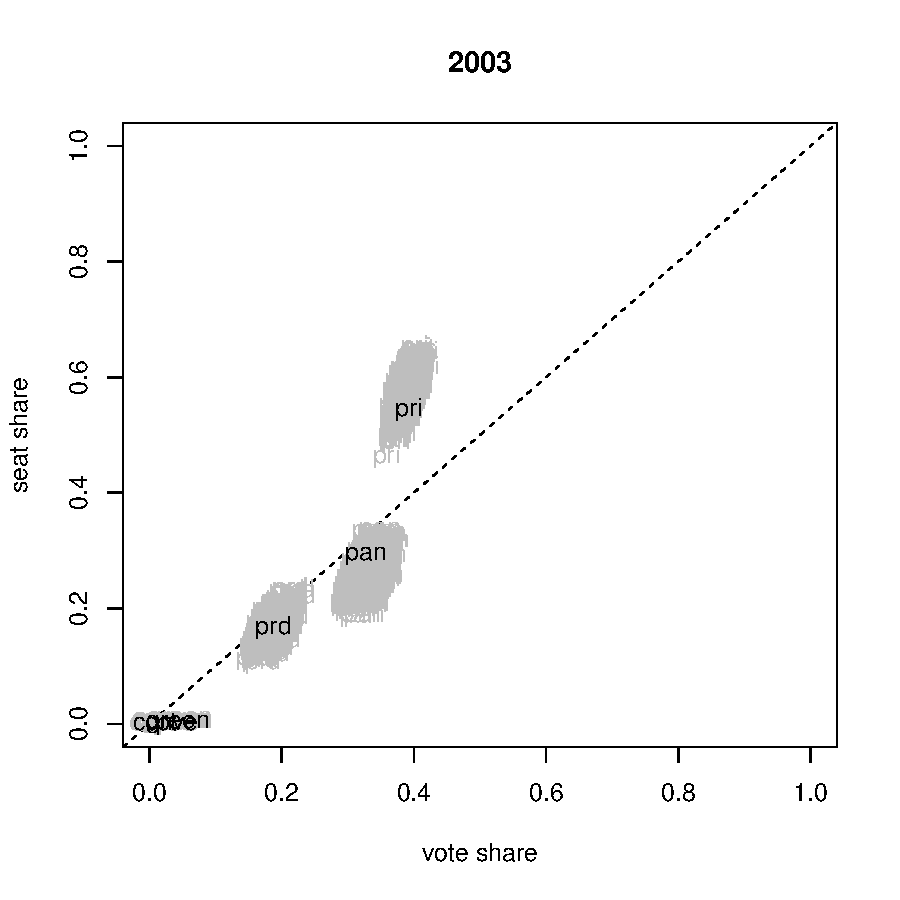
\includegraphics[width=.4\columnwidth]{vs2003.pdf} &
    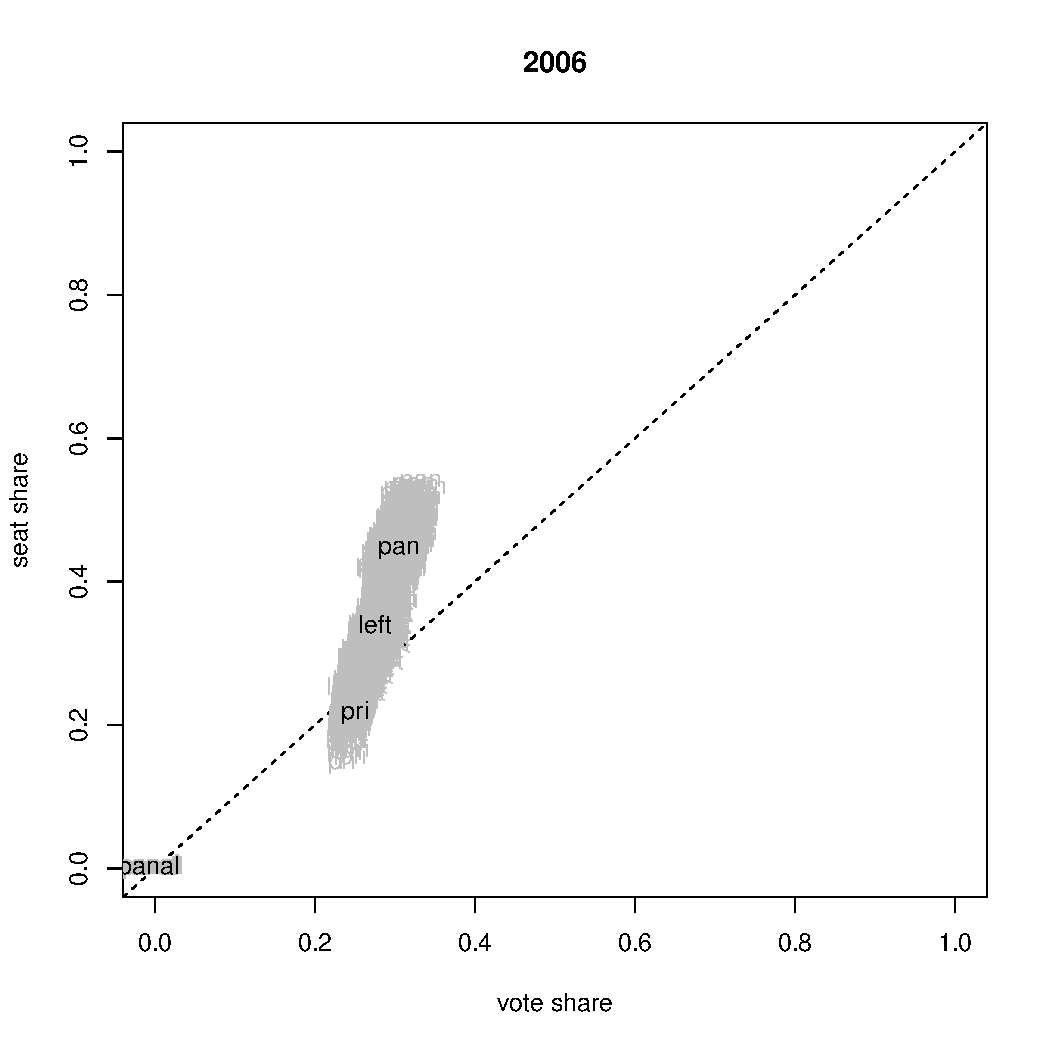
\includegraphics[width=.4\columnwidth]{vs2006.pdf} \\
    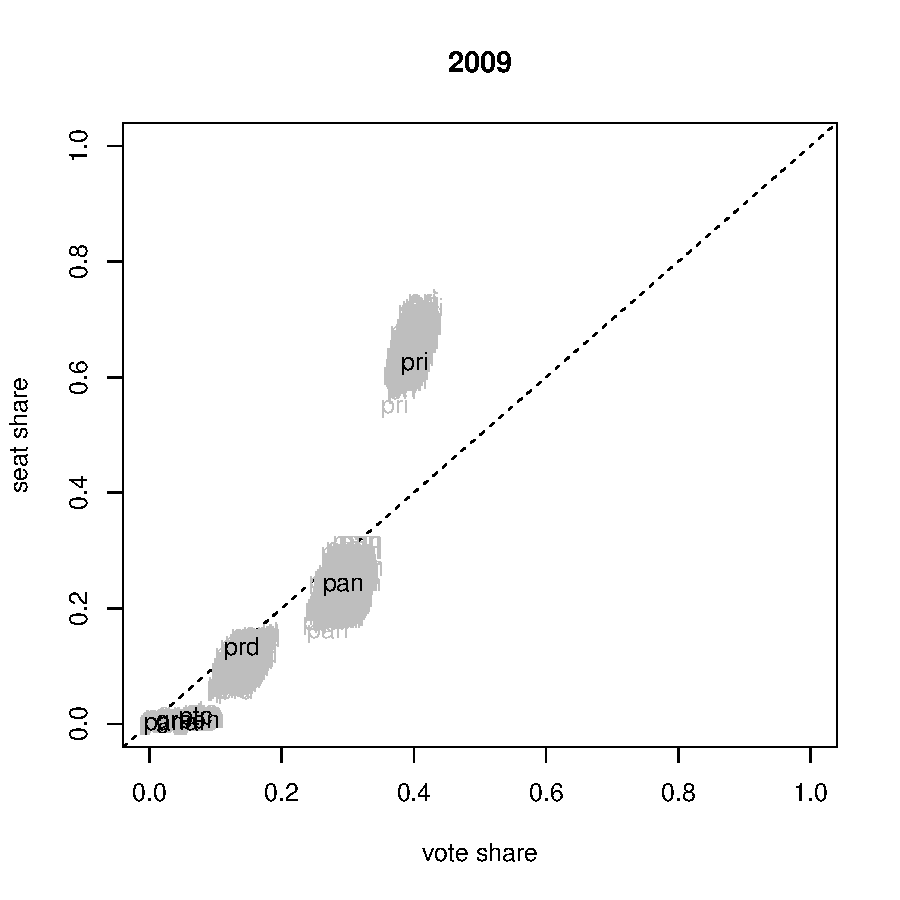
\includegraphics[width=.4\columnwidth]{vs2009.pdf} &
    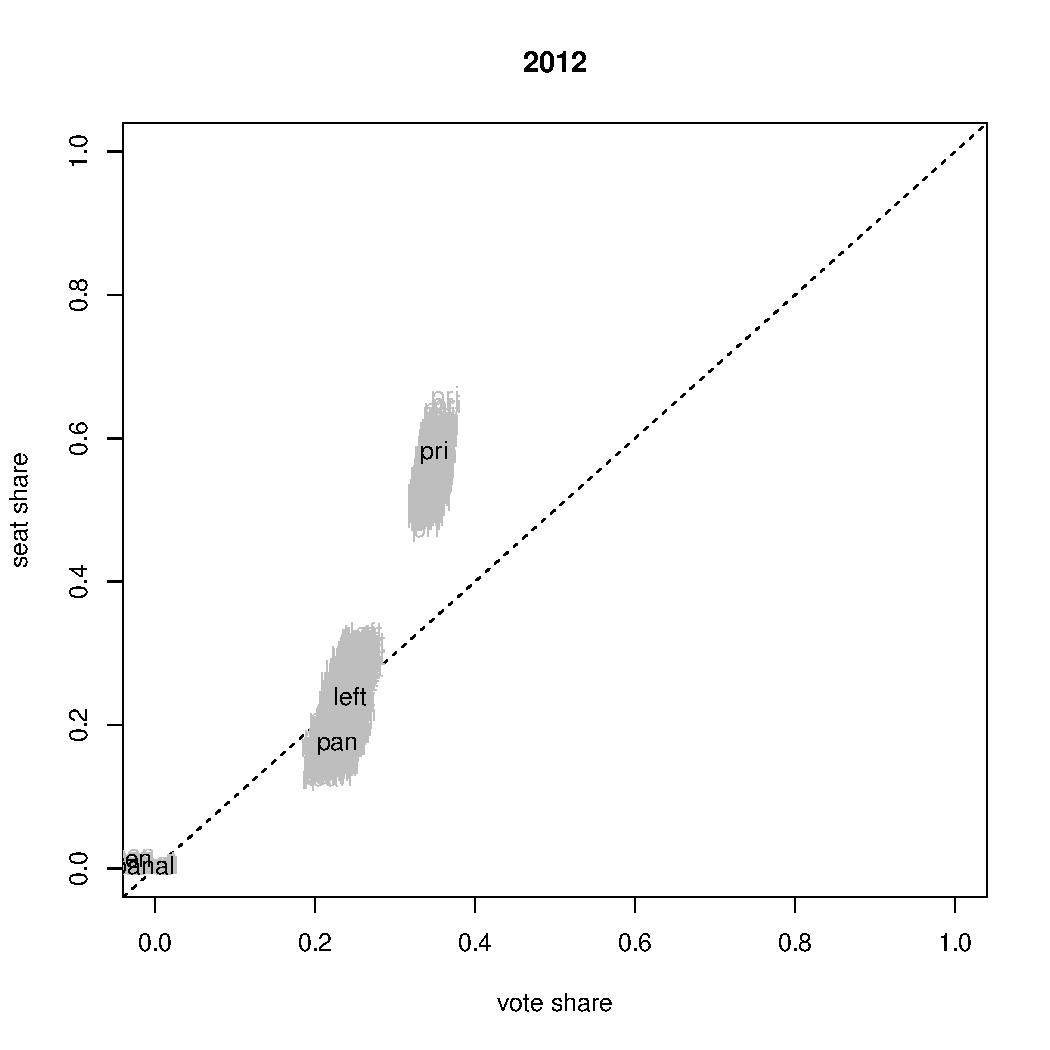
\includegraphics[width=.4\columnwidth]{vs2012.pdf} \\
\end{tabular}
\caption{Votes and plurality seats in four elections. Actual data in black, simulated elections in gray. Source: prepared with data from \url{www.ine.org.mx}.}\label{F:singleYrSeatsVotes}
\end{center}
\end{figure}

Figure \ref{F:singleYrSeatsVotes} presents the output of the simulation process for the Mexico case study that section 4 presents in detail. Observed national votes received and seats won appear as black labels for four consecutive elections. Simulated elections are surrounding clouds of gray labels. These counter-factual predictions are most reliable  near observed points \citep[about $\pm5$ percent,][:fn.\ 8]{linzerSeatVoteElasticity2012}. The single-election approach is not suited for extreme counter-factual prediction \citep[something generally true for any approach,][]{gelman.king.1994EvalElSysRedis}. However, given the challenges with longitudinal studies, this is the best available approach.

% comment [Eric] X +/- 10 percent can be defined as [X-10%,X+10%] or as an interval of range 10% around X---i.e., approx [X-5%,X+5%]. I used the first, but which is kosher?
% comment [Mike] I prefer the latter method. As described in the text I would have assumed the range was [X-5%,X+5%]. If you used the first range, I'd recommend changing the text to $\pm10$

Another technical problem is that parties may not field candidates in all legislative districts. Strategic parties often withdraw in anticipation of a hopeless race. The mixture method handles this issue by considering patterns of district contestation separately. This method does require adjustment when parties form partial coalitions---e.g., when parties A and B field joint candidates in some districts but run against each other in others. This issue occurred in recent Mexican elections, and we address it in greater detail in the next section. 

\section{Mexican C\'amara de Diputados elections}

We demonstrate our procedure through analysis of recent elections of Mexico's lower chamber of Congress. The C\'amara de Diputados has been elected with a mixed-member electoral system for decades. Systems of this nature give voters a direct role in the election of representatives from single-member districts, while additionally using some form proportional representation reduce votes--seats distortions often magnified in plurality systems \citep{shugart.wattenbergIntro2001}. We examine, in isolation, the elections held in the single-member plurality-win districts. We do so because all voting and most campaigning take place in the plurality tier.\footnote{Each voter casts a unique, non-exclusive, pooling vote to choose among candidates in 300 single-member districts with seats allocated by plurality. Votes then transfer to the party to which the candidate originally voted belongs, in order to allocate seats in five second-tier districts of magnitude 40, by closed-list Hare PR, using a 2\% threshold \citep{weldonMixedMemberSys2001}.} 



Some might argue that bias distortions in mixed-member systems are of little, if any, consequence. The proportional representation tier is, after all, specifically designed to compensate for imbalances ensuing from plurality races. Indeed, the PR tier provides conditions for small parties to win seats where they may otherwise be unable to win in single-member districts alone, thus reasonably providing electoral conditions conducive to more than two parties. Yet, bias still has the potential to substantially distort representation in Mexico's mixed-member system. \citet{cox.1997} shows how in single-member districts, election contests tend to devolve into competition between the two leading party's candidates in each district. If systematic partisan bias exists, trailing parties that do not field one of the top two candidates will find themselves disadvantaged in the PR tier as their voters abandon their candidates to select one of the top two candidates most likely to win the district election. Alternatively, bias may arise when a party systematically finds its supporters are concentrated in oversized, electorally uncompetitive, low turnout districts.\footnote{Compensating \emph{parties} bears relation to, but is not the same as, compensating \emph{citizens} of over-populated districts. Keeping these compensations distinct is important. Much of the evidence presented here, as in the scholarly literature, deals with party votes to seats ratios. From the normative standpoint, however, it is the `one person, one vote' principle---one of Dahl's \citeyearpar{dahl.1972} preconditions of democratic government---that malapportionment antagonizes, and party compensation is not designed to redress this imbalance. The exception would be a system with perfectly district-based parties, where measures to achieve party proportionality are, in fact, compensations for the district citizenry only. Shifts away from fully local parties, towards party nationalization, and party compensation stop accruing to citizens of the underrepresented districts only.} 

We suspect strong distortions of vote shares into seat shares exist in Mexico's electoral system, which manifest in partisan bias such as is regularly found in other single-member plurality systems. \citet{marquez2014biasBlog}, using a multi-election approach to analyze votes and seats won over two decades, uncover a degree of responsivity characteristic of plurality systems and substantive partisan bias against the PAN. Our proposed procedure offers a way to answer questions of theoretical interest by showing the contributions of malapportionment, distributional, and turnout to bias in each election. 

%comment [Mike] I can imagine a reviewer comment along the lines: how would the overall seats to votes appear if hypothetically there were no bias from any of three sources?

Mexico held its first free and fair congressional election in 1997. In advance of this election, the government delegated election management to a newly-appointed independent board \citep[the Federal Electoral Institute IFE, see][]{lujambio.vives.2008}. Closer inspection of the board's structure and process reveals how, in practice, it is a power-sharing agent of the major congressional parties \citep{estevez.magar.rosas.2008}. Systematic partisan segmentation of the board provides evidence of major-party influence in election regulation. This influence extends to redistricting, as the electoral board was charged with drawing C\'amara de Diputados districts. 

Mexico's election management board drew district boundaries using machine-assisted mapping in 1997 and 2006. New district boundaries were proposed in 2015, but the board rejected implementation of this plan when redistricting became conflated with a broader package of electoral reforms. We explore all the board's proposed redistricting plans in our analysis, including the recently rejected map. We examine Diputado elections concurrent with the presidential races of 2006 and 2012, and the midterm elections of 2003 and 2009. Electoral rules were unchanged, but district maps changed: 2003 used one map (we call it the ``1997 map'' because it was inaugurated that year), the other elections were conducted using the 2006 map. 

We compile data from IFE's official election returns, available at \url{www.ine.mx}. \footnote{Upon publication, all data and code for our analysis will be made available through a durable publicly accessible archive.} Our analysis requires district-level data to simulate national vote and seat shares by party. We further disaggregate secci\'on-level returns to re-aggregate votes into hypothetical district maps as part of our analysis.\footnote{\emph{Secciones electorales} are analogous to U.S.\ census tracts. Median secci\'on population in the 2010 census was 1,280, with a maximum at 79,232; median tract population in the 2010 census was 3,995, with a maximum at 37,452. The 1997, 2006, and 2015 maps (kindly shared by IFE's cartography department) relate more than sixty-six thousand secciones, the basic units for district cartography, to 300 congressional districts. This made reconstitution of hypothetical election outcomes in the period possible.} Party district-level vote shares are defined as the number of votes won divided by a district's effective vote; which is a district's vote total minus voided ballots, votes for write-in candidates, and votes for parties failing to clear the 2\% threshold nationwide.\footnote{\citet[][:fn. 4]{linzerSeatVoteElasticity2012} recommends likewise. Five parties were thus removed in 2003 (PAS, PSN, FC, MP, and PLM) and one in 2006 (ASDC).} Analysis also requires district-level population figures (and, for hypothetical map analysis, secci\'on-level populations as well). Years 2000 and 2010 census data, and the 2005 population count were compiled from data prepared by Mexico's census bureau (INEGI) for the purpose of redistricting. Linear 2000--05 and 2005--10 projections provide point estimates of between-census election-year populations. 

Seven parties are included in our analysis. Three are major parties, with vote shares above 15\% (albeit volatile, as seen in Figure \ref{F:singleYrSeatsVotes}): the right-of-center National Action Party (PAN) that controlled the presidency throughout the period; the formerly hegemonic Institutional Revolutionary Party (PRI); and the left-of-center Democratic Revolution Party (PRD). Minor parties with vote shares slightly above the 2\% threshold complete the slate: the Green (personalistic), the PANAL (close to the teachers' union), Convergencia (personalistic), and PT (personalistic of Maoist bend). Major parties contested every district systematically, but often in pre-election coalitions. The PRD fielded common candidates with Convergencia and the PT nationwide in 2006 and in 2012 (they are labeled `left' in plots); the PRI forged a coalition with the Green in 2003 and 2006; and Convergencia and PT ran together in 2009. 

Partial PRI--Green coalitions took place in 2009 and 2012---the partners fielded joint candidates in one-fifth and in two-thirds of the districts, respectively, but competed against each other in the remainder. Partial coalitions complicate national votes and seats aggregation. The option of computing separate aggregates for PRI, for Green, and for PRI--Green is attractive for describing the situation faithfully, but we decided against this approach. Notably, the PRI would wrongly appear as fielding no candidates in numerous districts, thereby artificially underestimating its true electoral strength. We opted instead to exploit the coalition partners' size asymmetry by considering PRI--Green votes won in tandem as if the PRI won these contents solo---thus contributing returns in every district for the national aggregate (it appears as `pri' in plots). While this approach is far from satisfactory (the Green is the largest and most successful of minor parties, it may soon qualify as major) the solution is practical, and credits the fact that the partners never failed to team electorally to some degree throughout the period. 

\section{One Mexican, one vote?}

% [Micah] Since they are projections, these should be accompanied by a measure of uncertainty. The uncertainty should be represented in this graph (error regions) or in the appendix.
% [Eric] I searched for a confidence interval in the census' population figures (they are estimates, after all) but could find none. These are, presumably, necessary to achieve Micah's suggestion.

Mexico is familiar with malapportionment. Districts of unequal population are common practice in Mexico despite a set of clear quantitative redistricting criteria that since 1997 includes population equality \citep{altman.magar.mcd.trelles2014apsa}. In practice, Mexican parties in general, and the election board in particular, have been tolerant of malapportionment. Malapportionment typically occurs in electoral systems around the world when apportionment formulas assign districts to geographic units, such as states, according to their population. Unequal-sized districts result when the geographic units' populations are not neatly divided by the number of seats. An additional source of malapportionment exists in Mexico: a time lag between the conduct of the national census and redistricting, what \citet{JohnstonCreepingMal} calls ``creeping malapportionment.'' Mexico's constitution mandates the use of the census for redistricting, but the government has no obligation to redistrict as soon as population data become available. As a consequence, six or more years have routinely passed between a new census and the time new district boundaries are inaugurated. Rectifying malapportionment is, ironically, an essential representational justification to periodically redistrict. Yet, substantial malapportionment exists  even as a new map is implemented. 

% PLOT PREPARED IN RED.R
\begin{figure}
\centering 
  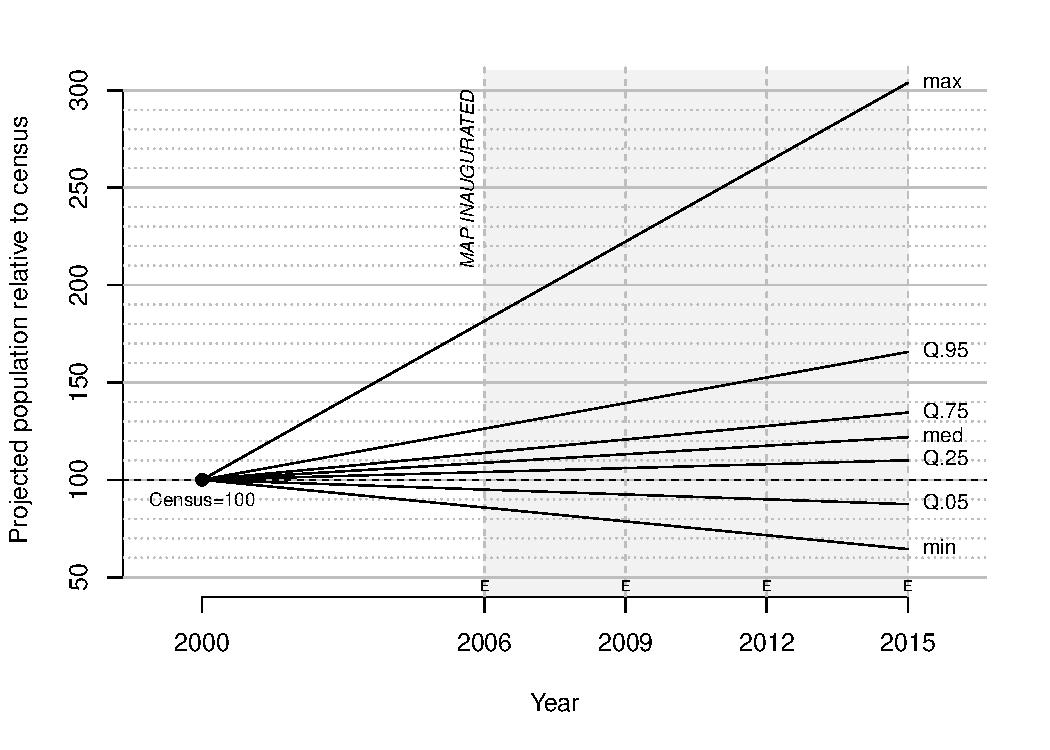
\includegraphics[width=.8\columnwidth]{disRelPopProj2006map.pdf} 
  \caption{The 2006 map and demographic change. Plotted population projections relied on the 2000--2010 censuses rate of change (see text for details). Letters \textsc{e} in the horizontal axis indicate elections using this map. Source: prepared with data from \url{www.inegi.org.mx} and \url{www.ine.mx}.}\label{F:disRelPop2006map}
\end{figure}

Figure \ref{F:disRelPop2006map} illustrates how creeping malapportionment affects Mexico's redistricting. We linearly project inter-census populations to estimate yearly district growth.\footnote{More precisely, the 2000--2005 rate of growth was used before year 2006, and the 2005--2010 rate afterwards. Population projections for different maps were done after secci\'on census populations had been aggregated into actual or hypothetical districts. Performing linear projection on secciones before any aggregation might have been preferable (because they are much smaller geographic units), but a fair amount of over-populated secciones are routinely split into new ones between elections, complicating the projection exercise.} Compared to the 2000 census, projected district populations in 2006 are off by 9.7\% in absolute value on average, with a standard deviation of 10.6\%. With one additional year away from the reference census, the 1997 map had even less success achieving proper apportionment at implementation. Indexing 2000 census district populations at 100, as the figure does, reveals how different the most demographically dynamic units were on paper and in reality. The fastest-growing district was 88\% larger in 2006 than what census data otherwise suggested (the line labeled `max'). The district shedding most population was 16\% smaller (the `min' line). These are outliers, but central tendencies reflect sizable lags as well. The inter-quartile range (lines Q.25 and Q.75) covered 1\%--13\% above census in the 2006 election, and expanded to 4\%--20\%, 7\%--27\%, and 10\%--35\% in the three subsequent Diputado elections using the same map.
 

%One year closer to census makes a huge difference, as the abandoned map for 2015 reveals (although this is probably compounded with a less dynamic demography): the dotted vertical line at year 2013 reports how the new plan might have looked, had it been adopted. 

The lag between census and redistricting is, of course, not the only cause of malapportionment. Small deviations around mean district population are almost always unavoidable simply because districts usually cannot slice populations so finely to create perfect population balance between districts. Courts in the U.S.\ have struck down new U.S. House district maps bearing less than 1\% differences within states without proper justification \citep{tuckerApportionment.1985}. U.S. redistricting authorities generally view \emph{de minimus} population deviations of as little as one or zero persons between congressional districts as desirable to inoculate against litigation---although larger differences are permitted for elections at other levels of government. In stark contrast, Mexico's electoral board has permitted deviations between 10\% (in 2006) and 15\% (in 1997 and 2015) above or below mean state district size \citep{lujambio.vives.2008,trelles.mtz.polygob2012}. The greater population deviation is designed to give deference to competing redistricting criteria, such as minimizing the number of municipalities that must be partitioned into two (or more) federal districts and keeping within the same district municipalities with large indigenous populations.\footnote{The rationale is minority protection. In practice, however, there is no consideration of primordial differences between contiguous, and possibly antagonistic indigenous communities---all fall in the `indigenous' category, and are grouped in one congressional district \citep{sonnleitner.elsCps2012}. The case of Arizona's Hopi and Navajo tribes is an example where a redistricting authority made a conscious effort to segregate antagonistic tribes \citep{stephanopoulos.redisCommunity2012}.} The representational effect is substantial: two districts with populations exactly at the bounds of the legal spread afford citizens at the bottom bound one-third more representation in Congress than those at the top. 

Creeping malapportionment and bureaucratic discretion potentially compound to produce considerable malapportionment in Mexico's congressional districts. We examine how malapportionment distorts representation, following \citet{ansolabehere.gerber.snyderCourtRedis2002}. We measure a district's relative representation index as $RRI = \frac{1/\text{district size}}{300/\text{national population}}$, where the numerator is the number of diputado seats per person in the district and the denominator is the average number of diputado seats per person nationwide (300 is the number plurality seats). A district with unity index value has representation matching the `one person, one vote' ideal perfectly. Values above one indicate over-representation, values below one under-representation, and the measure is continuous. An example shows how the index is interpreted. The 3rd district of Aguascalientes in 2012 had about 306,000 inhabitants, and 300 divided by Mexico's population was about 387,000. So the district in question had 26\% more representation than the national average, for an index value of 1.26. As above, we used population projections to compute $RRI$s.

The percentiles corresponding to $RRI$s at .85 and 1.15 (the bounds of the board's $\pm15\%$ tolerance range) in 2006 were 10 and 87, respectively, implying that $10+100-87=23\%$ of districts exceeded IFE's discretionary malapportionment range in the map's inaugural year, as caused by the census lag.\footnote{This is not entirely accurate, as the $\pm15$ range is in reference to average state population \citep[not average national population, analyzed here, see][]{altman.magar.mcd.trelles2014apsa}. The percentiles using state population $RRI$s are .06 and .89, or 17 percent out-of-legal-range districts in 2006.} By 2012, more than one-third districts were outside the tolerance range, and by 2015 just shy of two-fifths were outside the tolerance range. As the U.S. Supreme Court found in the 1960's, using antiquated population data impairs drawing equal-sized district boundaries and substantially distorts representation. 

% USED CODE IN RED.R TO DO THIS PLOT
\begin{figure}
\begin{center}
    % 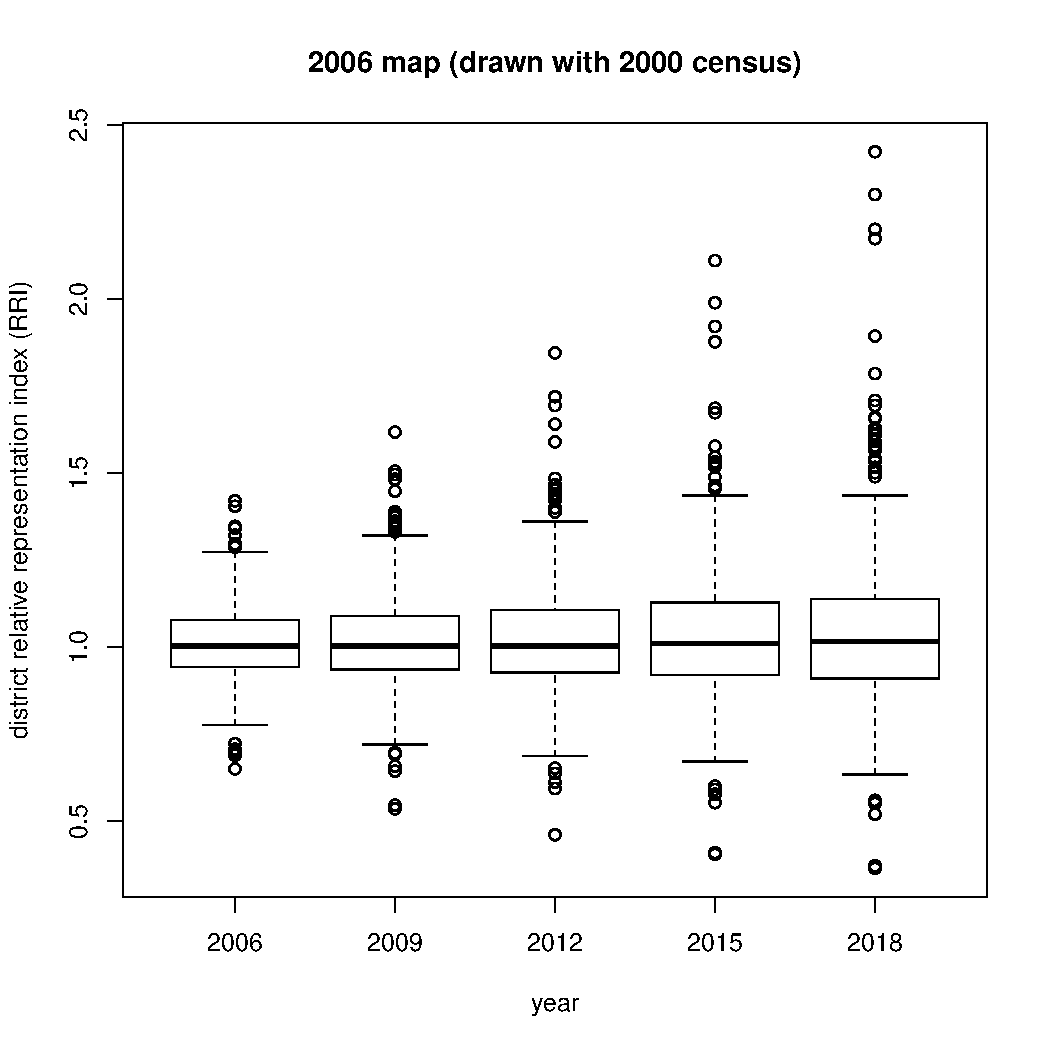
\includegraphics[width=.65\columnwidth]{rris0618d0.pdf} \\ 
    % 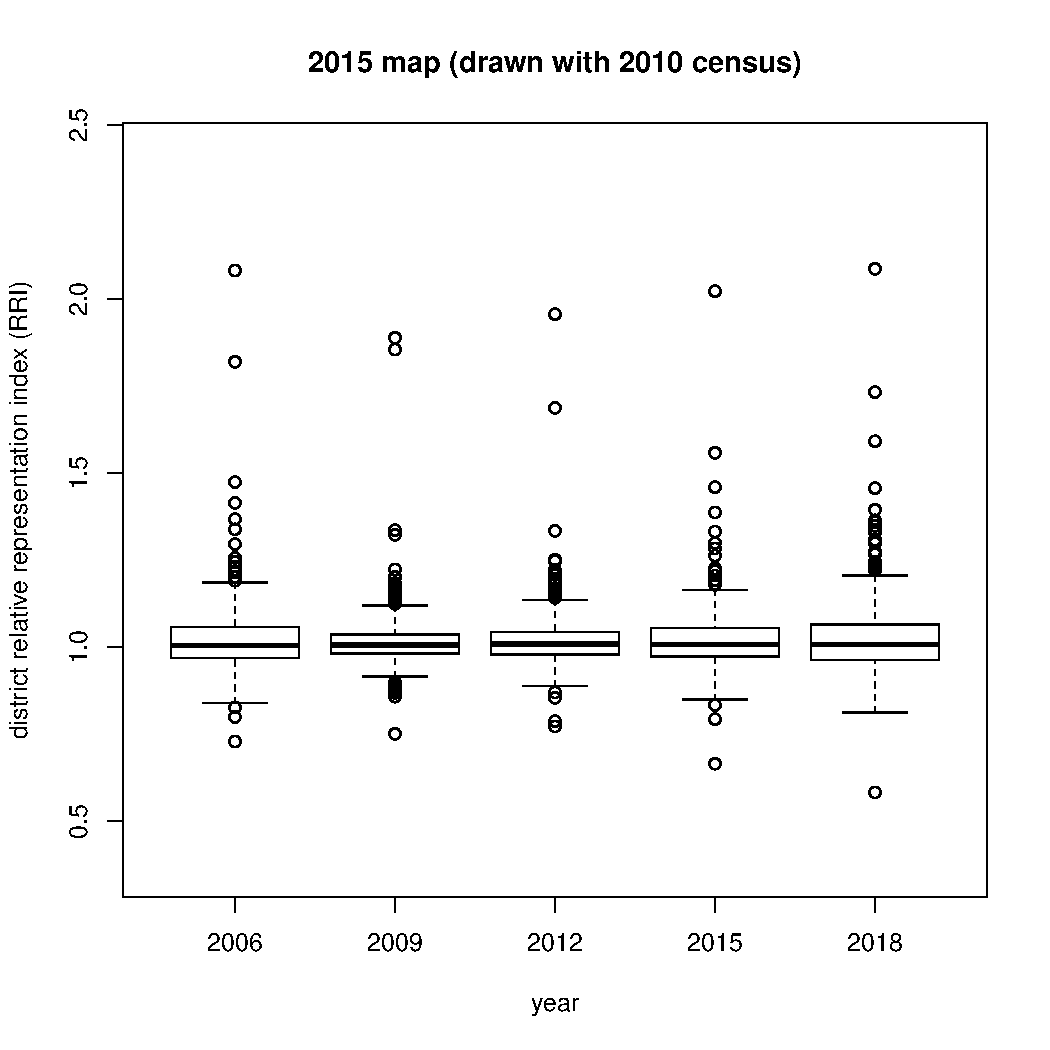
\includegraphics[width=.65\columnwidth]{rris0618d3.pdf}  
%\begin{tabular}{cc}
    %(a) & (b) \\ 
    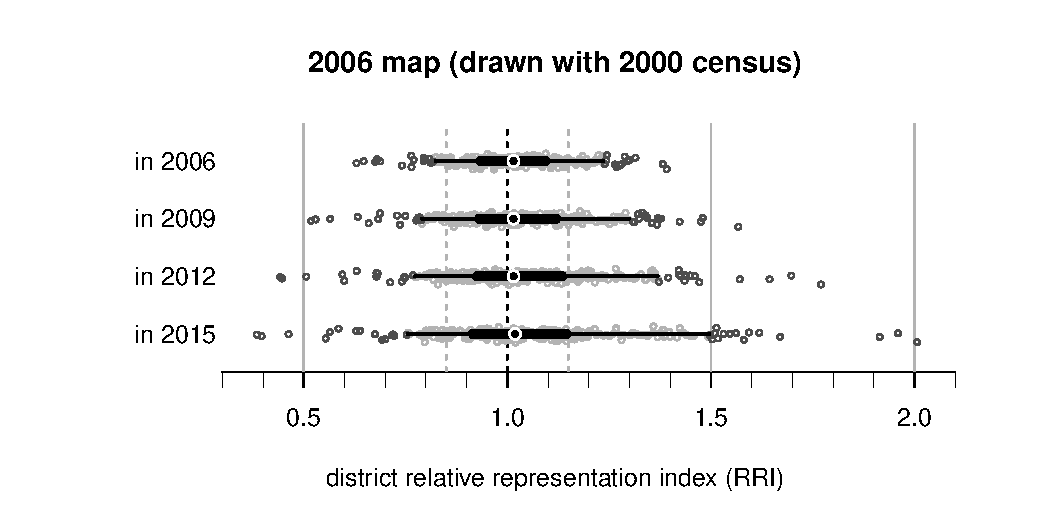
\includegraphics[width=.65\columnwidth]{rrin0615d0.pdf} \\
    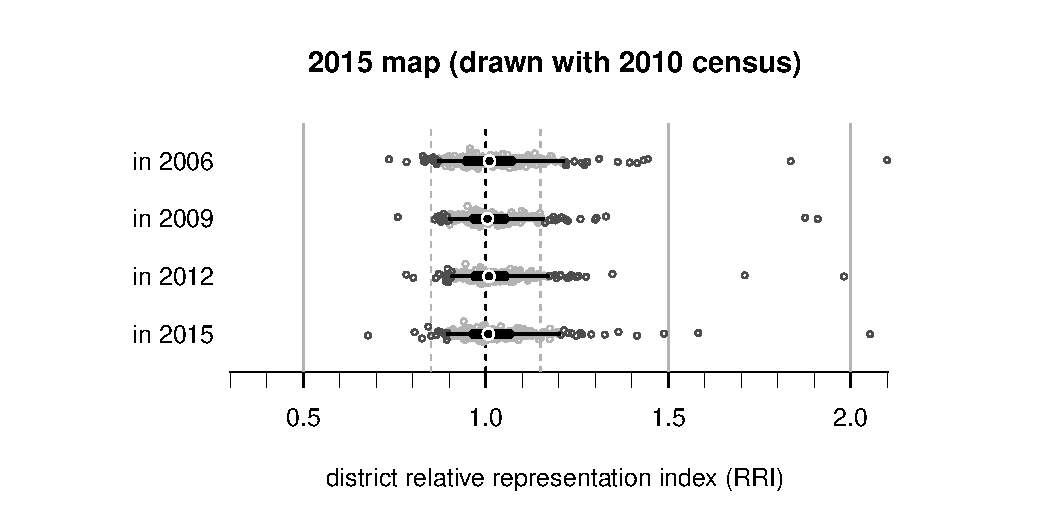
\includegraphics[width=.65\columnwidth]{rrin0615d3.pdf} \\
%\end{tabular}
\caption{Representation in four elections and two maps. Panels portray (top) the status quo and (bottom) the hypothetical maps. Finer horizontal lines connect the 5th and 95th percentiles, thicker lines the quartiles, and white circles indicate the median. Points are districts.}\label{F:malapp}
\end{center}
\end{figure}

Figure \ref{F:malapp} summarizes the effects of creeping and discretionary malapportionment in representation. Vertical dashed lines in gray mark the board's tolerance band, which has been amply and systematically surpassed. Consider the top plot, portraying the status quo map, first. Each point represents one district. The fine horizontal line connects the $RRI$ values corresponding to the 5th and 95th percentiles---both well outside the tolerance range, since the map's inception. The thick horizontal line is the inter-quartile range, not far from covering the full tolerance range by 2012 (if it did, half the districts would be off-range). For the 2015 midterm congressional election (not analyzed because data has not been published), citizens in the plot's right-most districts (in central Monterrey and two in battered Ju\'arez) will be worth \emph{four times more} in Congress than citizens in the left-most districts (one each in suburban Monterrey and Mexico City, the other in Canc\'un). In matters politic, citizens at one quartile will be worth nearly twice as much as those at the other quartile. 

The bottom plot is a counterfactual, analyzing the map that IFE proposed for the 2015 election, but did not formally adopt. It is quite clear that, even if outliers remained upon implementation, this hypothetical map would have represented Mexicans much better than the status quo (note the narrower horizontal lines). Taking this thought experiment further, it is possible to aggregate section-level population projections for 2009 into the hypothetical map to assess its performance in the year closest to the reference census. Like fish, fresh demographic information is still a must: a handful of the proposed districts in that year are still outside the tolerance band. 

% comment [Mike] I rewrote this to argue that the new plan still had creeping malapportionment. Please check.
% comment [Eric] "rejected by C\'amara de Diputados" dropped. 

The evidence is unambiguous: malapportionment in Mexico is systematic and substantial, a consequence of using outdated census data and of balancing population equality against other criteria that permits unequal district populations.\footnote{The comparative survey by \citet{snyder.samuelsMalapp2004} ranked Mexico among well-apportioned cases. The measure reported is for the 1997 map, but no guidance is offered about the population figures used in denominators. We suspect his reliance---as the board did then and still does now---on raw 1990 census data, severely underestimated Mexico's malapportionment.} 

\section{Results}

We now turn to estimating overall bias and its components. We fit equation \ref{E:kingMulti} using MCMC estimation to generate overall bias and responsiveness estimates.\footnote{\citet{gelman.hill.2007} is a comprehensive introduction to MCMC estimation. For each vote operationalization ($v$, $\bar{v}$, and $\bar{w}$), three chains were iterated 100 thousand times, taking every 500th observation of the last 50 thousand to sample the posterior distribution. The Gelman--Hill $\hat{R} \approx 1$, evidence that the chains had reached a steady state. Convergence was also inspected visually in chain trace plots of each of the model's parameters. Estimation performed with open-source software \texttt{Jags} \citep{jags.cite}, implemented in \texttt{R} \citep{r.cite} with library \texttt{R2jags} \citep{r.r2jags}. Data and commented code to replicate the analysis will be posted on-line upon publication.} The responsiveness parameter is of secondary interest here, but useful to assess model fit. Judging the 90\% Bayesian confidence intervals (i.e., the 5th to 95th percentile range of $\hat{\rho}$'s posterior sample) reveals sizable shifts in the estimate between congressional elections: from a low of $[2.2,2.4]$ in 2012 to a high of $[2.6,3.0]$ in 2006. The large-party premium of recent Mexican plurality congressional races is about one-sixth smaller than the power of the putative cube law of plurality elections \citep{taagepera.CubeLaw.1973}. 

\begin{figure}
\begin{center}
  % \begin{tabular}{cc}
  %   (a) & (b) \\
  %   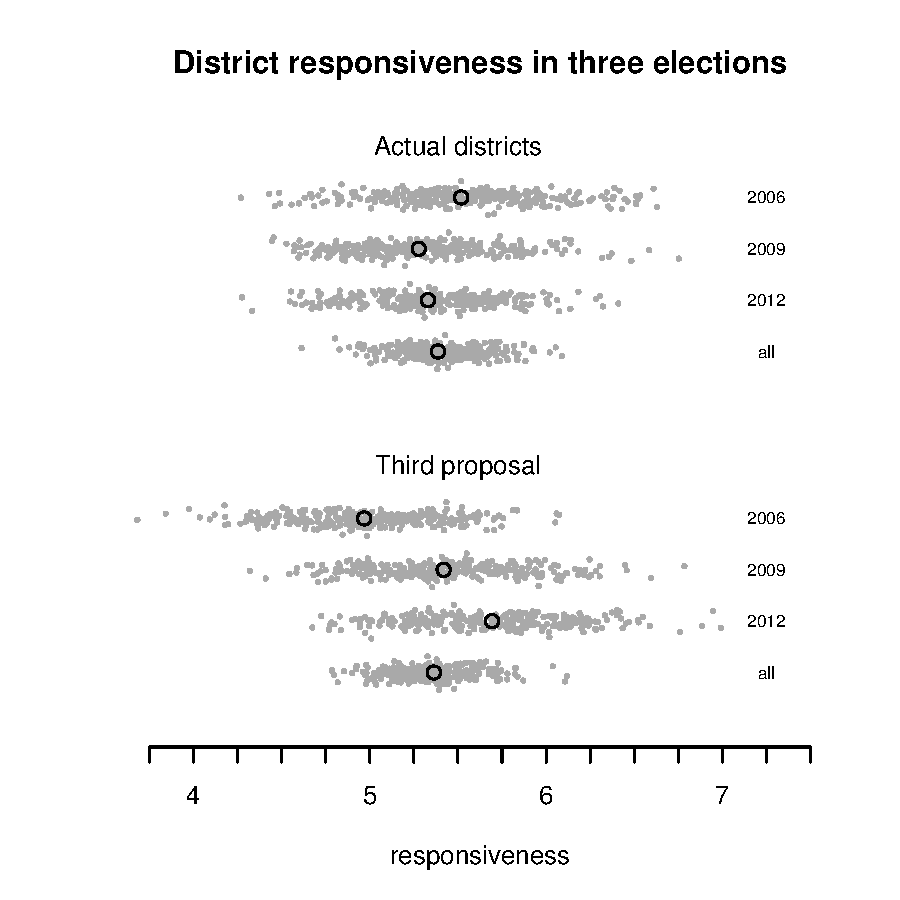
\includegraphics[width=.45\columnwidth]{resp200612s0s3.pdf} &
  %   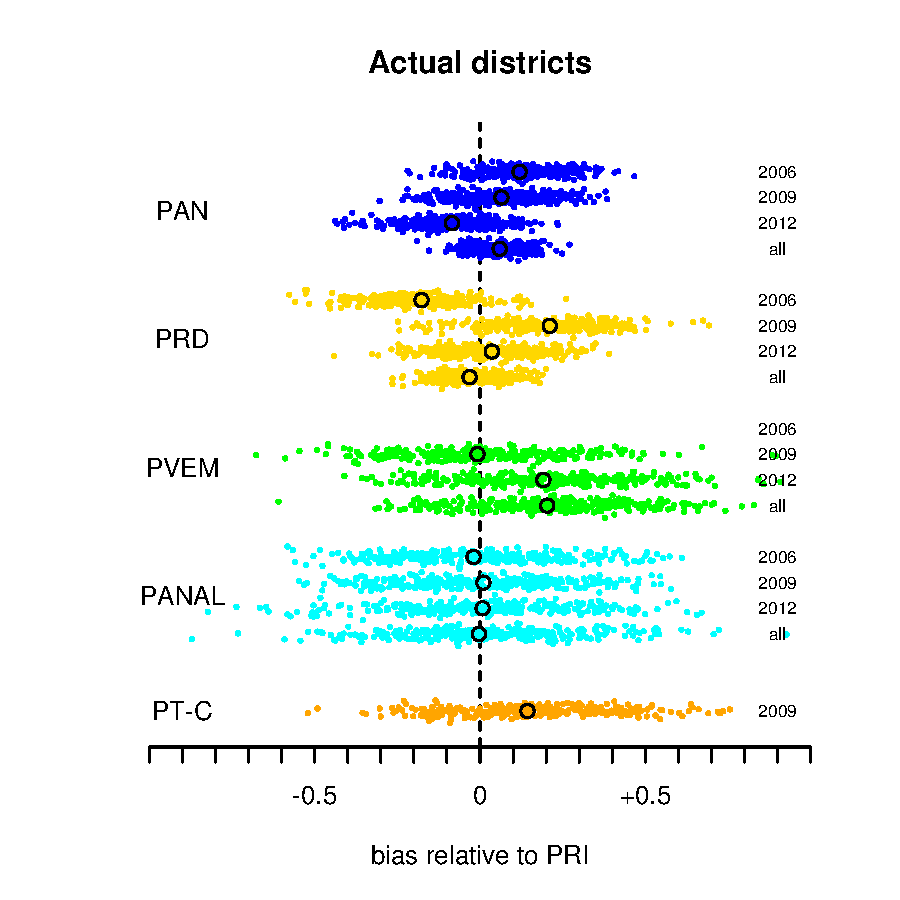
\includegraphics[width=.45\columnwidth]{bias200612s0.pdf} \\
  %   (c) & (d) \\
  %   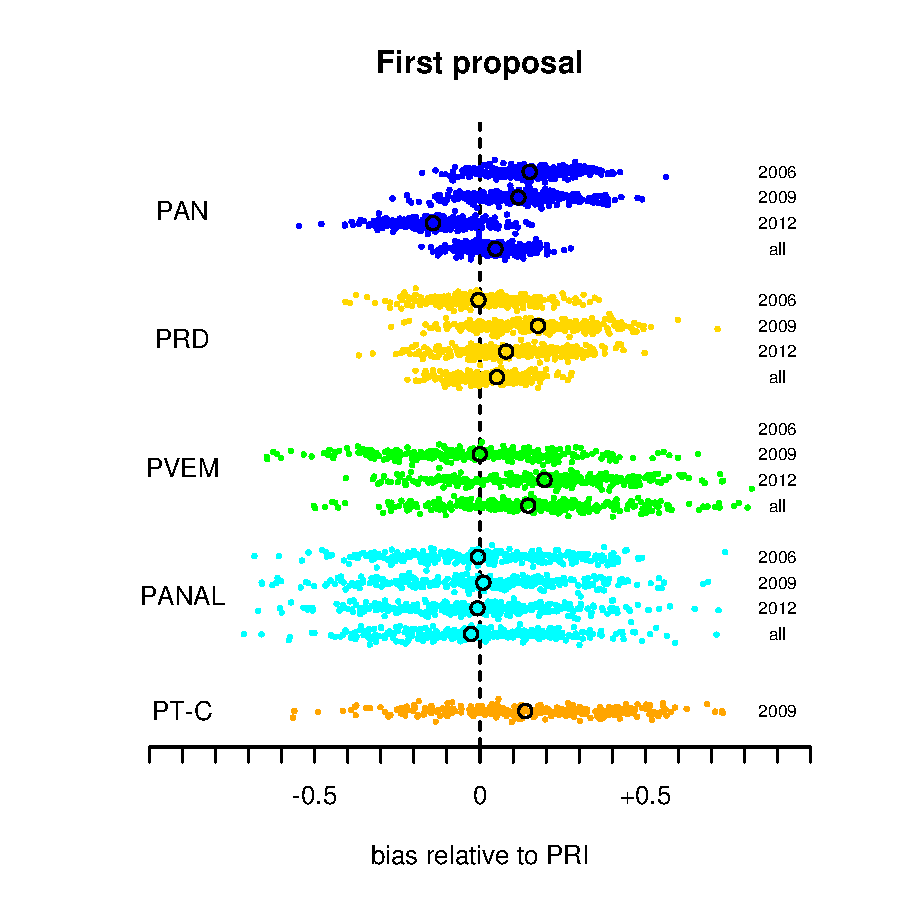
\includegraphics[width=.45\columnwidth]{bias200612s1.pdf} &
  %   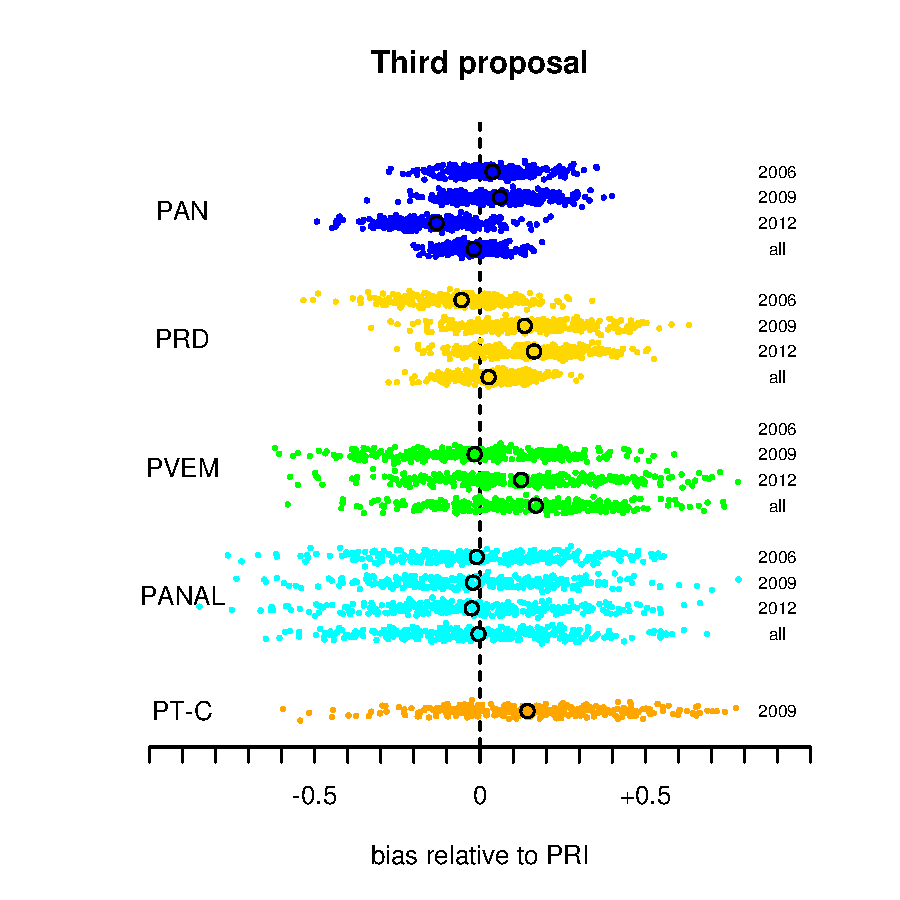
\includegraphics[width=.45\columnwidth]{bias200612s3.pdf} 
  % \end{tabular}
  % \begin{tabular}{cc}
  %   \mc{2}{c}{(a)} \\
  %   \mc{2}{c}{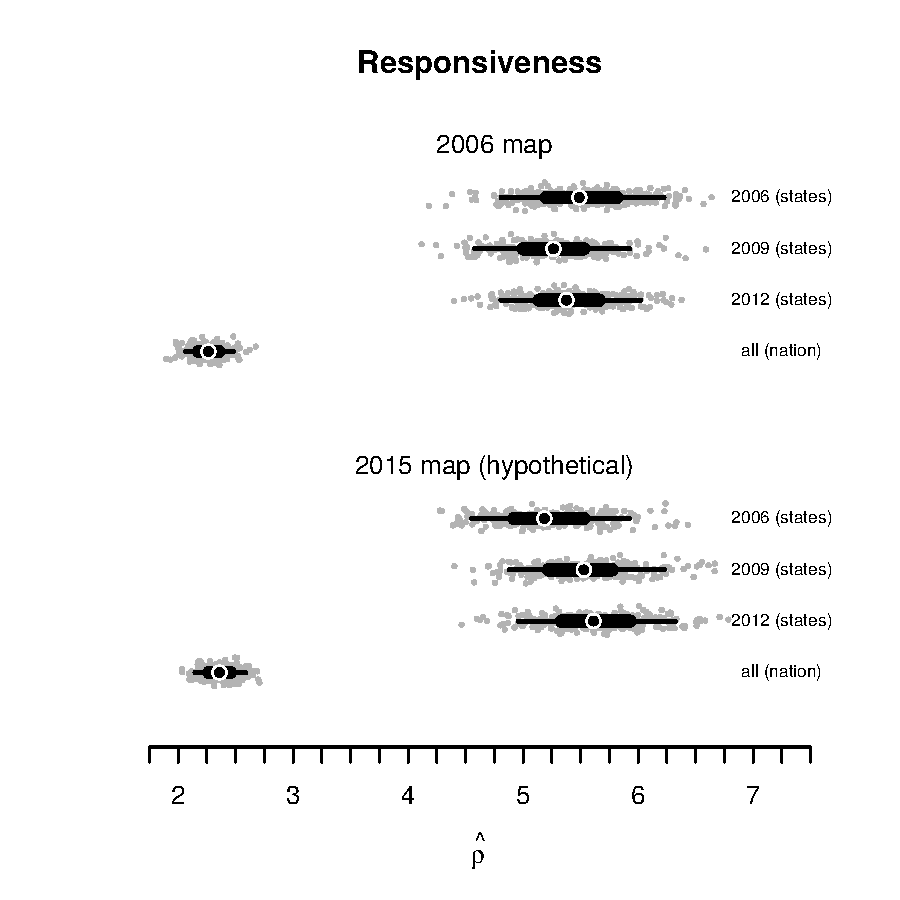
\includegraphics[width=.5\columnwidth]{resp200612s0s3R.pdf}} \\
  %   (b) & (c) \\
  %   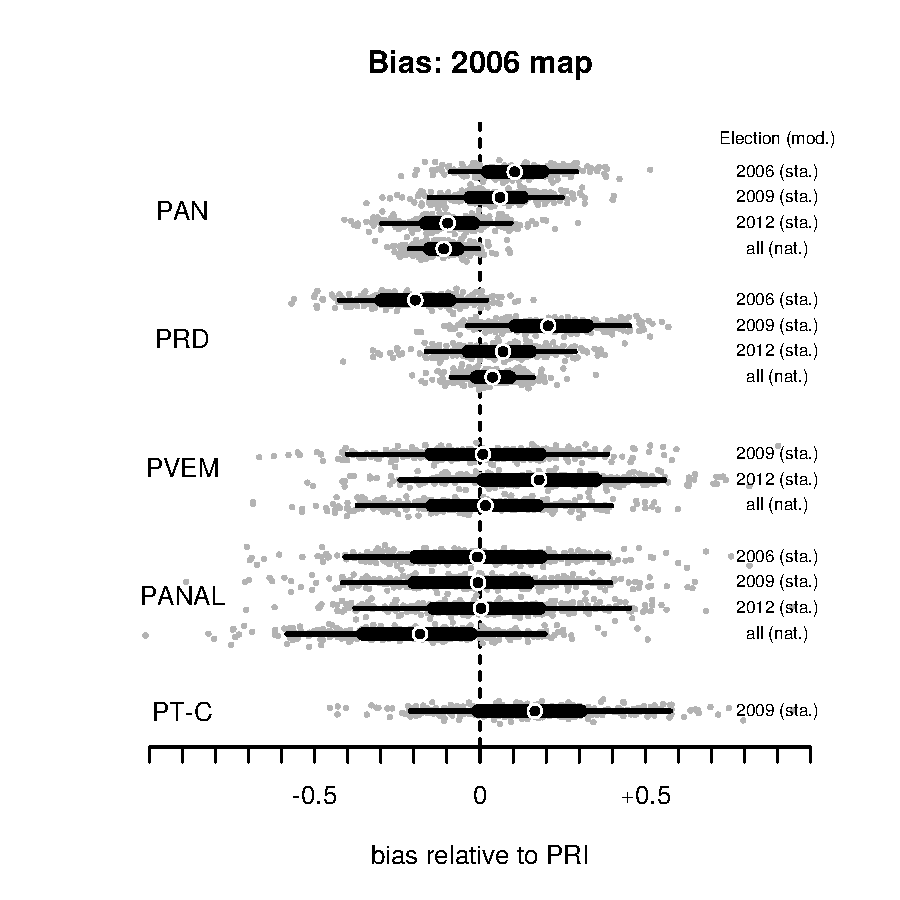
\includegraphics[width=.5\columnwidth]{bias200612s0R.pdf} &
  %   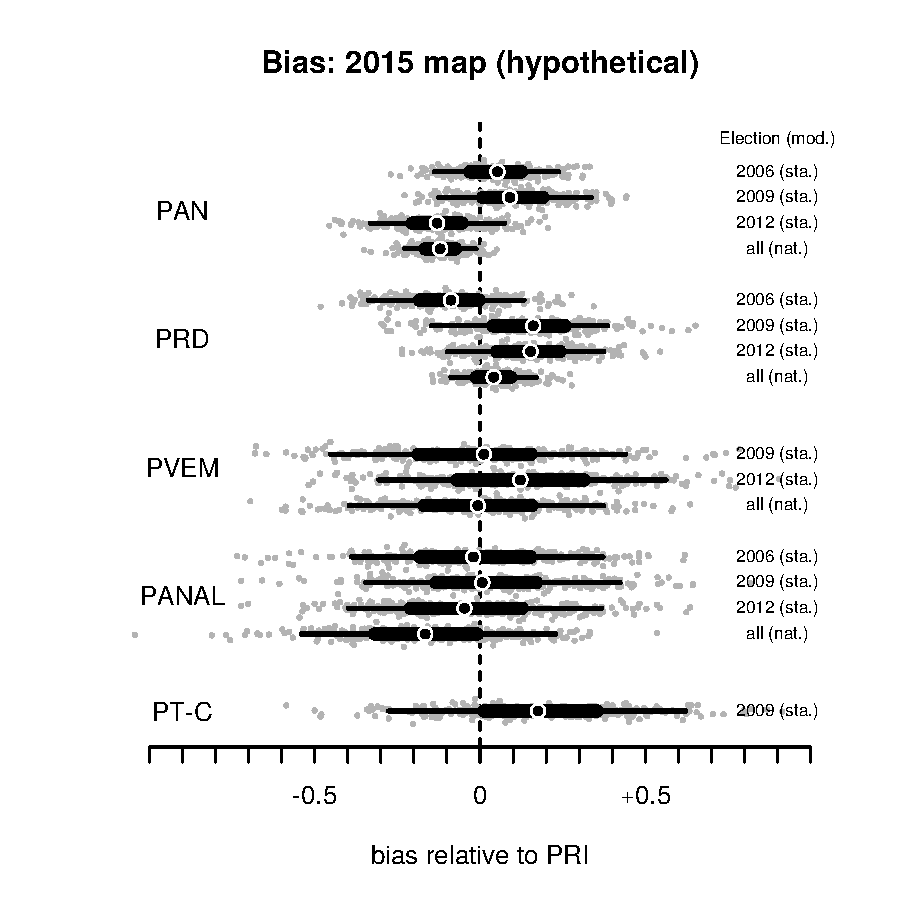
\includegraphics[width=.5\columnwidth]{bias200612s3R.pdf} 
  % \end{tabular}
    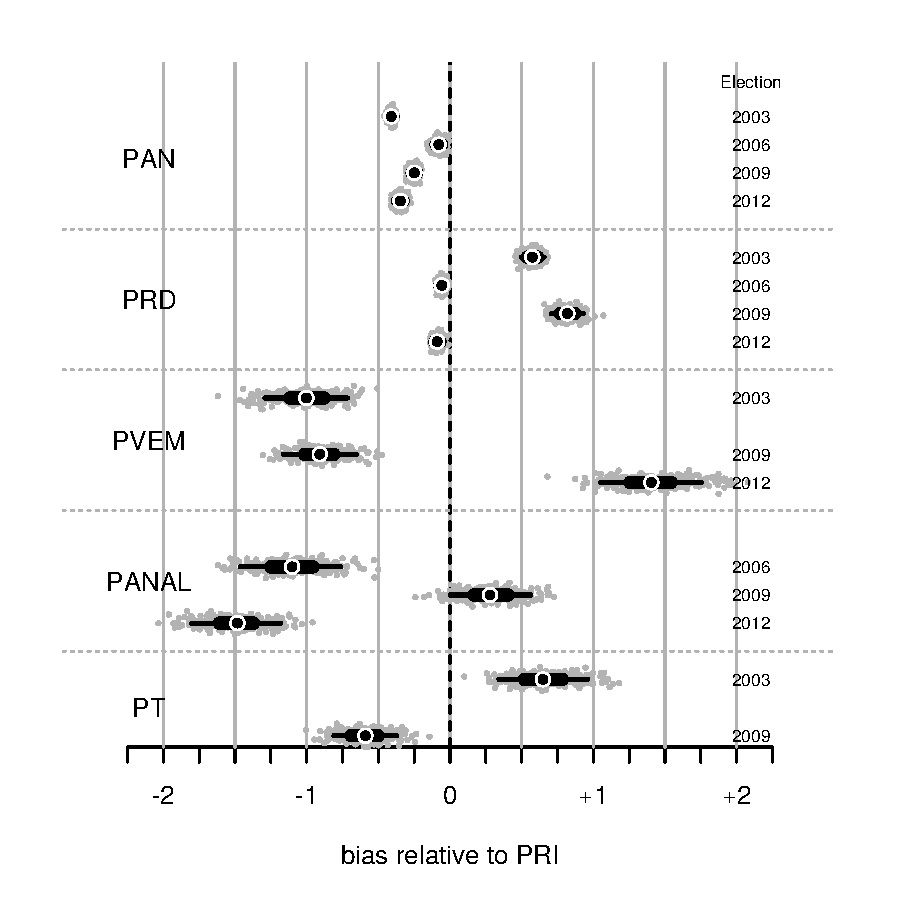
\includegraphics[width=.9\columnwidth]{bias200612d0R.pdf} 
  \caption{Raw partisan bias in four elections. The plot describes the posterior samples (small gray points) of estimated parameters $\hat{\lambda_p}$ for five parties. Some parties did not run in some years. Finer horizontal black lines connect the 5th and 95th percentile values of the posterior sample, thicker lines the quartiles, and white circles indicate the median value.}\label{F:posterior_s0s3}
\end{center}
\end{figure}

% [eric] re-read up to here prior to Oax conf

The raw partisan bias estimates (i.e., the $\lambda_p^v$ parameters) are of direct interest to our investigation. Figure \ref{F:posterior_s0s3} summarizes posterior samples for different parties. We choose the PRI as the reference category and therefore express partisan bias measures relative to the reference (it is for this reason the PRI is absent from the figure). Recall that a negative estimate for a given party is evidence of bias against that party relative to the PRI. Several patterns are noteworthy. Estimate precision (i.e., how concentrated the posterior cloud appears) is consistently higher for major parties than for minor parties (this is true for Convergencia as well, excluded from the plot to save space). Among major parties, the PAN's estimates are the most precise with variation around the median posterior value (taken as the point estimate) nearly indistinguishable at the chosen scale every year. The PRD's estimates are slightly less precise in midterm elections (2003 and 2009) than in presidential election years.  

The size and polarity of the bias estimates reveal important party differences. The PAN experienced negative, albeit small partisan bias vis-\`a-vis the PRI in every year observed. Leaving aside the question of how meaningful the estimated quantities are---we analyze swing ratios below---the near exception was 2006, when the tiny estimate's cloud slightly overlaps with the vertical line at zero. In contrast, the PRD experienced favorable and substantive bias relative to the PRI in some years but not in others. Paradoxically, partisan bias in favor of the leftist PRD is a mirror image of its electoral fortunes: bias vanished when its candidates for Congress rode L\'opez Obrador's presidential campaign coattails (the party's national congressional vote was 30 percent on average in 2006 and 2012), but emerged in midterm elections (when its vote averaged 16 percent).\footnote{National vote shares in the period were: \begin{tabular}{rrrrrr} Year & PAN & PRI & PRD & Green & PANAL \\ \hline 2003 & .32 & .38 & .18 & .04 & --- \\ 2006 & .34 & .28 & .31 & --- & .05 \\ 2009 & .29 & .40 & .14 & .06 & .04 \\ 2012 & .27 & .38 & .28 & .02 & .04 \\ \end{tabular}} In spite of losing about half of its support from presidential to midterm elections, the PRD converted votes into seats much more efficiently than either the PRI or PAN in midterm election years. How can a party experience less partisan bias when it fares worse at the polls? Decomposing the components of partisan bias can reveal whether or not this dynamic is due to PRD winning smaller or lower-turnout districts.

% %% Reports state-agg in 3 yrs and in 2 maps
% \begin{table}
% \centering
% %\newcolumntype{d}[1]{D{.}{.}{#1}} % D column with 1 decimal spaces default, usage d{2} for two spaces
% \newcolumntype{d}{D{.}{.}{2}} % D column with space for 2 decimal spaces
% \begin{tabular}{lddd|ddd}
%               & \mc{3}{c|}{2006 map} &  \mc{3}{c}{2015 map (hypothetical)} \\
% partisan bias    &  \mc{1}{c}{\textsc{pan}--\textsc{pri}}  &  \mc{1}{c}{\textsc{prd}--\textsc{pri}} &  \mc{1}{c|}{\textsc{pan}--\textsc{prd}}  & \mc{1}{c}{\textsc{pan}--\textsc{pri}}  &  \mc{1}{c}{\textsc{prd}--\textsc{pri}} &  \mc{1}{c}{\textsc{pan}--\textsc{prd}} \\  \hline
% \mc{7}{l}{\textbf{~2006 election (states)}}   \\
% raw           &   0.10 &  -0.20 &   0.30 &   0.05 &  -0.09 &   0.14 \\
% distrib.      &   0.18 &  -0.19 &   0.37 &   0.14 &  -0.09 &   0.23 \\
% turnout       &  -0.10 &  -0.01 &  -0.09 &  -0.06 &   0.00 &  -0.06 \\
% malapp.       &   0.02 &   0.00 &   0.02 &  -0.03 &   0.00 &  -0.03 \\
% \mc{7}{l}{\textbf{~2009 election (states)}}  \\
% raw           &   0.06 &   0.21 &  -0.15 &   0.09 &   0.16 &  -0.07 \\
% distrib.      &   0.09 &   0.16 &  -0.07 &   0.13 &   0.12 &   0.01 \\
% turnout       &  -0.04 &   0.05 &  -0.09 &  -0.03 &   0.02 &  -0.05 \\
% malapp.       &   0.02 &   0.00 &   0.02 &  -0.01 &   0.02 &  -0.03 \\
% \mc{7}{l}{\textbf{~2012 election (states)}}  \\
% raw           &  -0.10 &   0.07 &  -0.17 &  -0.13 &   0.15 &  -0.28 \\
% distrib.      &  -0.09 &   0.02 &  -0.11 &  -0.07 &   0.14 &  -0.21 \\
% turnout       &  -0.04 &   0.03 &  -0.07 &  -0.05 &   0.00 &  -0.05 \\
% malapp.       &   0.04 &   0.01 &   0.03 &  -0.01 &   0.02 &  -0.03 \\
% \mc{7}{l}{\textbf{~All elections (nation)}}    \\
% raw           &  -0.11 &   0.04 &  -0.15 &  -0.12 &   0.04 &  -0.16 \\
% distrib.      &  -0.04 &   0.13 &  -0.17 &  -0.04 &   0.17 &  -0.21 \\
% turnout       &  -0.07 &  -0.13 &   0.06 &  -0.08 &  -0.13 &   0.05 \\
% malapp.       &   0.00 &   0.05 &  -0.05 &   0.00 &   0.00 &   0.00 \\ \hline
% \end{tabular}
% \caption{Relative major-partisan bias. Single-election entries report raw bias and its additive components from parameters estimated with the state aggregates model. Multi-election bias estimated with the national aggregates model.}
% \end{table}

% %% reports state-agg and MC side-to-side
% \begin{table}
% \centering
% %\newcolumntype{d}[1]{D{.}{.}{#1}} % D column with 1 decimal spaces default, usage d{2} for two spaces
% \newcolumntype{d}{D{.}{.}{2}} % D column with space for 2 decimal spaces
% \begin{tabular}{lddd|ddd}
%               & \mc{3}{c|}{state-aggregates} &  \mc{3}{c}{MC simulations} \\
% partisan bias    &  \mc{1}{c}{\textsc{pan}--\textsc{pri}}  &  \mc{1}{c}{\textsc{prd}--\textsc{pri}} &  \mc{1}{c|}{\textsc{pan}--\textsc{prd}}  & \mc{1}{c}{\textsc{pan}--\textsc{pri}}  &  \mc{1}{c}{\textsc{prd}--\textsc{pri}} &  \mc{1}{c}{\textsc{pan}--\textsc{prd}} \\  \hline
% \mc{7}{l}{\textbf{~2003 election}}   \\
% raw           &        &        &        &  -0.37 &  0.72 & -1.09  \\
% distrib.      &        &        &        &  -0.09 &  0.69 & -0.78  \\
% turnout       &        &        &        &  -0.26 & -0.11 & -0.15  \\
% malapp.       &        &        &        &  -0.01 &  0.14 & -0.15  \\
% \mc{7}{l}{\textbf{~2006 election (states)}}                        \\
% raw           &   0.10 &  -0.20 &   0.30 &  -0.08 & -0.06 & -0.02  \\ 
% distrib.      &   0.18 &  -0.19 &   0.37 &   0.28 &  0.30 & -0.02  \\ 
% turnout       &  -0.10 &  -0.01 &  -0.09 &  -0.36 & -0.41 &  0.05  \\ 
% malapp.       &   0.02 &   0.00 &   0.02 &   0.00 &  0.05 & -0.05  \\ 
% \mc{7}{l}{\textbf{~2009 election (states)}}                        \\ 
% raw           &   0.06 &   0.21 &  -0.15 &  -0.25 &  0.82 & -1.07  \\ 
% distrib.      &   0.09 &   0.16 &  -0.07 &  -0.11 &  1.01 & -1.12  \\ 
% turnout       &  -0.04 &   0.05 &  -0.09 &  -0.14 & -0.24 &  0.10  \\ 
% malapp.       &   0.02 &   0.00 &   0.02 &   0.00 &  0.05 & -0.05  \\ 
% \mc{7}{l}{\textbf{~2012 election (states)}}                        \\ 
% raw           &  -0.10 &   0.07 &  -0.17 &  -0.35 & -0.09 & -0.26  \\ 
% distrib.      &  -0.09 &   0.02 &  -0.11 &  -0.28 & -0.07 & -0.21  \\ 
% turnout       &  -0.04 &   0.03 &  -0.07 &  -0.07 & -0.08 &  0.01  \\ 
% malapp.       &   0.04 &   0.01 &   0.03 &   0.01 &  0.06 & -0.05  \\ 
% \mc{7}{l}{\textbf{~2006--2012 elections (nation)}}                        \\ 
% raw           &  -0.11 &   0.04 &  -0.15 &  -0.05 &  0.02 & -0.07   \\ 
% distrib.      &  -0.04 &   0.13 &  -0.17 &  -0.05 &  0.10 & -0.15   \\ 
% turnout       &  -0.07 &  -0.13 &   0.06 &  -0.11 & -0.18 &  0.07   \\
% malapp.       &   0.00 &   0.05 &  -0.05 &   0.11 &  0.10 &  0.01   \\ \hline 
% \end{tabular}
% \caption{Relative major-partisan bias. Single-election entries report raw bias and its additive components from parameters estimated with the state aggregates model. Multi-election bias estimated with the national aggregates model.}
% \end{table}

\begin{table}
\centering
%\newcolumntype{d}[1]{D{.}{.}{#1}} % D column with 1 decimal spaces default, usage d{2} for two spaces
\newcolumntype{d}{D{.}{.}{2}} % D column with space for 2 decimal spaces
\begin{tabular}{lddd|ddd}
              &  \mc{3}{c|}{Actual map} & \mc{3}{c}{Hypothetical map} \\
partisan bias    &  \mc{1}{c}{\textsc{pan}--\textsc{pri}}  &  \mc{1}{c}{\textsc{prd}--\textsc{pri}} &  \mc{1}{c|}{min--\textsc{pri}}  & \mc{1}{c}{\textsc{pan}--\textsc{pri}}  &  \mc{1}{c}{\textsc{prd}--\textsc{pri}} &  \mc{1}{c}{min--\textsc{pri}} \\  \hline
\mc{4}{l}{\textbf{~2003 election}}     & \mc{3}{c}{(with 2006 map)} \\
total           &   -.37 &  +.72 &  -1.01 &    -.41 &  +.57 &  -1.00   \\ [-1ex]
              &   \mc{1}{r}{\footnotesize{(0)}}  &   \mc{1}{r}{\footnotesize{(0)}} &  \mc{1}{r|}{\footnotesize{(0)}}  &  \mc{1}{r}{\footnotesize{(0)}}   &   \mc{1}{r}{\footnotesize{(0)}}  &  \mc{1}{r}{\footnotesize{(0)}}    \\
distrib.       &   -.09 &  +.69 &  -.88 &    -.13 &  +.62 &  -.90   \\ [-1ex]
              &   \mc{1}{r}{\footnotesize{(0)}}  &   \mc{1}{r}{\footnotesize{(0)}} &  \mc{1}{r|}{\footnotesize{(0)}}  &  \mc{1}{r}{\footnotesize{(0)}}   &   \mc{1}{r}{\footnotesize{(0)}}  &  \mc{1}{r}{\footnotesize{(0)}}    \\
turnout       &   -.26 &  -.11 &  -.08 &    -.26 &  -.09 &  -.09   \\ [-1ex]
              &   \mc{1}{r}{\footnotesize{(0)}}  &   \mc{1}{r}{\footnotesize{(0)}} &  \mc{1}{r|}{\footnotesize{(0)}}  &  \mc{1}{r}{\footnotesize{(0)}}   &   \mc{1}{r}{\footnotesize{(0)}}  &  \mc{1}{r}{\footnotesize{(0)}}    \\
malapp.       &   -.01 &  +.14 &  -.05 &    -.02 &  +.05 &  -.02   \\ [-1ex]
              &   \mc{1}{r}{\footnotesize{(.11)}}&   \mc{1}{r}{\footnotesize{(0)}} &  \mc{1}{r|}{\footnotesize{(0)}}  &  \mc{1}{r}{\footnotesize{(.12)}} &   \mc{1}{r}{\footnotesize{(0)}} &  \mc{1}{r}{\footnotesize{(0)}}    \\
\mc{7}{l}{\textbf{~2006 election}}                                 \\
total          &   -.08 &  -.06 & -1.10  &        &        &        \\ [-1ex]
              &   \mc{1}{r}{\footnotesize{(0)}}  &   \mc{1}{r}{\footnotesize{(0)}} &  \mc{1}{r|}{\footnotesize{(0)}}  & & & \\
distrib.       &   +.28 &  +.30 &  -.62  &        &        &        \\ [-1ex]
              &   \mc{1}{r}{\footnotesize{(0)}}  &   \mc{1}{r}{\footnotesize{(0)}} &  \mc{1}{r|}{\footnotesize{(0)}}  & & & \\
turnout       &   -.36 &  -.41 &  -.43  &        &        &        \\ [-1ex]
              &   \mc{1}{r}{\footnotesize{(0)}}  &   \mc{1}{r}{\footnotesize{(0)}} &  \mc{1}{r|}{\footnotesize{(0)}}  & & & \\
malapp.       &   -.00 &  +.05 &  -.05  &        &        &        \\ [-1ex]
              &   \mc{1}{r}{\footnotesize{(.42)}}  &   \mc{1}{r}{\footnotesize{(0)}} &  \mc{1}{r|}{\footnotesize{(0)}}  & & & \\
\mc{7}{l}{\textbf{~2009 election}}                                 \\ 
total          &   -.25 &  +.82 &  -.91  &        &        &        \\  [-1ex]
              &   \mc{1}{r}{\footnotesize{(0)}}  &   \mc{1}{r}{\footnotesize{(0)}} &  \mc{1}{r|}{\footnotesize{(0)}}  & & & \\
distrib.       &   -.11 & +1.01 &  -.79  &        &        &        \\  [-1ex]
              &   \mc{1}{r}{\footnotesize{(0)}}  &   \mc{1}{r}{\footnotesize{(0)}} &  \mc{1}{r|}{\footnotesize{(0)}}  & & & \\
turnout       &   -.14 &  -.24 &  -.12  &        &        &        \\  [-1ex]
              &   \mc{1}{r}{\footnotesize{(0)}}  &   \mc{1}{r}{\footnotesize{(0)}} &  \mc{1}{r|}{\footnotesize{(0)}}  & & & \\
malapp.       &   -.00 &  +.05 &  -.00  &        &        &        \\  [-1ex]
              &   \mc{1}{r}{\footnotesize{(.36)}}&   \mc{1}{r}{\footnotesize{(0)}} &  \mc{1}{r|}{\footnotesize{(0)}}  & & & \\
\mc{4}{l}{\textbf{~2012 election}}      & \mc{3}{c}{(with 2015 map)} \\
total          &   -.35 &  -.09 & +1.40  &    -.32 &  -.13 & +1.03  \\  [-1ex]
              &   \mc{1}{r}{\footnotesize{(0)}}  &   \mc{1}{r}{\footnotesize{(0)}} &  \mc{1}{r|}{\footnotesize{(0)}}  &  \mc{1}{r}{\footnotesize{(0)}}   &   \mc{1}{r}{\footnotesize{(0)}} &  \mc{1}{r}{\footnotesize{(0)}}    \\
distrib.       &   -.28 &  -.07 & +1.41  &    -.24 &  -.05 & +1.02  \\  [-1ex]
              &   \mc{1}{r}{\footnotesize{(0)}}  &   \mc{1}{r}{\footnotesize{(0)}} &  \mc{1}{r|}{\footnotesize{(0)}}  &  \mc{1}{r}{\footnotesize{(0)}}   &   \mc{1}{r}{\footnotesize{(.06)}} &  \mc{1}{r}{\footnotesize{(0)}}    \\
turnout       &   -.07 &  -.08 &  +.02  &    -.08 &  -.09 &  +.01  \\  [-1ex]
              &   \mc{1}{r}{\footnotesize{(.02)}}  &   \mc{1}{r}{\footnotesize{(0)}} &  \mc{1}{r|}{\footnotesize{(0)}}  &  \mc{1}{r}{\footnotesize{(.26)}}  &   \mc{1}{r}{\footnotesize{(0)}} &  \mc{1}{r}{\footnotesize{(0)}}    \\
malapp.       &   +.01 &  +.06 &  -.02  &    -.00 &  +.01 &  +.00  \\  [-1ex]
              &   \mc{1}{r}{\footnotesize{(.42)}} &   \mc{1}{r}{\footnotesize{(0)}} &  \mc{1}{r|}{\footnotesize{(0)}}  &  \mc{1}{r}{\footnotesize{(.38)}}  &   \mc{1}{r}{\footnotesize{(0)}} &  \mc{1}{r}{\footnotesize{(0)}}    \\ \hline 
\end{tabular}
\caption{Relative major-party total bias and its additive components. Entries report the median of the posterior sample of parameters estimated with the single-election models. Numbers in parentheses are the share of the posterior sample with sign opposite to the reported point estimate's. The right column reports bias estimates using election data re-arranged according to district boundaries adopted after an election (i.e., a hypothetical 2003 election with the 2006 map and a hypothetical 2012 election with the 2015 map).}\label{T:GKBbreakdown}
\end{table}

Table \ref{T:GKBbreakdown} reports the estimated total and additive components of partisan bias. Bias estimates for the PAN, the PRD, and a selected minor party relative to PRI's for the elections as they were conducted in the implemented maps are presented in the first three columns. The minor party selected for 2006, 2009, and 2012 is the Green, and PANAL for 2006 (when Greens fielded no candidates outside the coalition with the PRI). Numbers in parentheses report the share of the posterior sample with a sign opposite to that reported in the table, serving as a test of the estimate's statistical significance (the probability that the estimate's sign is wrong). 

Turnout played favorably for the PRI relative to other major parties in every election in the period, as indicated by systematic negative signs. Winning lower-turnout districts gave the PRI a springboard to more efficient votes-to-seats conversion. The apex was the 2006 election, concurrent with a presidential race where the PRI finished in distant third place. When the PRI's support retracted to its core constituencies, the low-turnout effect grew in size quite remarkably as negative presidential coattails depressed the party's congressional vote in swing districts nationwide. The opposite happened in 2012, when favorable presidential coattails aided the party's congressional candidates.

The distributional component often predominates among the components of bias: for the PRD in midterm elections, the PAN in 2012, and systematically for the selected minor parties. Owing to formidable entry barriers in the election law, no minor party is regional-based. Meager nationwide support provides few opportunities for minor parties to win seats---hence the negative sign. Year 2012 is an exception, when Greens nominated the coalition's candidate in a concurrent gubernatorial race whose coattails returned three congressional seats \citep{magar.gubCoatMx.2012}. The distributional component's volatility for major parties, in size and in polarity, is consistent with the absence of partisan gerrymandering---as we might expect from the major-party power-sharing arrangements on the election board that draws districts. Also notable is how the total bias sum hides large components that contribute in opposite directions and therefore cancel out. The PAN and PRD's extraordinary performances in 2006 led them to the lowest measures of total partisan bias (in absolute value) in the period. Decomposition of raw partisan bias makes it possible to note that a distributional advantage was key to compensate for even larger turnout disadvantages. The PRD experienced something similar, but less balanced, in 2009, when a sizable distributional advantage was only partially offset by a more modest turnout disadvantage. 

Also distinctive---and surprising given the presence of substantial malapportionment---is how generally small the malapportionment component of partisan bias is compared to other sources. The PAN experienced no bias relative to the PAN attributable to district size differentials over the period---these are the only estimates, by the way, with sizable probabilities that these estimates are of wrong sign. The party's success was therefore not likelier in districts confined at one end of the RRI distribution. The PRD was slightly advantaged relative to the PRI in every year observed. This is very likely due to overrepresentation of Mexico City's Federal District---a PRD stronghold---but the effect is easily eclipsed by the other components of partisan bias. \citep[The drop from +.14 to +.05 between 2003 and 2006 actually coincides with reapportionment and the accessory reduction---not removal---of the capital's overrepresentation in Congress, see][.]{altman.magar.mcd.trelles2014apsa} Malapportionment-driven bias is not much larger for minor parties, whose perennial small vote shares locate at the wrong end of the system's responsiveness to size. 

% comment [Mike] is the malapportionment component surprising because some parties (the PRI, right?) have support bases located in rural districts, and thus might be expected to benefit from malapportionment?  
% comment [Eric] Also surprising given the sheer size of malapportionment. 
% I'd like to see an assessment as to why malapportionment seems to have little effect. Can we compare the seat share of the parties in the say top quartile and bottom quartile of malapportioned districts? I suspect that no party holds a monopoly among badly malapportioned districts.

For further perspective, we repeated the 2003 and 2012 estimations with hypothetical outcomes using the district boundaries of the map that was re-drawn immediately after those elections (reported in the right three columns of Table \ref{T:GKBbreakdown}). As expected, redistricting mitigated malapportionment-based partisan bias systematically: under hypothetical, more balanced districts, statistically insignificant bias against the PAN is observed (the probability that the estimate reported has wrong sign is .11); and the pro-PRD's discernible bias relative to the PRI shrinks to about one third its original size. The same is true inspecting the 2012 election in light of districts re-drawn with updated population figures. 

%\footnote{Hypothetical outcomes were generated with \emph{secci\'on}-level vote returns. \emph{Secciones electorales} are analogous to U.S.\ census tracts, but bigger (median population in the 2010 census was 1,280, with a maximum at 79,232). The 1997, 2006, and 2015 maps relate more than 66 thousand \emph{secciones}, the basic units for district cartography, to congressional districts. This makes reconstitution of hypothetical election outcomes in the period possible. \citet{altman.magar.mcd.trelles2014apsa} describe the redistricting process in detail.}

We close with an assessment of how meaningful partisan bias is in recent congressional elections. As discussed above, translating the bias estimates into a percentage point advantage or handicap for each party in the votes-to-seats conversion is not straightforward in multi-party settings. We therefore gauge this with an alternative quantity of substantive interest: vote--seat swing ratios \citep{tufte1973seatsVotes,niemi.fett1986swing}. Swing ratios measure the sensitivity of individual parties' seat shares to marginal changes in voter preferences, and are computed by the percentage change in seats associated with a one-percent change in the party's national congressional vote. A party with unity swing ratio can expect to receive its fair share of additional seats. Larger values indicate that parties can expect to win more ($>1$) and lower values indicate parties can expect to win less ($<1$) than one percent of seats for a unit percentage change in vote share. \citep[We rule out negative swing ratios corresponding to a party losing seats as it wins votes; for violations of the monotonicity principle of representation, see][]{balinskiYoung2001FairRep}. 

We derive swing ratios by regressing a party's seat shares in simulated elections on the party's simulated vote shares \citep{linzerSeatVoteElasticity2012}. To also gauge the effects of redistricting, we pool the latter with hypothetical elections using the map that supplanted the actual one (i.e., the 2006 map for the 2003 election and the 2015 map for the 2006--12 elections). Interacting this with a dummy $\text{reMap}$ (equal 1 for hypothetical simulated elections, 0 otherwise) yields the fitted equation: $s_p = \beta_0 + \beta_1 v + \beta_2 \text{reMap} + \beta_3 v \times \text{reMap} + \text{error}$. Coefficient $\beta_1$ is the swing ratio, coefficient $\beta_3$ is the swing ratio change attributable to redistricting. 

\begin{table}
\centering
\begin{tabular}{llrrrrrr}
         &                         & \mc{2}{c}{PAN} & \mc{2}{c}{PRI}  & \mc{2}{c}{PRD}         \\
Year & Variable                & $\beta$ & (SE) & $\beta$ & (SE)  & $\beta$ & (SE)   \\ \hline
2003 & $v$                         & $1.84$ & (.06) & $2.44$  & (.07) & $1.75$  & (.05)  \\
     & $v \times \text{reMap}$     & $+.06$ & (.08) & $+.08$  & (.10) & \textbf{$-.12$}  & (.06)  \\ 
\\ [-1.5ex]
2006 & $v$                         & $2.18$ & (.07) & $2.17$  & (.10) & $1.73$  & (.05)  \\
     & $v \times \text{reMap}$     & $+.13$ & (.10) & \textbf{$-.36$}  & (.14) & $-.07$  & (.08)  \\ 
\\ [-1.5ex]
2009 & $v$                         & $1.67$ & (.07) & $2.18$  & (.07) & $1.42$  & (.04)  \\
     & $v \times \text{reMap}$     & \textbf{$+.44$} & (.10) & \textbf{$+.26$}  & (.11) & \textbf{$+.18$}  & (.07)  \\ 
\\ [-1.5ex]
2012 & $v$                         & $2.31$ & (.07) & $3.86$  & (.13) & $2.35$  & (.06)  \\
     & $v \times \text{reMap}$     & \textbf{$-.24$} & (.09) & $+.03$  & (.17) & $-.11$  & (.09)  \\ \hline
\end{tabular}
\caption{Vote--seat swing ratios. Also in the right side, but not reported, were a dummy indicating data simulated with the hypothetical map (reMap), and a constant. Method of estimation: OLS.}\label{T:swRatios}
\end{table}

Table \ref{T:swRatios} reports major party results. In general, major parties enjoyed quite favorable swing ratios in the period---2.14 on average, indicating a hike in seats surpassing 2 percentage points for an extra percentage point in votes. But a good deal of change, both between parties and between elections, is evident. The PRD enjoyed the smallest four-election average swing ratios (1.8), the PRI the largest (2.7), the PAN somewhere in between (2.0). Given 300 plurality seats, the PRI at its most elastic (in 2012) would have earned nearly 12 more seats with just one extra percent votes nationwide. Underscoring the importance of bias in the single-member district tier, a dozen seats would have amply sufficed to give the coalition majority status that it failed to achieve in the C\'amara de Diputados. Contrast this with the nearly 2.5 and 3 additional percentage points in votes, respectively, that it would have taken the PAN and the PRD at their least elastic (in 2009) in order to earn the same dozen extra seats. 

% [Mike] Eric, can you describe what you mean by "coalition"?

\section{Conclusion}

We develop a generalized procedure to estimate the components of partisan bias---from malapportionment, boundary-delimitation, and  turnout---in national electoral systems utilizing single-member, plurality-win districts. A method to estimate these bias components has been available for some time, but for two-party competition only. Our innovation is to intersect three extant empirical models to extend the procedure to multi-party systems. We demonstrate the procedure's usefulness with an application to the study of recent C\'amara de Diputados elections in Mexico. 

Our analysis reveals how the plurality component of Mexico's mixed electoral system gives persistent advantage to some parties in recent congressional elections. Relative to the PAN, there is evidence of small, but systematic partisan bias in favor of the PRI in the votes-to-seats conversion, and of a larger, if more volatile, bias favorable to the PRD throughout the period. These findings, derived from simulated data to overcome methodological complications, are in contrast with evidence of substantive anti-PRI bias in a multi-election study \citep{marquez2014biasBlog}. 

The analysis of the components of partisan bias adds further depth to our findings. Partisan bias sources vary in importance and, to a fair extent, run counter each other. The prevalence of substantial malapportionment in Mexico has not, as a matter of fact, translated into systematic partisan bias. Malapportionment has helped the leftist PRD relative to other major parties, growing in strength as maps aged and further malapportionment crept in. However, the contribution is much smaller than, and easily offset by, parties' turnout differences and boundary-delimitation biases. The PRI of the democratic era retains an edge in low-turnout districts, increasing its capacity to turn votes into seats in every election studied. And in spite of a nominally neutral redistricting system, the PRD in most years, and the PAN in 2006 were able to overcome a large turnout disadvantage through more favorable line drawing. 

That these components mostly work against each other to yield modest total partisan bias is fortunate, but they may not act in such a manner in future elections. Furthermore, our analysis demonstrates that mitigating one source of bias through reform may unintentionally yield greater overall bias, when a counterweight against other bias sources is lifted. We expect that the magnitude of the bias components will change in light of electoral reform that will allow members elected in 2018 to run for consecutive reelection, which could introduce new turnout distortions. A new national census and a new map may also introduce a new mix of bias components. Counter-factual analysis---our inspection of elections that preceded a redistricting by reconstituting returns according to the new map---demonstrates a method informing future redistricting decision-making in Mexico and other, similar countries. Proposed maps are inherently counterfactual; if malapportionment and turnout biases persist, the fortunate outcome of modest overall bias in future redistricting may be achieved, ironically, through manipulation of districts, that is, through gerrymandering.

% the PAN was able to overcome a large turnout disadvantage through more favorable line drawing.

%FOR CONC PERHAPS? Malapportionment also has implications for reelection and incumbency. Mexico recently removed single-term limits for legislators. Ambitious deputies elected in 2018 will, again, be allowed to seek reelection, restoring the electoral connection that was severed in the 1930s \citep{dworak.legisladorAexamen.2003}. The reform should reinvigorate the relation between citizens and their representatives in the SMD tier. The persistence of substantial variations in district size, however, acts against realizing the full potential of the electoral connection \citep{mayhew.1974}---widespread dissatisfaction and even protests in past years underscore how bad this is needed for the consolidation of Mexico's young democracy. 

% \section*{Appendix: BUGS code}

% \singlespacing

% \begin{scriptsize}
% \begin{verbatim}
% bugsModel <- function() {
%     for (i in 1:I){     # loop over state-years
%         for (p in 1:P){ # loop over parties (dummy selects those who ran that year) 
%             S[i,p] ~ dbin(pi[i,p], D[i])  # D is number SMD seats in obs. i's state
%         }
%         numerator[i,1] <- dummy[i,1] * exp( lambda[1] + rho * log(v[i,1]) )
%         numerator[i,2] <- dummy[i,2] * exp(             rho * log(v[i,2]) )
%         for (p in 3:P){
%             numerator[i,p] <- dummy[i,p] * exp( lambda[p-1] ) * v[i,p]^rho
%         }
%         for (p in 1:P){ # loop over parties (dummy=1 selects those who ran that year) 
%             d1[i,p] <- dummy[i,1] * exp( lambda[1] ) * v[i,1]^rho 
%             d2[i,p] <- dummy[i,2]                    * v[i,2]^rho 
%             d3[i,p] <- dummy[i,3] * exp( lambda[2] ) * v[i,3]^rho 
%             d4[i,p] <- dummy[i,4] * exp( lambda[3] ) * v[i,4]^rho 
%             d5[i,p] <- dummy[i,5] * exp( lambda[4] ) * v[i,5]^rho 
%             d6[i,p] <- dummy[i,6] * exp( lambda[5] ) * v[i,6]^rho 
%             d7[i,p] <- dummy[i,7] * exp( lambda[6] ) * v[i,7]^rho 
%             denominator[i,p] <- d1[i,p]+d2[i,p]+d3[i,p]+d4[i,p]+d5[i,p]+d6[i,p]+d7[i,p]
%             pi[i,p] <- numerator[i,p] / denominator[i,p]
%         }
%     }
%     ### priors
%     for (q in 1:6){ # there are 7 party labels in the 3-election data, PRI is reference
%         lambda[q] ~ dnorm( 0, tau.lambda )
%     }
%     tau.lambda <- pow(.25, -2)
%     rho ~ dexp(.75) # this has positive range, median close to 1, mean 1.25, max 4.5
% }
% \end{verbatim}
% \end{scriptsize}

\listofendnotes

%\onehalfspacing


\bibliographystyle{apsrInitials}
\bibliography{../bib/redMex}
%\bibliography{../bib/magar}

%% next command, in console, extracts only relevant paper references to extracted.bib (http://tex.stackexchange.com/questions/41821)
%bibexport -o extracted.bib myarticle.aux

\end{document}
